\chapter{Search for H(Inv) decays in the VBF channel with CMS parked data}
\label{CHAPTER:ParkedDataAnalysis}

% \glsresetall % Resetting all acronyms

% Documentation
% PAS 14-038
% AN-14-243
%
% => Software to replicate (IC):
% /vols/cms02/jca10/work/slc6/dev01/cc/ (base area)
% /vols/cms02/jca10/work/slc6/dev01/cc/HEPFW_v2/ (Dev HEPFW)
% /vols/cms02/jca10/work/slc6/dev01/cc/CMSSW_5_3_32/src/ (Dev CMSSW)
%
% => To setup
% cd /vols/cms02/jca10/work/slc6/dev01/cc/CMSSW_5_3_32/src/
% cmsenv
% cd /vols/cms02/jca10/work/slc6/dev01/cc/HEPFW_v2/
% source bin/thisHEPFW.sh
%
% => To Compile
% make all
%
% => To run all jobs
% cd /vols/cms02/jca10/work/slc6/dev01/cc/HEPFW_v2/src/VBFHiggsToInvisible/Analysis/jobs/
% ./submitJobs_justData.sh
%
% => Postprocessing
% hepfwPostProcessing -c postProcessing_Region_Signal.json
%
%
% https://github.com/ajgilbert/ICHiggsTauTau/blob/495ff3741c2549d2116749bbdb085daefdbc79ac/Analysis/HiggsNuNu/scripts/DefaultLightTreeConfig_data.cfg

%STATUS: DONE (reviewed J.Pela x1)

This chapter describes the analysis performed over the \gls{CMS} Run I proton-proton parked data collected over 2012. A total integrated luminosity of $19.2 \pm 0.5\,\femto\barn$ was analysed. This data was recorded and stored without reconstruction and only became fully available a few months after data taking during the \gls{LS1}. The advantage of this approach was the possibility of using lower threshold triggers which can collect more signal but unfortunately also more backgrounds. To take full advantage of this data, the analysis had to be redesigned and extended with new control regions. Table \ref{TABLE:ParkedDataAnalysis_DifferencesPromptParked} summarises the main parameters used in both analyses. To validate the obtained results a new cross check analysis was also preformed.

\begin{table}[!htp]
\centering
\begin{tabular}{|l||c|c|}
\hline
\centering Requirement & Prompt Analysis & Parked Analysis \\
\hline\hline
\multicolumn{3}{|c|}{Level 1 Trigger} \\
\hline
L1T MET                       & $>40\,\GeV$           & $>40\,\GeV$                 \\
\hline\hline
\multicolumn{3}{|c|}{High Level Trigger} \\
\hline
Jets \pt                      & $>40\,\GeV$ (PF jets) & $>35(30)\,\GeV$ (calo jets) \\
$\eta_{j1} \cdot \eta_{j2}<0$ & yes                   & yes                         \\
$\Delta\eta_{jj}$             & $>3.5$                & $>3.5$                      \\
$M_{jj}$                      & $>800\,\GeV$          & $>700\,\GeV$                \\
$MET_{no-\mu}$                & $>65\,\GeV$           & no cut                      \\
\hline\hline
\multicolumn{3}{|c|}{Signal Selection} \\
\hline
$\pt^{jet_1},\pt^{jet_2}$      & $>50,50\,\GeV$ & $>50,45\,\GeV$  \\
$|\eta_{jets}|$                & $<4.7$         & $<4.7$          \\
$\eta_{j1} \cdot \eta_{j2}<0$  & yes            & yes             \\
$\Delta\eta_{jj}$              & $>4.2$         & $>3.6$          \\
$M_{jj}$                       & $>1100\,\GeV$  & $>1200\,\GeV$   \\
PF $MET_{no-\mu}$              & $>130\,\GeV$   & $>90\,\GeV$     \\
$\text{MET}_{sig}$             & no cut         & $>4.0$          \\
$\Delta\phi(\text{MET},jets)$  & no cut         & $>2.3\,\radian$ \\
CJV (jets $\pt>30\,\GeV$)      & yes            & no cut          \\
\hline\hline
\multicolumn{3}{|c|}{Control Region} \\
\hline
$Z\rightarrow\nu\nu$    & DD               & DD                                          \\
$W\rightarrow e\nu$     & DD               & DD                                          \\
$W\rightarrow\mu\nu$    & DD               & DD                                          \\
$W\rightarrow\tau\nu$   & DD (no CJV)      & DD (modified $\Delta\phi(\text{MET},jets)$) \\
top                     & MC               & DD                                          \\
QCD multijet            & DD (ABCD method) & DD (fit extrapolation)                      \\ 
Other backgrounds        & MC               & MC                                          \\ 
\hline
\end{tabular}
\caption[Table summarizing the differences between the prompt and parked analysis for the search for Higgs invisible decays in the VBF channel.]
{Table summarizing the differences between the prompt and parked analysis for the search for Higgs invisible decays in the VBF channel. Here DD is the acronym for ``data-driven''.}
\label{TABLE:ParkedDataAnalysis_DifferencesPromptParked}
\end{table}
% \multicolumn{3}{c|}{$\Delta\phi$ cut} 

%%%%%%%%%%%%%%%%%%%%%%%%%%%%%%%%%%%%%%%%%%%%%%%%%%%%%%%%%%%%%%%%%%%%%%%%%%%%%%%%%%%%
%%% SECTION
%%%%%%%%%%%%%%%%%%%%%%%%%%%%%%%%%%%%%%%%%%%%%%%%%%%%%%%%%%%%%%%%%%%%%%%%%%%%%%%%%%%%
\section{The Cross Check Analysis}
\label{CHAPTER:ParkedDataAnalysis_CrossCheckAnalysis}

%Status: DONE (reviewed J.Pela x1)

It is a requirement for nearly all \gls{CMS} publications to have a cross check analysis implemented independently from the main result in order to be able to ensure the accuracy of the final results due to possible errors with the software implementation. For this purpose, the \gls{CMS} \gls{VBF} Higgs to invisible result using prompt data presented in chapter \ref{CHAPTER:PromptDataAnalysis}, was produced by two different and independent code frameworks. Before publication a good level of synchronization was obtained validating the obtained measurement. Due to lack of man power it was initially decided to perform the 2012 parked data analysis with only a single framework. At a later stage of the analysis it was thought that at least some level of cross check would be required to take this analysis to a public result.
 
This cross check analysis starts from the physics object files, \textit{ntuples}, produced by the main analysis for all the relevant datasets. The software used for this object extraction process and its data formats are also used by other analyses at Imperial College London, including both the \gls{SM} and \gls{MSSM} Higgs to $\tau\bar{\tau}$, the Higgs to $\tau\bar{\tau}b\bar{b}$, and prompt Higgs to invisible analyses. These past analysis have been cross checked independently and therefore that part of the software is considered to be sufficiently validated. No event requirements are applied at this physics object production level except the official \gls{CMS} list of certified good luminosity sections for physics usage.
 
The analysis of these \textit{ntuples} was performed by an independent code framework which was developed in order to replicate all relevant event yields produced by the main analysis for data and \gls{MC} simulation. The data yields were produced simultaneously with the main analysis and before the results publication while the \gls{MC} simulation yields and the extrapolation to the signal region were obtained at a later date for completeness. 

%%%%%%%%%%%%%%%%%%%%%%%%%%%%%%%%%%%%%%%%%%%%%%%%%%%%%%%%%%%%%%%%%%%%%%%%%%%%%%%%%%%%
%%% SECTION
%%%%%%%%%%%%%%%%%%%%%%%%%%%%%%%%%%%%%%%%%%%%%%%%%%%%%%%%%%%%%%%%%%%%%%%%%%%%%%%%%%%%
\section{Data and MC samples}

%Status: DONE (reviewed J.Pela x1)

%%%%%%%%%%%%%%%%%%%%%%%%%%%%%%%%%%%%%%%%%%%%%%%%%%%%%%%%%%%%%%%%%%%%%%%%%%%%%%%%%%%%
%%% SUBSECTION
%%%%%%%%%%%%%%%%%%%%%%%%%%%%%%%%%%%%%%%%%%%%%%%%%%%%%%%%%%%%%%%%%%%%%%%%%%%%%%%%%%%%
\subsection{Data}

%Status: DONE (reviewed J.Pela x1)

This analysis used the full  $\sqrt{s}=8\,\TeV$ Run I proton-proton certified collision data. The total integrated luminosity analysed is $19.2 \pm 0.5 \,\femto\barn^{-1}$ \cite{ARTICLE:CMSLuminosityBasedonPixelClusterCounting}. The \gls{LHC} Run I was composed of four periods A, B, C and D which identify major changes to either the \gls{LHC} or \gls{CMS} operation, such as the deployment of new reconstruction software.

The triggers used in this analysis selected events with two jets with the distinct \gls{VBF} topology and \gls{MET}. Three triggers were used during 2012 depending on the data taking period. All selected trigger paths are seeded by the same \gls{L1T} condition which required the event to have \gls{L1T} \gls{MET}$>40\,\GeV$. This quantity was calculated using calorimeter trigger towers up to $|\eta|<3.0$. The parked triggers are additionally seeded by $HT$ \gls{L1T} seeds, but in this analysis events are explicitly required have been seed by \gls{L1T} \gls{MET}. The trigger used during Run A is the same as the one used in the \textit{prompt analysis} already presented in chapter \ref{CHAPTER:PromptDataAnalysis}, and selects events with one pair of \gls{PF} jets in opposite side of the detector with $\pt>40\,\GeV$, $M_{jj}>800\,\GeV$, and $\Delta\eta_{jj}>3.5$ and \gls{PF} $MET_{no-\mu}>65\,\GeV$. The triggers used in Run B and C (D) were the new parked data triggers, which select events with at least one pair of calorimeter jets in opposite sides of the detector with $\pt>35(30)\,\GeV$, $M_{jj}>700\,\GeV$ and $\Delta\eta>3.5$. A summary of the integrated luminosity collected according the each data taking period and provenance can be found in table \ref{TABLE:ParkedData_Data_RunI_IntegratedLuminosity}.

\begin{table}[!htb]
\centering
\begin{tabular}{|c|c|c|}
\hline
Era & Type & $\int{Luminosity}$ $[pb^{-1}]$ \\
\hline \hline
Run A & Prompt Data &  889 \\
Run B & Parked Data & 3871 \\
Run C & Parked Data & 7152 \\
Run D & Parked Data & 7317 \\
\hline\hline
\multicolumn{2}{|c|}{Total analysed} & 19229 \\
\hline\hline
\multicolumn{2}{|c|}{Total certified luminosity} & 19789 \\
\hline
\end{tabular}
\caption{Relevant parked datasets from Run I and their total analysed integrated luminosity. Total analysed and certified also showed.}
\label{TABLE:ParkedData_Data_RunI_IntegratedLuminosity}
\end{table}


The \gls{VBF} Higgs inclusive parked trigger only became available in the beginning of the 2012 Run B. The difference between the certified and analysed numbers is due to the new \gls{VBF} Higgs inclusive parked trigger being present but not active for the first few runs of the 2012 Run B. 

%%%%%%%%%%%%%%%%%%%%%%%%%%%%%%%%%%%%%%%%%%%%%%%%%%%%%%%%%%%%%%%%%%%%%%%%%%%%%%%%%%%%
%%% SUBSECTION
%%%%%%%%%%%%%%%%%%%%%%%%%%%%%%%%%%%%%%%%%%%%%%%%%%%%%%%%%%%%%%%%%%%%%%%%%%%%%%%%%%%%
\subsection{Monte Carlo Samples}

%Status: DONE (reviewed J.Pela x1)

A variety of event generators was used to simulate the backgrounds to this analysis. The \gls{VBF} Higgs to invisible signal was simulated using the \textsc{POWHEG} 2 event generator \cite{ARTICLE:POWHEG_2004,ARTICLE:POWHEG_2007,ARTICLE:POWHEG_2009v1,ARTICLE:POWHEG_2009v2,ARTICLE:POWHEG_2010v1,ARTICLE:POWHEG_2010v2,ARTICLE:POWHEG_2011v1,ARTICLE:POWHEG_2011v2} and its hadronization was performed with \textsc{PYTHIA} 6.4.26 \cite{ARTICLE:Pythia6p4PhysicsAndManual}. The main backgrounds arising from W and Z decays associated with jets (W/Z+jets) and $t\bar{t}$ also with associated additional jets are simulated using \textsc{MADGRAPH} 5.1.1 \cite{ARTICLE:MadGraph5,ARTICLE:aMCatNLO} and hadronization is also done using \textsc{PYTHIA}. Additional samples are used for \gls{EWK} Z and W processes. Table \ref{TABLE:ParkedDataAnalysis_MCSamples_Summary} shows the cross sections for the used samples and their equivalent integrated luminosity.

\begin{table}[!htb]
\centering
\resizebox{0.80\linewidth}{!}{
\begin{tabular}{|l|c|c|}
\hline 
Dataset & $\sigma$ [pb] & Equivalent $\int L$ [fb$^{-1}$] \\
\hline\hline
($Z \rightarrow \nu\nu$) + jets ($50  < HT < 100   \,\GeV$) & 381.2         &    10.6 \\
($Z \rightarrow \nu\nu$) + jets ($100 < HT < 200   \,\GeV$) & 160.3         &    27.6 \\
($Z \rightarrow \nu\nu$) + jets ($200 < HT < 400   \,\GeV$) & 41.49         &     122 \\
($Z \rightarrow \nu\nu$) + jets ($400 < HT < \infty\,\GeV$) & 5.274         &     191 \\
($W \rightarrow l\nu$) + jets (inclusive)                   & 37509(NNLO)   &    2.03 \\
($W \rightarrow l\nu$) + 1 jet                              & 5400          &    42.9 \\
($W \rightarrow l\nu$) + 2 jet                              & 1750          &    19.5 \\
($W \rightarrow l\nu$) + 3 jet                              & 519           &    29.9 \\
($W \rightarrow l\nu$) + 4 jet                              & 214           &    62.5 \\
($Z/\gamma \rightarrow ll$) + jets ($M_{ll}>50\,\GeV$)      & 3503.71(NNLO) &     8.7 \\
($Z/\gamma \rightarrow ll$) + 1 jets ($M_{ll}>50\,\GeV$)    & 561           &    42.9 \\
($Z/\gamma \rightarrow ll$) + 2 jets ($M_{ll}>50\,\GeV$)    & 181           &     121 \\
($Z/\gamma \rightarrow ll$) + 3 jets ($M_{ll}>50\,\GeV$)    & 51.1          &     216 \\
($Z/\gamma \rightarrow ll$) + 4 jets ($M_{ll}>50\,\GeV$)    & 23.04         &     278 \\
EWK ($Z/\gamma \rightarrow ll$) + 2 jets                    & 0.888         &    3354 \\
EWK ($W^{+} \rightarrow l\nu$) + 2 jets                     & 6.48          &    1388 \\
EWK ($W^{-} \rightarrow l\nu$) + 2 jets                     & 4.09          &    1466 \\ 
WW                                                          & 54.838(NLO)   &     182 \\
WZ                                                          & 33.21(NLO)    &     301 \\
ZZ                                                          & 17.654(NLO)   &     555 \\
$W \gamma$                                                  & 461.6         &    10.4 \\
tt + jets                                                   & 245.8(NNLO)   &    28.2 \\
t (t-channel)                                               & 56.4(NLO)     &    66.6 \\
t (tW-channel)                                              & 11.1(NLO)     &    44.8 \\
t (s-channel)                                               & 3.79(NLO)     &    68.6 \\
$\bar{t}$ (t-channel)                                       & 30.7(NLO      &    63.0 \\
$\bar{t}$ (tW-channel)                                      & 11.1(NLO)     &    44.5 \\
$\bar{t}$ (s-channel)                                       & 1.76(NLO)     &    79.5 \\
QCD ($30  <\pt<50    \,\GeV$)                               & 66285328.0    & 0.00009 \\
QCD ($50  <\pt<80    \,\GeV$)                               & 8148778.0     & 0.00074 \\
QCD ($80  <\pt<120   \,\GeV$)                               & 1033680.0     &  0.0058 \\
QCD ($120 <\pt<170   \,\GeV$)                               & 156293.3      &   0.038 \\
QCD ($170 <\pt<300   \,\GeV$)                               & 34138.15      &   0.170 \\
QCD ($300 <\pt<470   \,\GeV$)                               & 1759.549      &    3.40 \\
QCD ($470 <\pt<600   \,\GeV$)                               & 113.8791      &    34.8 \\
QCD ($600 <\pt<800   \,\GeV$)                               & 26.9921       &     148 \\
QCD ($800 <\pt<1000  \,\GeV$)                               & 3.550036      &    1130 \\
QCD ($1000<\pt<1400  \,\GeV$)                               & 0.737844      &    1310 \\
QCD ($1400<\pt<1800  \,\GeV$)                               & 0.03352235    &   60000 \\
QCD ($1800<\pt<\infty\,\GeV$)                               & 0.001829005   &  534000 \\
\hline
\end{tabular}
}
\caption[Table of the MC processes, corresponding cross sections (at NLO or NNLO when available) and equivalent integrated luminosity analysed.]
{Table of the \gls{MC} processes, corresponding cross sections (at \gls{NLO} or \gls{NNLO} when available) and equivalent integrated luminosity analysed.}
\label{TABLE:ParkedDataAnalysis_MCSamples_Summary}
\end{table}

The equivalent integrated luminosities for the inclusive \gls{QCD} multi-jet samples are small compared to the amount of analysed data up to the \pt hat $470<\pt<600\,\GeV$. Motivating the production and usage of the dedicated \gls{QCD} multi-jet samples with \gls{VBF} like jets and real \gls{MET} described in section \ref{SECTION:PreparationParkedDataAnalysis_QCDVBFMET}.

\clearpage

%%%%%%%%%%%%%%%%%%%%%%%%%%%%%%%%%%%%%%%%%%%%%%%%%%%%%%%%%%%%%%%%%%%%%%%%%%%%%%%%%%%%
%%% SECTION
%%%%%%%%%%%%%%%%%%%%%%%%%%%%%%%%%%%%%%%%%%%%%%%%%%%%%%%%%%%%%%%%%%%%%%%%%%%%%%%%%%%%
\section{Monte Carlo simulation to Data correction factors}

%Status: DONE (reviewed J.Pela x1)

To compare \gls{MC} simulation with data, events must be reweighed to match observed key distributions. Weights for each event are calculated to match the data \gls{PU} distribution, the probability of passing the trigger and to get the correct lepton identification probability.

%%%%%%%%%%%%%%%%%%%%%%%%%%%%%%%%%%%%%%%%%%%%%%%%%%%%%%%%%%%%%%%%%%%%%%%%%%%%%%%%%%%%
%%% SUBSECTION
%%%%%%%%%%%%%%%%%%%%%%%%%%%%%%%%%%%%%%%%%%%%%%%%%%%%%%%%%%%%%%%%%%%%%%%%%%%%%%%%%%%%
\subsection{Pile-up}

%Status: DONE (reviewed J.Pela x1)

The distribution of \gls{PU} in data and \gls{MC} simulated events samples is not the same. Each \gls{MC} dataset is reweighed event-by-event in order to match the observed distribution in the analysed data. The average \gls{PU} is estimated to be 21 interactions per bunch crossing. 

%%%%%%%%%%%%%%%%%%%%%%%%%%%%%%%%%%%%%%%%%%%%%%%%%%%%%%%%%%%%%%%%%%%%%%%%%%%%%%%%%%%%
%%% SUBSECTION
%%%%%%%%%%%%%%%%%%%%%%%%%%%%%%%%%%%%%%%%%%%%%%%%%%%%%%%%%%%%%%%%%%%%%%%%%%%%%%%%%%%%
\subsection{Trigger efficiency}
\label{SUBSECTION:ParkedDataAnalysis_CorrectionFactors_TriggerEfficiency}

%Status: DONE (reviewed J.Pela x1)

The initial event selection for data in this analysis starts with a dedicated set of triggers. During Run A the same trigger as in the \textit{prompt analysis} is taken, while for runs B, C and D new parked data triggers are used. To maximize the usage of the event statistics of the selected \gls{MC} samples, events are not vetoed  when failing the trigger conditions. Instead, an event-by-event weight is calculated which takes into account how much luminosity was recorded by each one of the individual triggers. The applied weights depend on offline quantities corresponding to the ones used in the trigger conditions: \gls{PF} $MET_{no-\mu}$, leading dijet $M_{jj}$ and sub-leading jet \pt. 

To determine the weights, turn-on curves were obtained according to these offline variables as a function of \gls{PF} $MET_{no-\mu}$ in bins of dijet $M_{jj}$ and sub-leading jet \pt using independently recorded events by a single-muon trigger. This approach allows the determination of weights which include the correlations between these variables. The turn-on curves are obtained by fitting equation \ref{EQUATION:ParkedDataAnalysis_TriggerEfficiency_Efficiency} to each bin.

\begin{equation}
\frac{\varepsilon_{max}}{2}\text{Erf}\left(\frac{x-x_{0}}{\sqrt{\Gamma}}\right)+1,
\label{EQUATION:ParkedDataAnalysis_TriggerEfficiency_Efficiency} 
\end{equation}

where $\varepsilon_{max}$ is the maximum efficiency of the trigger in the bin, $x_{0}$ is the mid-value of the turn-on and $\Gamma$ is the width of the turn-on \cite{ARTICLE:CMSVBFHiggsToInvAndZHCombination}.

%%%%%%%%%%%%%%%%%%%%%%%%%%%%%%%%%%%%%%%%%%%%%%%%%%%%%%%%%%%%%%%%%%%%%%%%%%%%%%%%%%%%
%%% SUBSECTION
%%%%%%%%%%%%%%%%%%%%%%%%%%%%%%%%%%%%%%%%%%%%%%%%%%%%%%%%%%%%%%%%%%%%%%%%%%%%%%%%%%%%
\subsection{Lepton Identification}

%Status: DONE (reviewed J.Pela x1)

The used lepton identification criteria follows the \gls{CMS} Electron-Gamma and Moun \gls{POG} recommendations. The same \gls{POG} have measured the efficiency of identifying each lepton criteria as a function of \pt and $\eta$. When selecting leptons the events are reweighed using scale factors per lepton. When vetoing events in the presence of leptons, veto efficiencies are applied per lepton identified at generator level passing the acceptance requirements of electrons (muons) of $\pt>10\,\GeV$ and $|\eta|<2.4(2.1)$.

%%%%%%%%%%%%%%%%%%%%%%%%%%%%%%%%%%%%%%%%%%%%%%%%%%%%%%%%%%%%%%%%%%%%%%%%%%%%%%%%%%%%
%%% SECTION
%%%%%%%%%%%%%%%%%%%%%%%%%%%%%%%%%%%%%%%%%%%%%%%%%%%%%%%%%%%%%%%%%%%%%%%%%%%%%%%%%%%%
\section{Signal event selection}
\label{SECTION:ParkedDataAnalysis_SignalEventSelection}

%Status: DONE (reviewed J.Pela x1)

Most events recorded by the triggers originate from \gls{QCD} multi-jet processes. In this type of events, the \gls{MET} requirement is fulfilled in two different ways, events with mis-measured jets creating \textit{fake} \gls{MET} and events with genuine \gls{MET} involving neutrinos coming typically from heavy-flavour decays. The introduction of a \gls{MET} significance, $\text{MET}_{sig}$, hard requirement reduces the contribution from \textit{fake} \gls{MET} events significantly. Both types of \gls{QCD} multi-jet events can be suppressed by requiring that all jets in the event with $\pt>30\,\GeV$ are separated by a minimum azimuthal angle from \gls{MET} vector, $\Delta\phi(\text{MET},jets)$.

The trigger requirements and the need to reduce the \gls{QCD} multi-jet contribution to a negligible level drive the choice of the following base criteria. Events are selected where the leading pair of \gls{PF} anti-$k_T^{R=0.5}$ jets pass the requirements $\eta_{j1} \cdot \eta_{j2}<0$, $\pt^{jet_1},\pt^{jet_2} > 50,40\,\GeV$, $|\eta_{jets}| < 4.7$, $\Delta\eta_{jj}>3.6$, $M_{jj}>1000\,\GeV$,  where $jet_1$ and $jet_2$ are respectively the leading and sub-leading jets in terms of \pt in the event. Missing transverse energy is required to be at least $90\,\GeV$, $\text{MET}_{sig}>4.0$ and $\Delta\phi(\text{MET},jets)>2.0$. Additionally, events are rejected if a veto electron or a loose muon are found with identification criteria defined in chapter \ref{CHAPTER:EventReconstructionAndSimulation}.

The events selected by these criteria are in order of decreasing predicted yield: W($\ell\nu$) and Z($\nu\nu$) + jets, \gls{QCD} multi-jet, $t\bar{t}$ and single top, dibosons, and Drell--Yan$(\ell\ell)\text{+jets}$. The selection is further optimised by tightening the requirements in order to obtain the best 95\% C.L. expected limit on \BRinv\, for a $m_H=125\,\GeV$ Higgs boson. The optimal selection, which is defined at the signal region, is found to be the presented base criteria with the additional tighter requirements of $\Delta\phi(\text{MET},jets)>2.3$, $\pt^{jet_2}>45\,\GeV$ and $M_{jj}>1200\,\GeV$. Table \ref{TABLE:ParkedDataAnalysis_SignalEventSelection_CrossSectionYields} shows the obtained yield for each step of the event selection obtained by the cross check analysis over data.

\begin{table}[!htb]
\centering
\resizebox{1.00\linewidth}{!}{
\begin{tabular}{|l|c|c|c|c||c|c|}
\hline
 & \rotatebox{90}{Prompt Run A } & \rotatebox{90}{Parked Run B } & \rotatebox{90}{Parked Run C } & \rotatebox{90}{Parked Run D } & \rotatebox{90}{Total Data} & \rotatebox{90}{Total Data faction} \\
\hline \hline
Vertex Filter                     & 3606391 & 132346320 & 228049748 & 308041846 & 672044305 & 1.0000 \\
Event Quality Filters             & 2658960 & 131554431 & 226680352 & 305918529 & 666812272 & 0.9923 \\
ECAL Laser Filter                 & 2634271 & 131543040 & 226680352 & 305918529 & 666776192 & 0.9922 \\
HCAL Laser Filter                 & 2634080 & 131543040 & 226679741 & 305918529 & 666775390 & 0.9922 \\
L1T $\text{MET}\geq 40\,\GeV$     & 2461217 &  88174347 & 160560859 & 227801622 & 478998045 & 0.7128 \\
HLT Trigger                       &   97522 &  75100422 & 137527238 & 152041761 & 364766943 & 0.5428 \\
$N(Electron_{veto})=0$            &   96600 &  74947192 & 137241812 & 151725585 & 364011189 & 0.5417 \\
$N(Muon_{loose})=0$               &   94864 &  74913002 & 137179173 & 151652654 & 363839693 & 0.5414 \\
Dijet requirement                 &   18338 &  13678405 &  25090291 &  24082304 &  62869338 & 0.0936 \\
$\text{MET}>90\,\GeV$             &    4167 &     38178 &     68047 &     79723 &    190115 & $2.83 \times 10^{-4}$ \\
$\text{MET}_{sig}>4$              &     786 &      3396 &      5988 &      5567 &     15737 & $2.34 \times 10^{-5}$ \\
$\Delta\phi(\text{MET},jets)>2.3$ &      34 &        91 &       205 &       178 &       508 & $7.56 \times 10^{-7}$ \\
\hline
\end{tabular}
}
\caption[Table of the step-by-step event yields for the signal region obtained by the cross check analysis. Yields are discriminated by Run I period.]
{Table of the step-by-step event yields for the signal region obtained by the cross check analysis. Yields are discriminated by Run I period. Exact matching was achieved with the main analysis in each run period.}
\label{TABLE:ParkedDataAnalysis_SignalEventSelection_CrossSectionYields}
\end{table}

Table \ref{TABLE:ParkedDataAnalysis_SignalEventSelection_MCCrossSectionYields} shows the obtained yield for each step of the event selection and the necessary re-weighting obtained by the cross check analysis over the \gls{VBF} Higgs to invisible signal Monte-Carlo.

\begin{table}[htp]
\centering

\begin{tabular}{|l|c|}
\hline
 & Signal \\
\hline \hline
Weight: Cross Section                    & 30337.7 \\
Weight: Pile Up                          & 30382.9 \\
Vertex Filter                            & 30382.9 \\
$N(Electrons_{veto})=0$                  & 30359.6 \\
$N(Muon_{loose})=0$                      & 30350.1 \\
Dijet requirement                        &  1259.7 \\ 
Weight: Trigger                          &   720.9 \\ 
$\text{MET}>90\,\GeV$                    &   681.8 \\
$\text{MET}_{sig}>4$                     &   534.0 \\
$\Delta\phi(\text{MET},jets)>2.3$        &   267.7 \\
\hline
\end{tabular}
\caption[Table of the step-by-step event yields for the signal region obtained by the cross check analysis over the VBF Higgs to invisible signal Monte-Carlo.]
{Table of the step-by-step event yields for the signal region obtained by the cross check analysis over the VBF Higgs to invisible signal Monte-Carlo. Steps where events are re-weights are also reported.}
\label{TABLE:ParkedDataAnalysis_SignalEventSelection_MCCrossSectionYields}
\end{table}

The observed yield for this region is 508 events in both main and cross check analyses. Synchronization was also achieved for each Run I data taking period.  

%%%%%%%%%%%%%%%%%%%%%%%%%%%%%%%%%%%%%%%%%%%%%%%%%%%%%%%%%%%%%%%%%%%%%%%%%%%%%%%%%%%%
%%% SECTION
%%%%%%%%%%%%%%%%%%%%%%%%%%%%%%%%%%%%%%%%%%%%%%%%%%%%%%%%%%%%%%%%%%%%%%%%%%%%%%%%%%%%
\section{Control Regions}
\label{SECTION:ParkedDataAnalysis_ControlRegions}

%Status: DONE (reviewed J.Pela x1)

The dominant backgrounds in this analysis come from W and Z decays, and they are estimated using independent data control regions which are extrapolated to the signal region with the help of \gls{MC} simulation. A new control region is introduced to estimate the minor background from $t\bar{t}$; the procedure used is the same as for the W and Z backgrounds. The \gls{QCD} multi-jet background is directly estimated from data. The remaining minor backgrounds coming from dibosons and Drell Yan, are taken directly from \gls{MC} simulation.

%%%%%%%%%%%%%%%%%%%%%%%%%%%%%%%%%%%%%%%%%%%%%%%%%%%%%%%%%%%%%%%%%%%%%%%%%%%%%%%%%%%%
%%% SUBSECTION
%%%%%%%%%%%%%%%%%%%%%%%%%%%%%%%%%%%%%%%%%%%%%%%%%%%%%%%%%%%%%%%%%%%%%%%%%%%%%%%%%%%%
\subsection{Z background estimation}
\label{SECTION:ParkedDataAnalysis_ControlRegions_ZBackground}

%Status: DONE (reviewed J.Pela x1)

The contribution of the Z($\nu\nu$)+jets process in the signal region is estimated by selecting the visible decay Z$\rightarrow\mu\mu$. The extrapolation to the signal region takes into consideration the difference of cross sections of these processes. The control region criteria are the same as the ones used for the signal region with the exception that the lepton veto is replaced by requiring that the only leptons in the event are a pair of \textit{tight muons} with an invariant mass, $M_{\mu\mu}$, compatible with a Z decay, $60<M_{\mu\mu}<120\,\GeV$. The events on the signal region are estimated using equation \ref{EQUATION:ParkedDataAnalysis_ZBackground}.

\begin{equation}
N_{S}^{Z\rightarrow\nu\nu}=\left(N_{C}^{Data}-N_{C}^{bkg}\right) \cdot\frac{\sigma\left(Z\rightarrow\nu\nu\right)}{\sigma\left(Z/\gamma^{*}\rightarrow\mu\mu\right)}\cdot \frac{\epsilon_{S}^{ZMC}}{\epsilon_{C}^{ZMC}},
\label{EQUATION:ParkedDataAnalysis_ZBackground}
\end{equation}

The ratio of cross sections $\sigma(Z\rightarrow\nu\nu)$/$\sigma(Z/\gamma^{*}\rightarrow\mu\mu)$ was determined to be $5.651\pm 0.023$ (syst) and the selection efficiencies for the signal and control regions are respectively $\epsilon_{S}^{ZMC}=(1.8\pm 0.1) \times 10^{-6}$ and $\epsilon_{C}^{ZMC}=(1.2\pm 0.1) \times 10^{-6}$. The number of observed events, by both the main and cross check analysis, in this data control region is $N_{C}^{Data}=18\pm 4.2$, and the number of events estimated from \gls{MC} simulation in this control region originating from other backgrounds is $N_{C}^{bkg}=0.2 \pm 0.1 \stat$. The estimated contribution from \gls{EWK} produced Z+jets is 21\%. Figure \ref{FIGURE:ParkedDataAnalysis_ZBackground_KeyDistributions} shows distributions of $\Delta\eta_{jj}$, $M_{jj}$, $\text{MET}_{sig}$ and \gls{MET}.

Within the event statistics available, a good agreement between data and MC is observed. The final estimate of the $Z\rightarrow \nu\nu$ background is $N_{S}^{Z\rightarrow\nu\nu}= 158.1 \pm 37.8 \stat \pm 21.2 \syst$.
% 
% \begin{figure}[!htb]
% \centering
% \subfloat[]{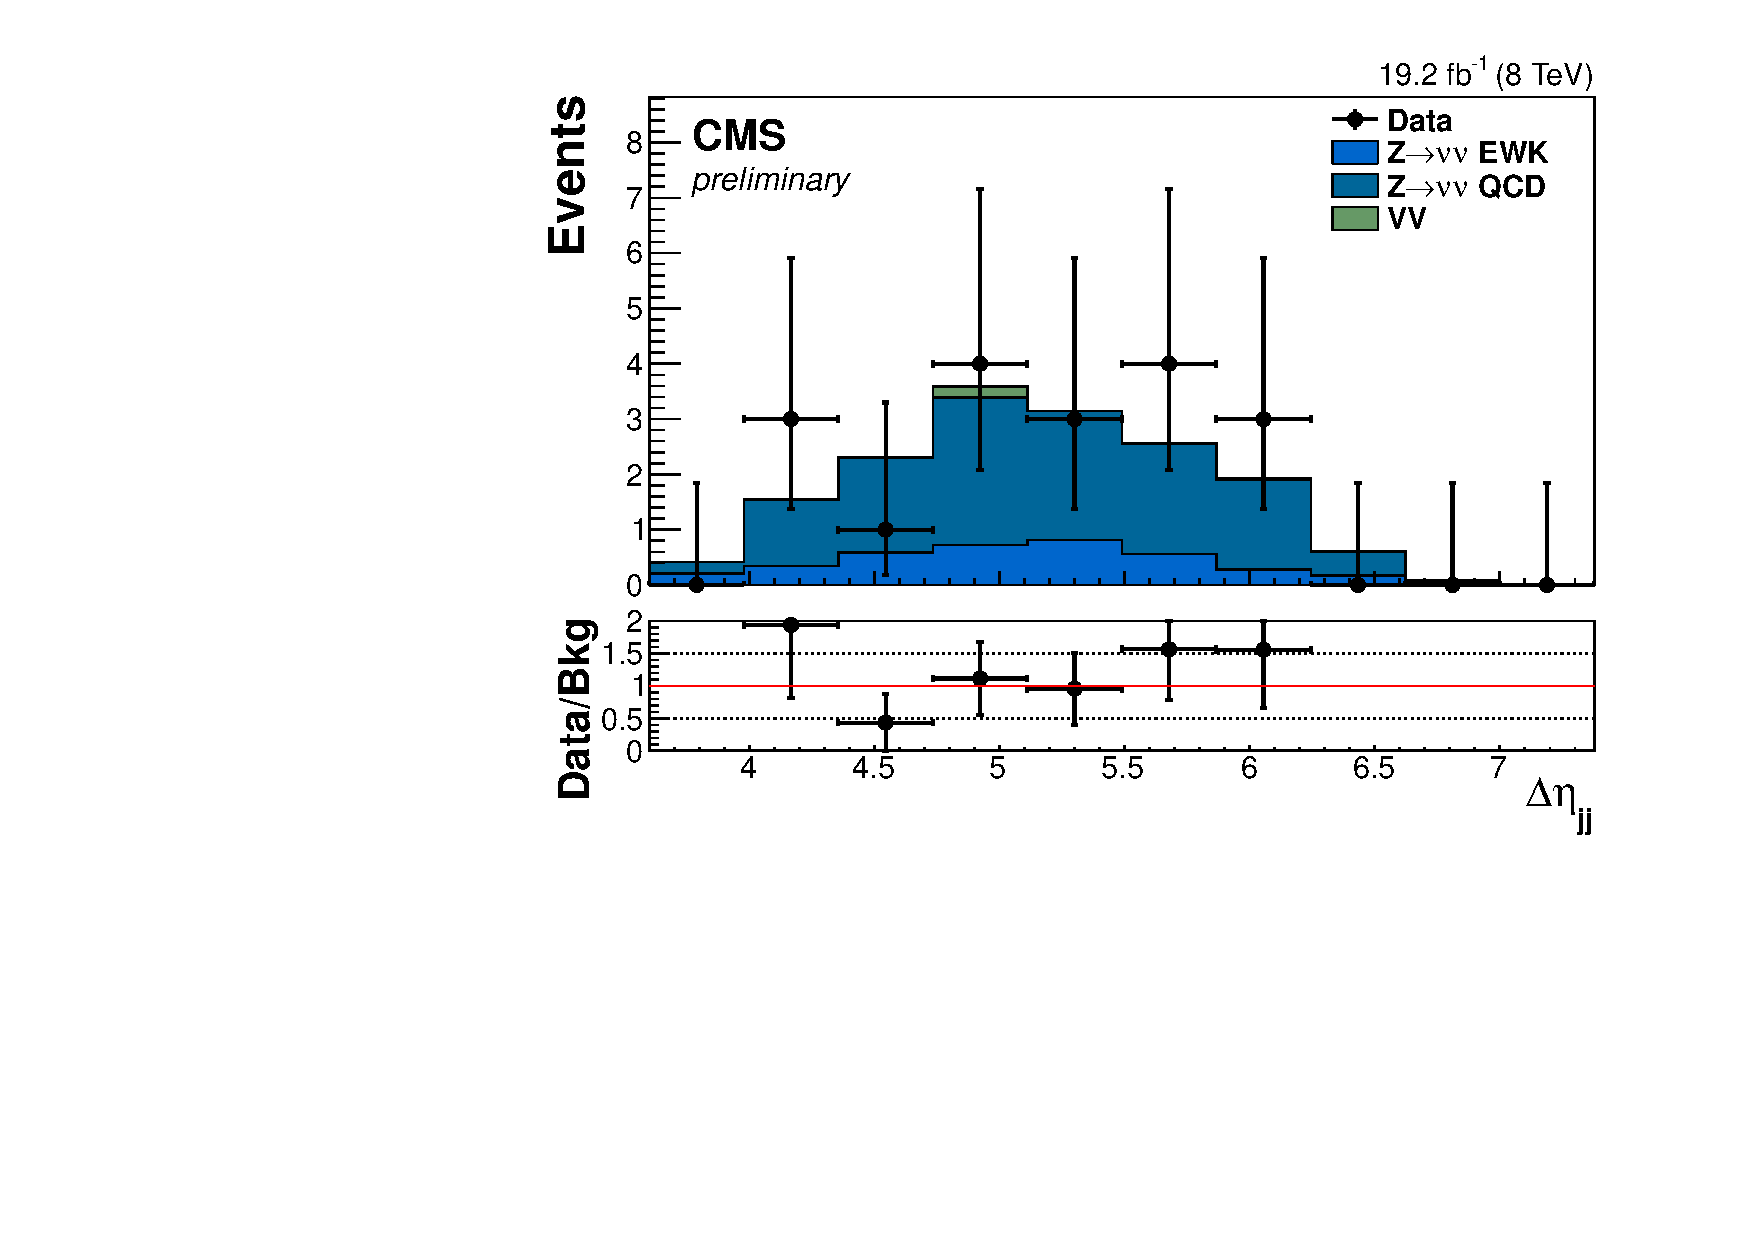
\includegraphics[width=.49\textwidth]{Chapter07/Images/output_sigreg/mumu_dijet_deta.pdf}}
% \subfloat[]{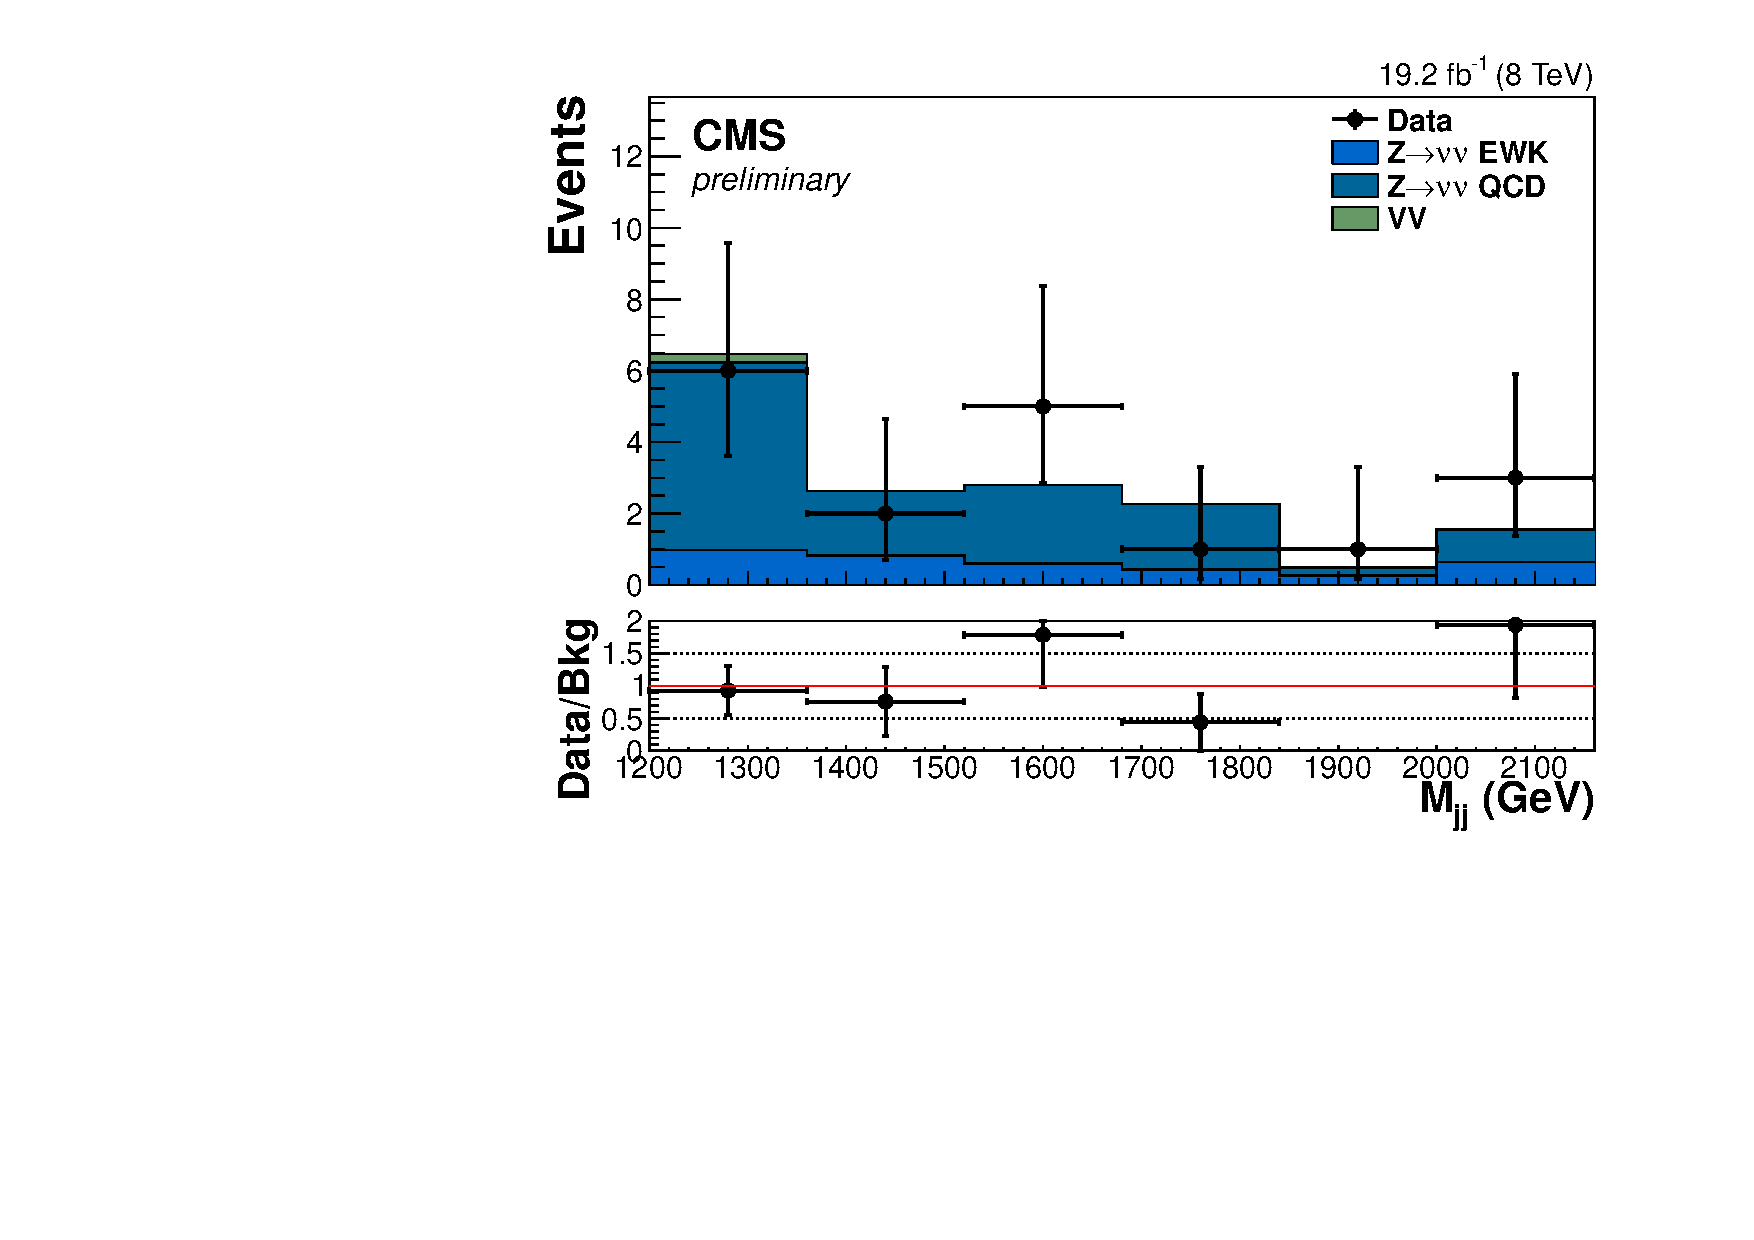
\includegraphics[width=.49\textwidth]{Chapter07/Images/output_sigreg/mumu_dijet_M.pdf}} \\
% \subfloat[]{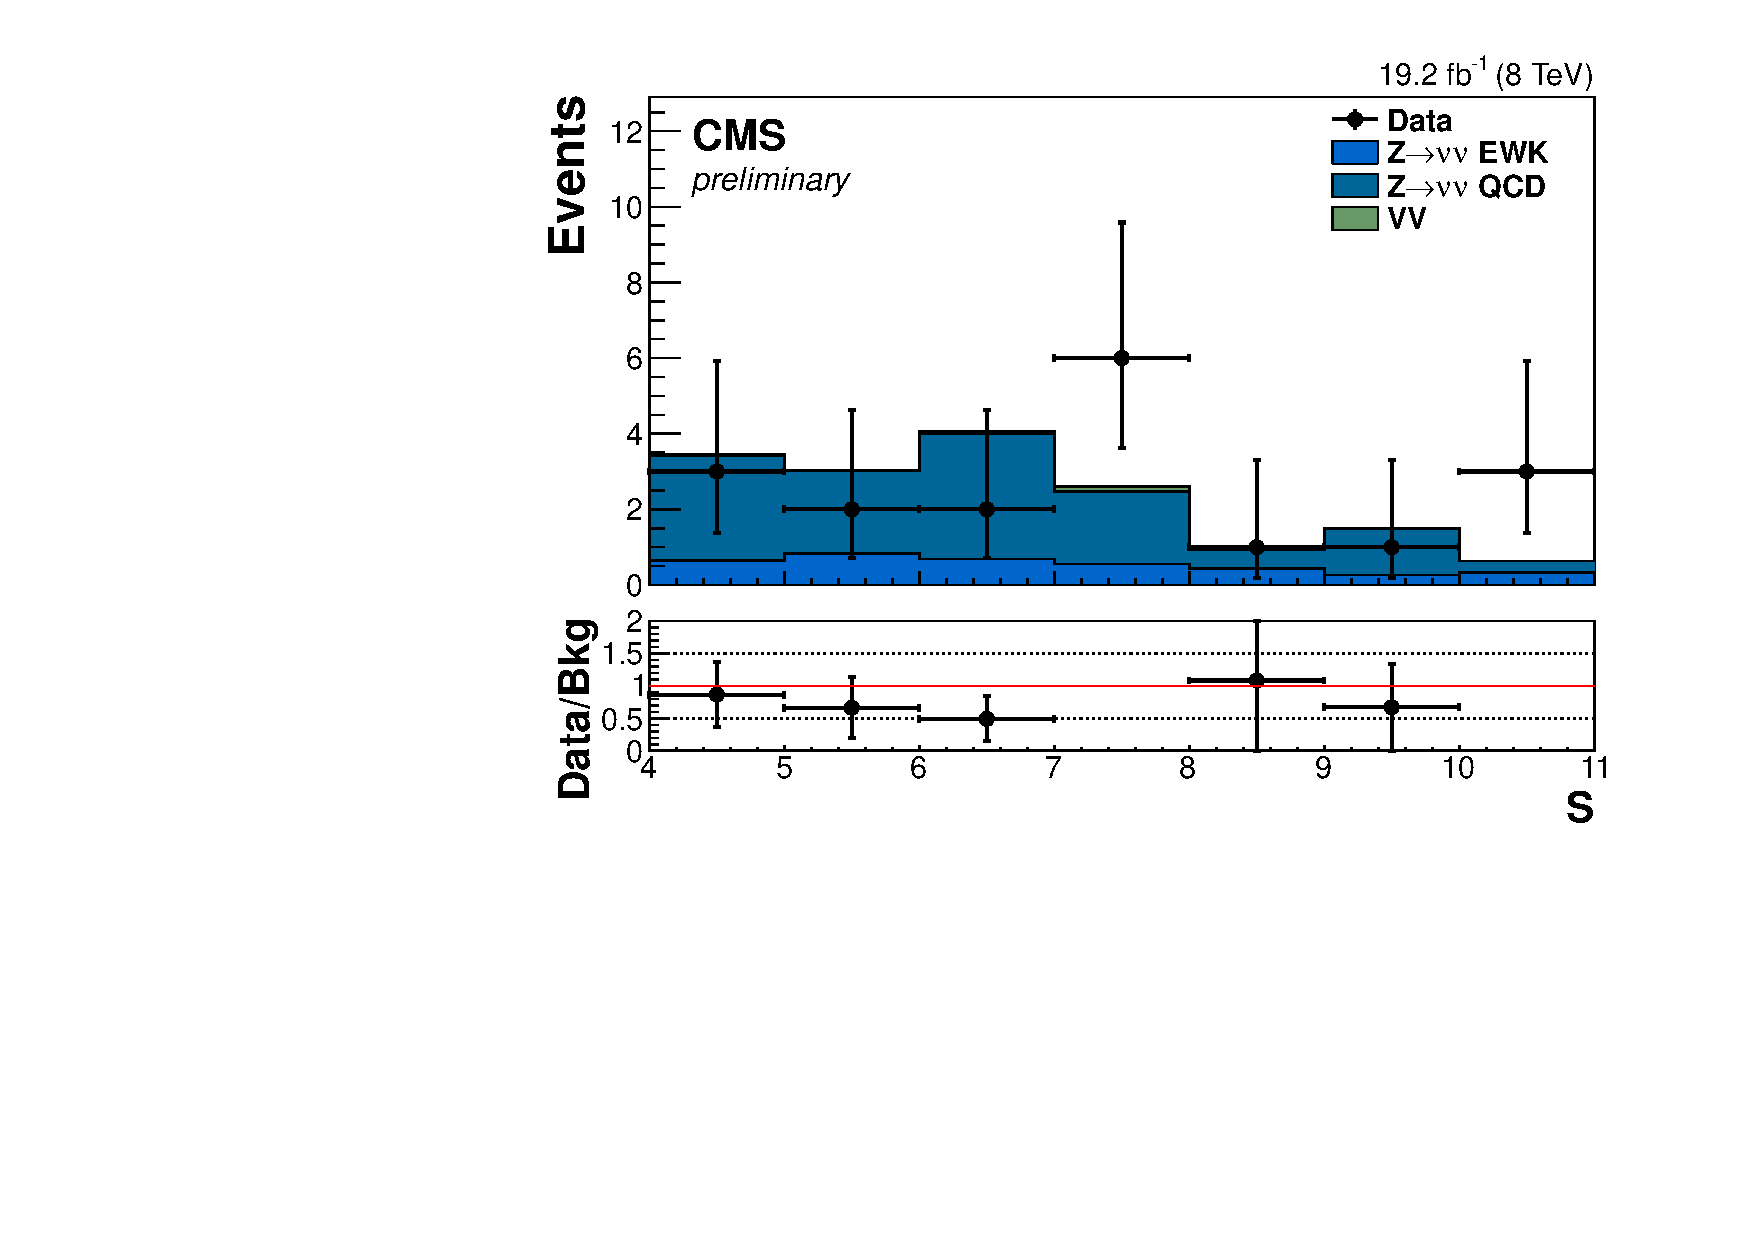
\includegraphics[width=.49\textwidth]{Chapter07/Images/output_sigreg/mumu_metnomu_significance.pdf}}
% \subfloat[]{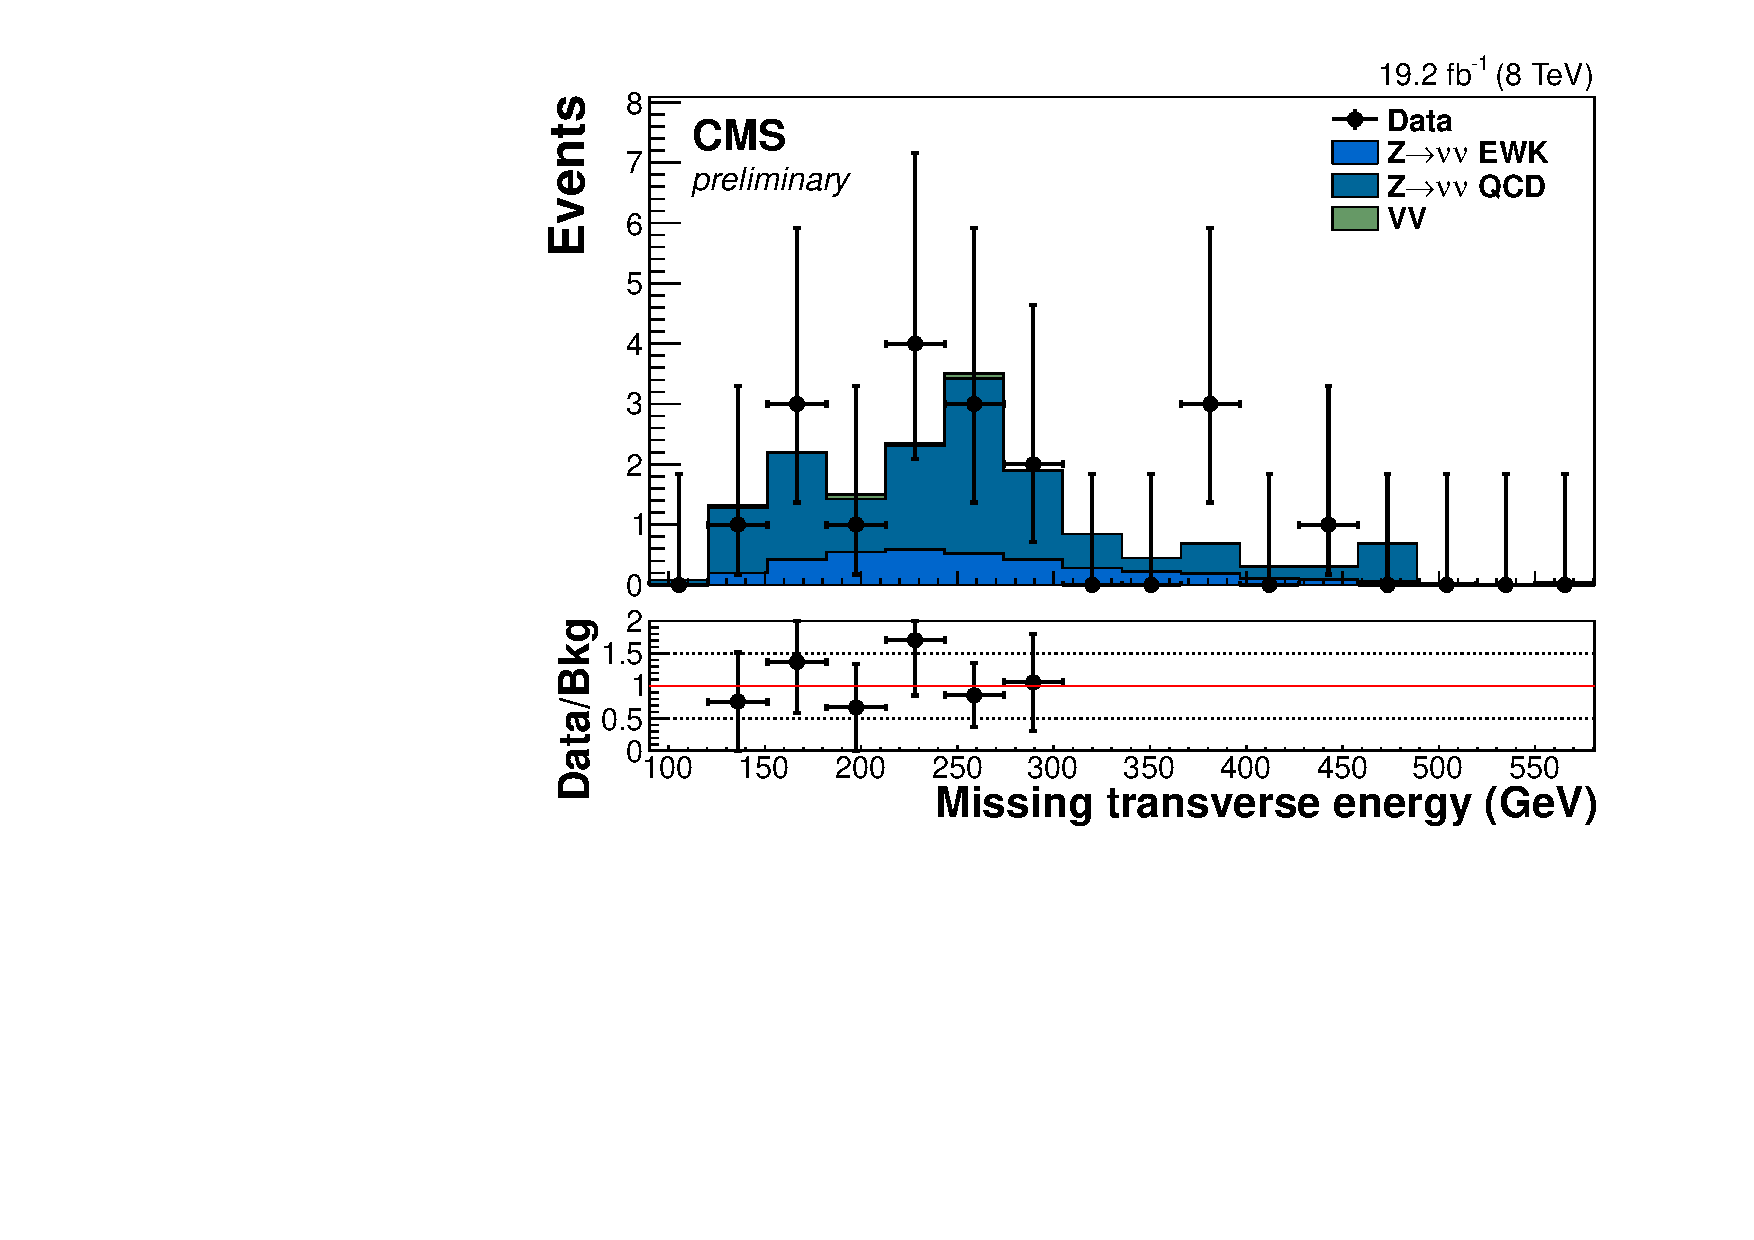
\includegraphics[width=.49\textwidth]{Chapter07/Images/output_sigreg/mumu_metnomuons.pdf}}
% \caption{Distributions of (a) Pseudorapidity difference between the two selected \gls{VBF} jets, $\Delta\eta_{jj}$, (b) Dijet mass $M_{jj}$, (c) \gls{MET} significance $\mathcal{S}$, (d) and \gls{MET}, in the $Z\rightarrow \mu\mu$ control region. The last bin contains the overflow of the distribution \cite{ARTICLE:CMSVBFHiggsInvisibleParkedAnalysisPAS}.}
% \label{FIGURE:ParkedDataAnalysis_ZBackground_KeyDistributions}
% \end{figure}

\begin{figure}[!htb]
\centering
\subfloat[]{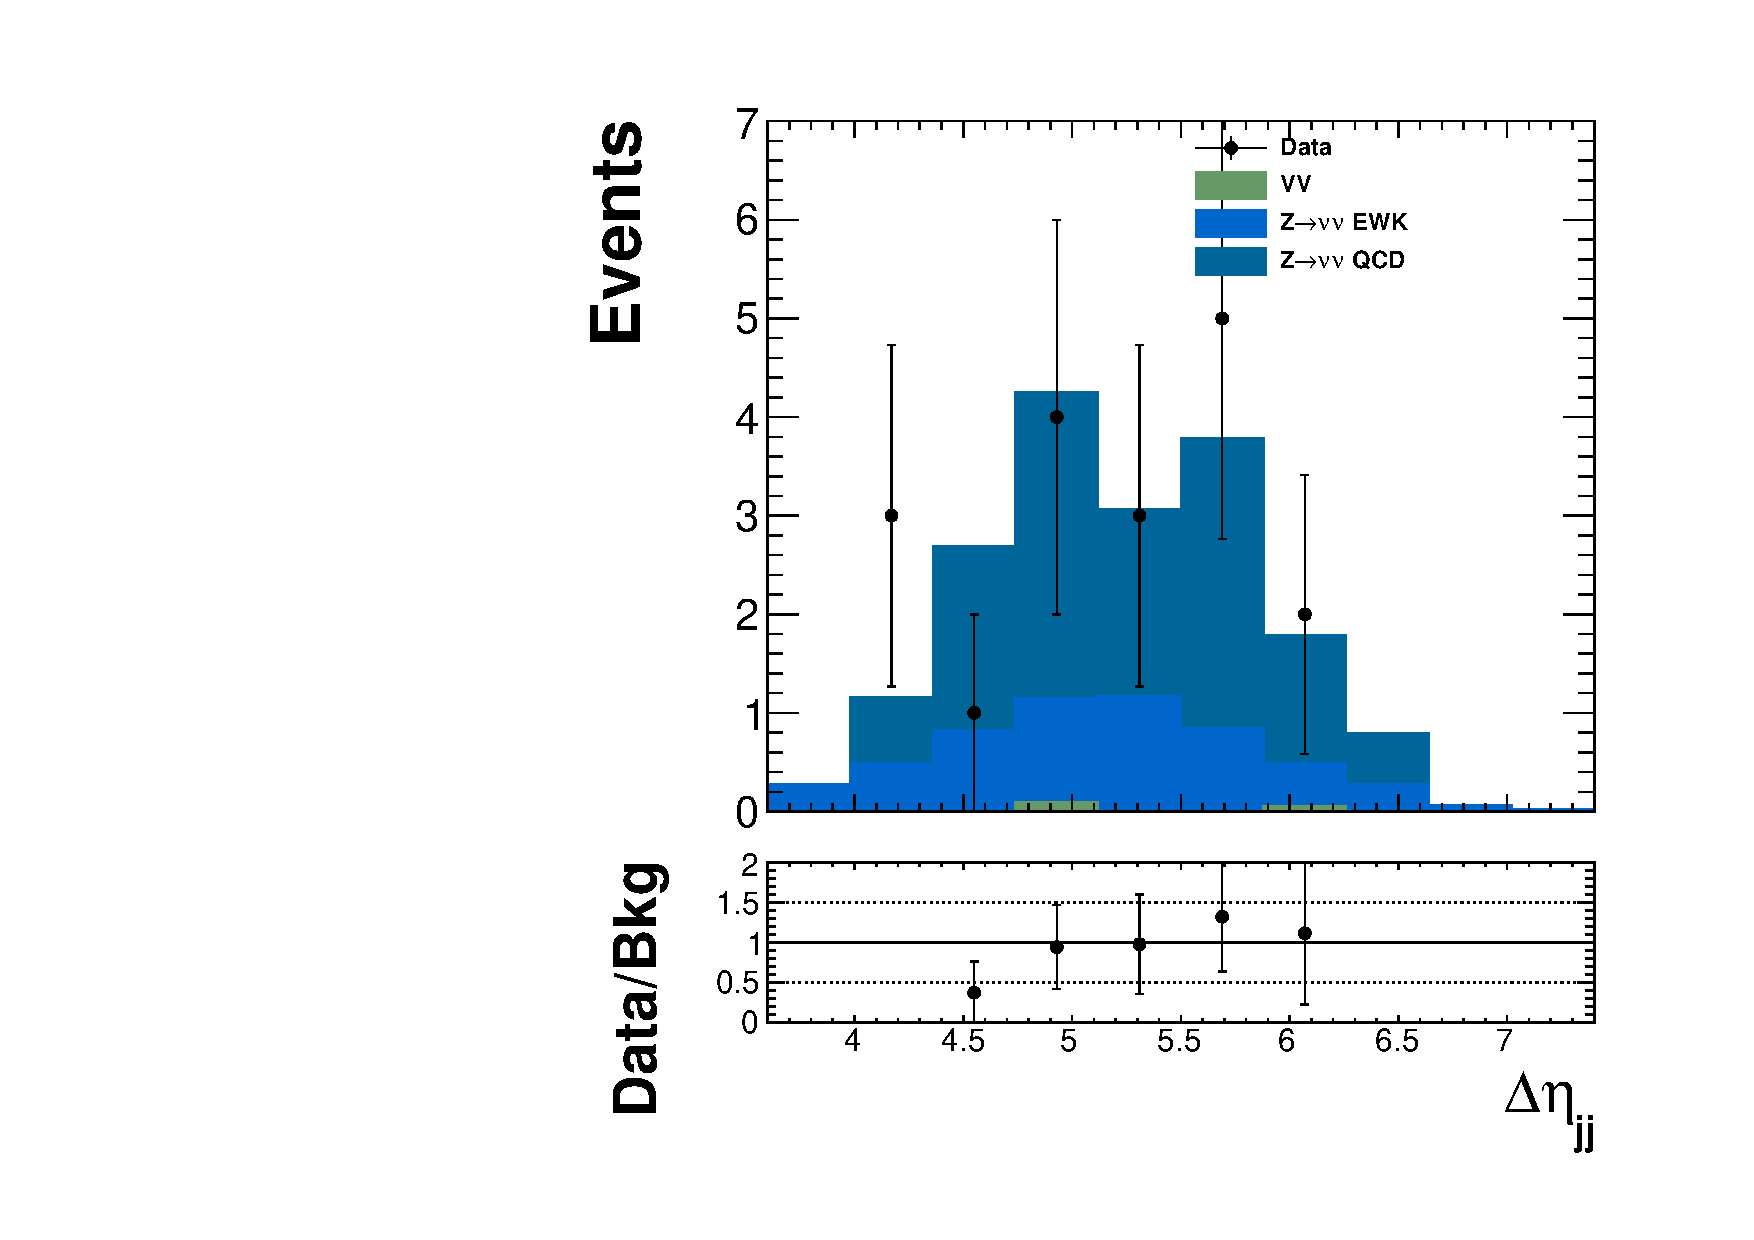
\includegraphics[width=.49\textwidth]{Chapter07/CrossCheck/Zmumu/sigZmumu_Dijet_DeltaEta.pdf}}
\subfloat[]{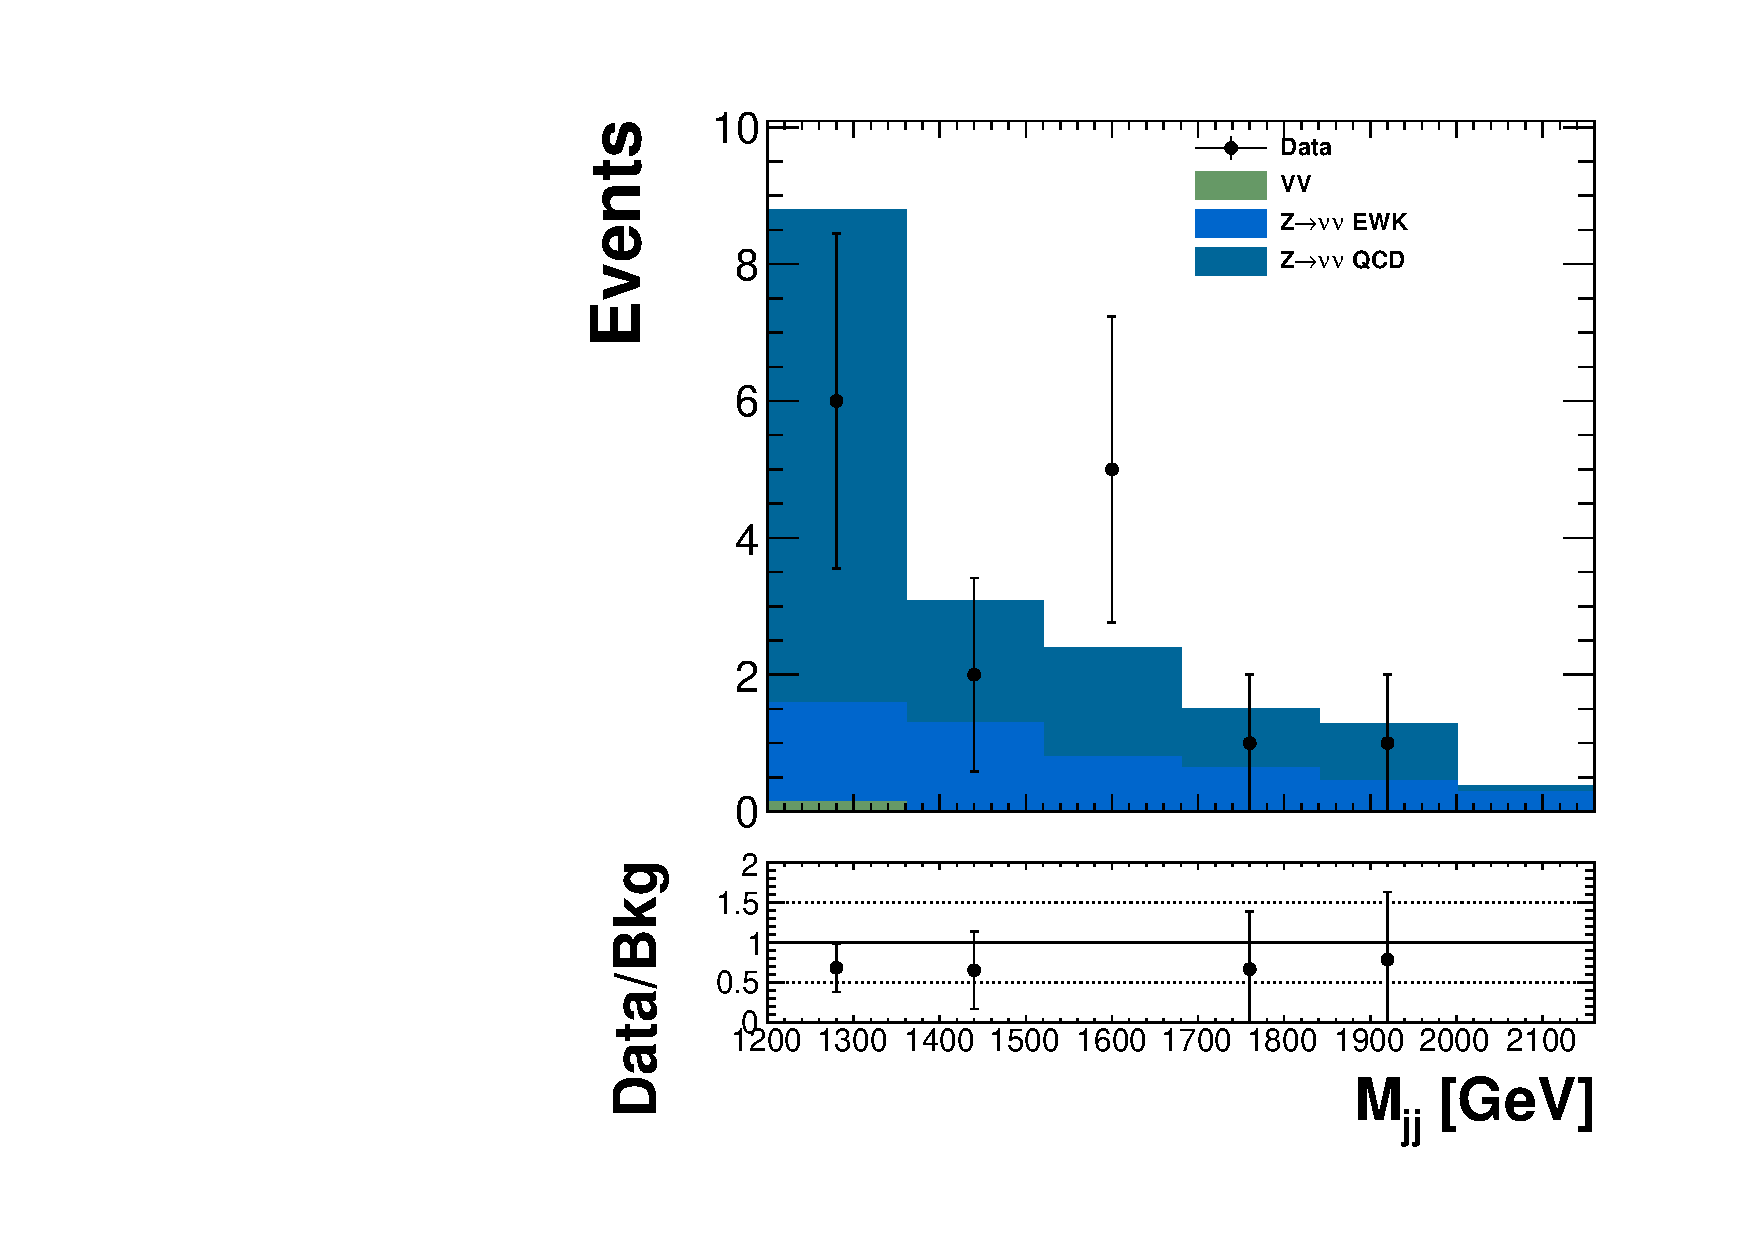
\includegraphics[width=.49\textwidth]{Chapter07/CrossCheck/Zmumu/sigZmumu_Dijet_Mjj.pdf}} \\
\subfloat[]{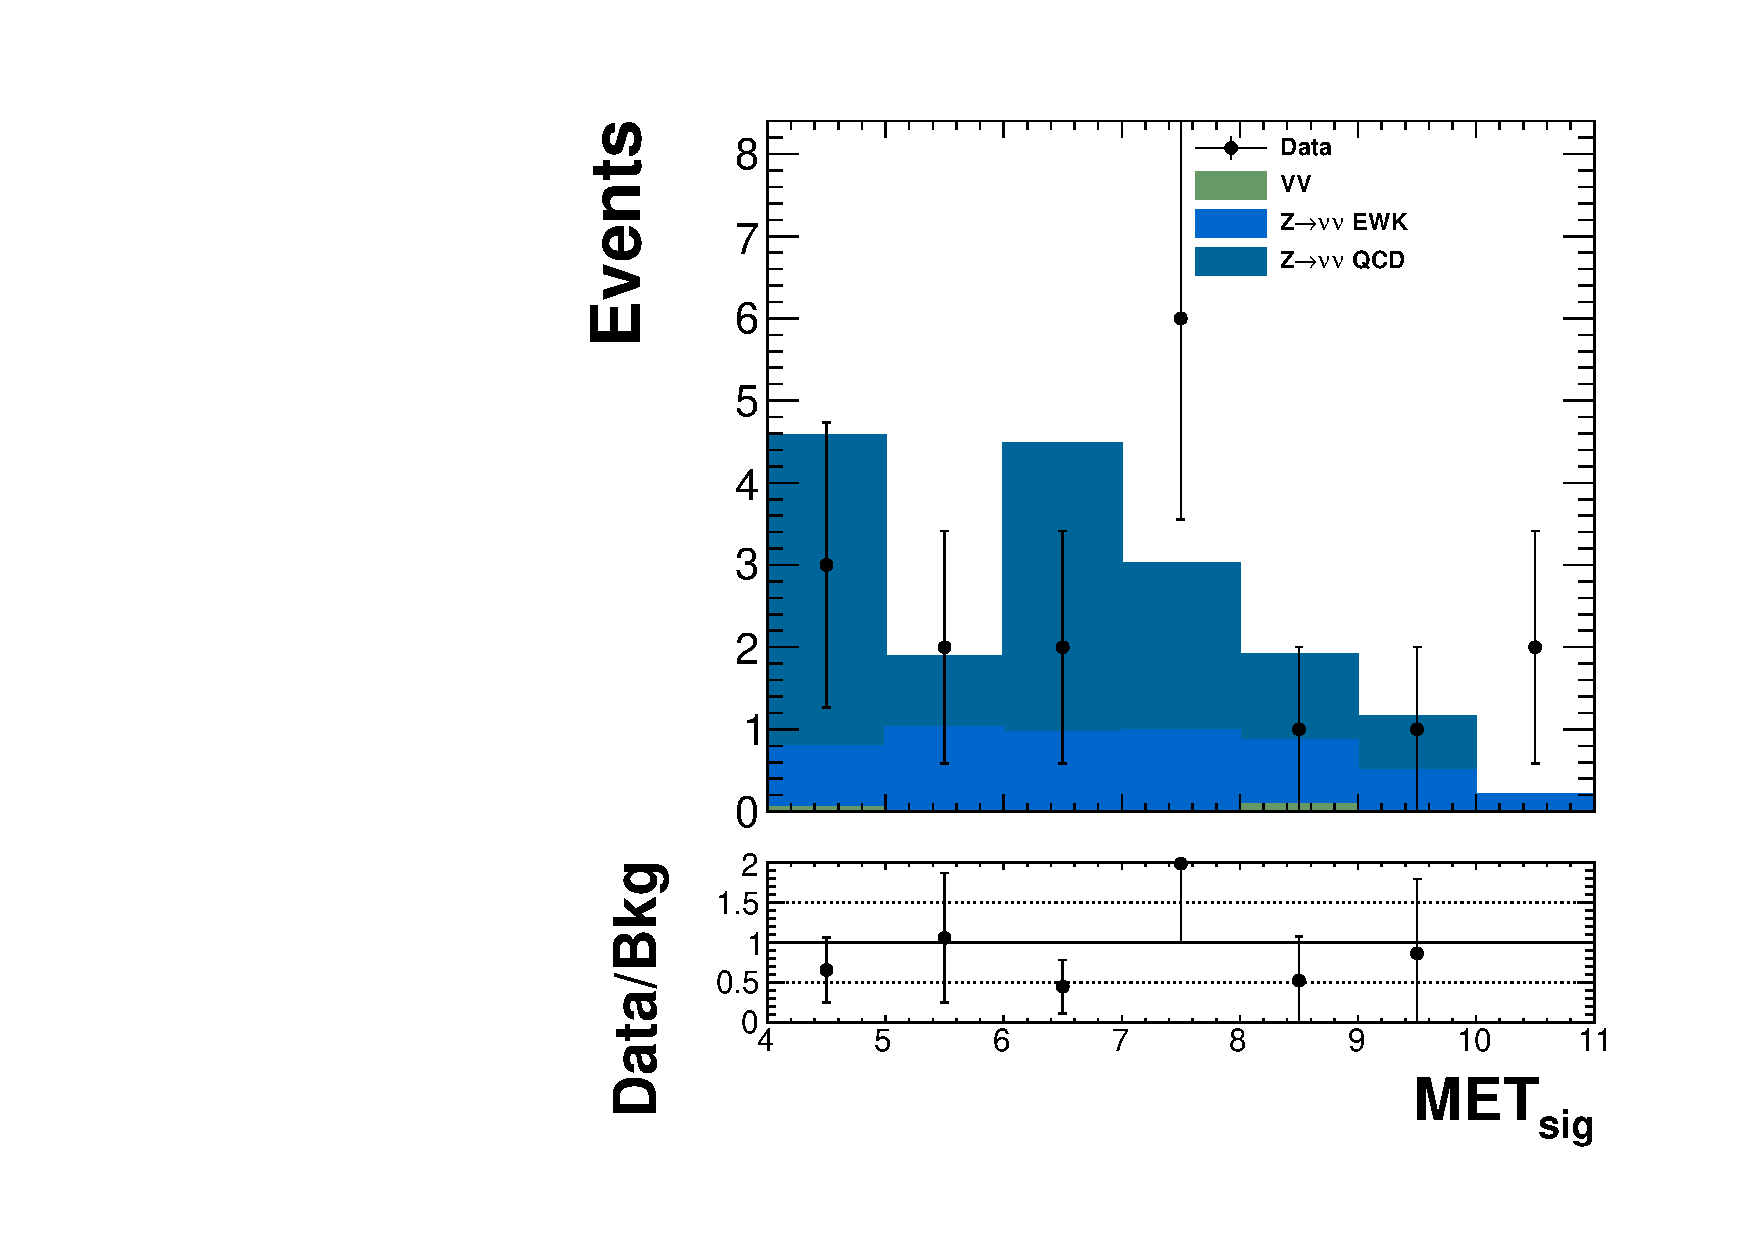
\includegraphics[width=.49\textwidth]{Chapter07/CrossCheck/Zmumu/sigZmumu_metNoMuon_Sig.pdf}}
\subfloat[]{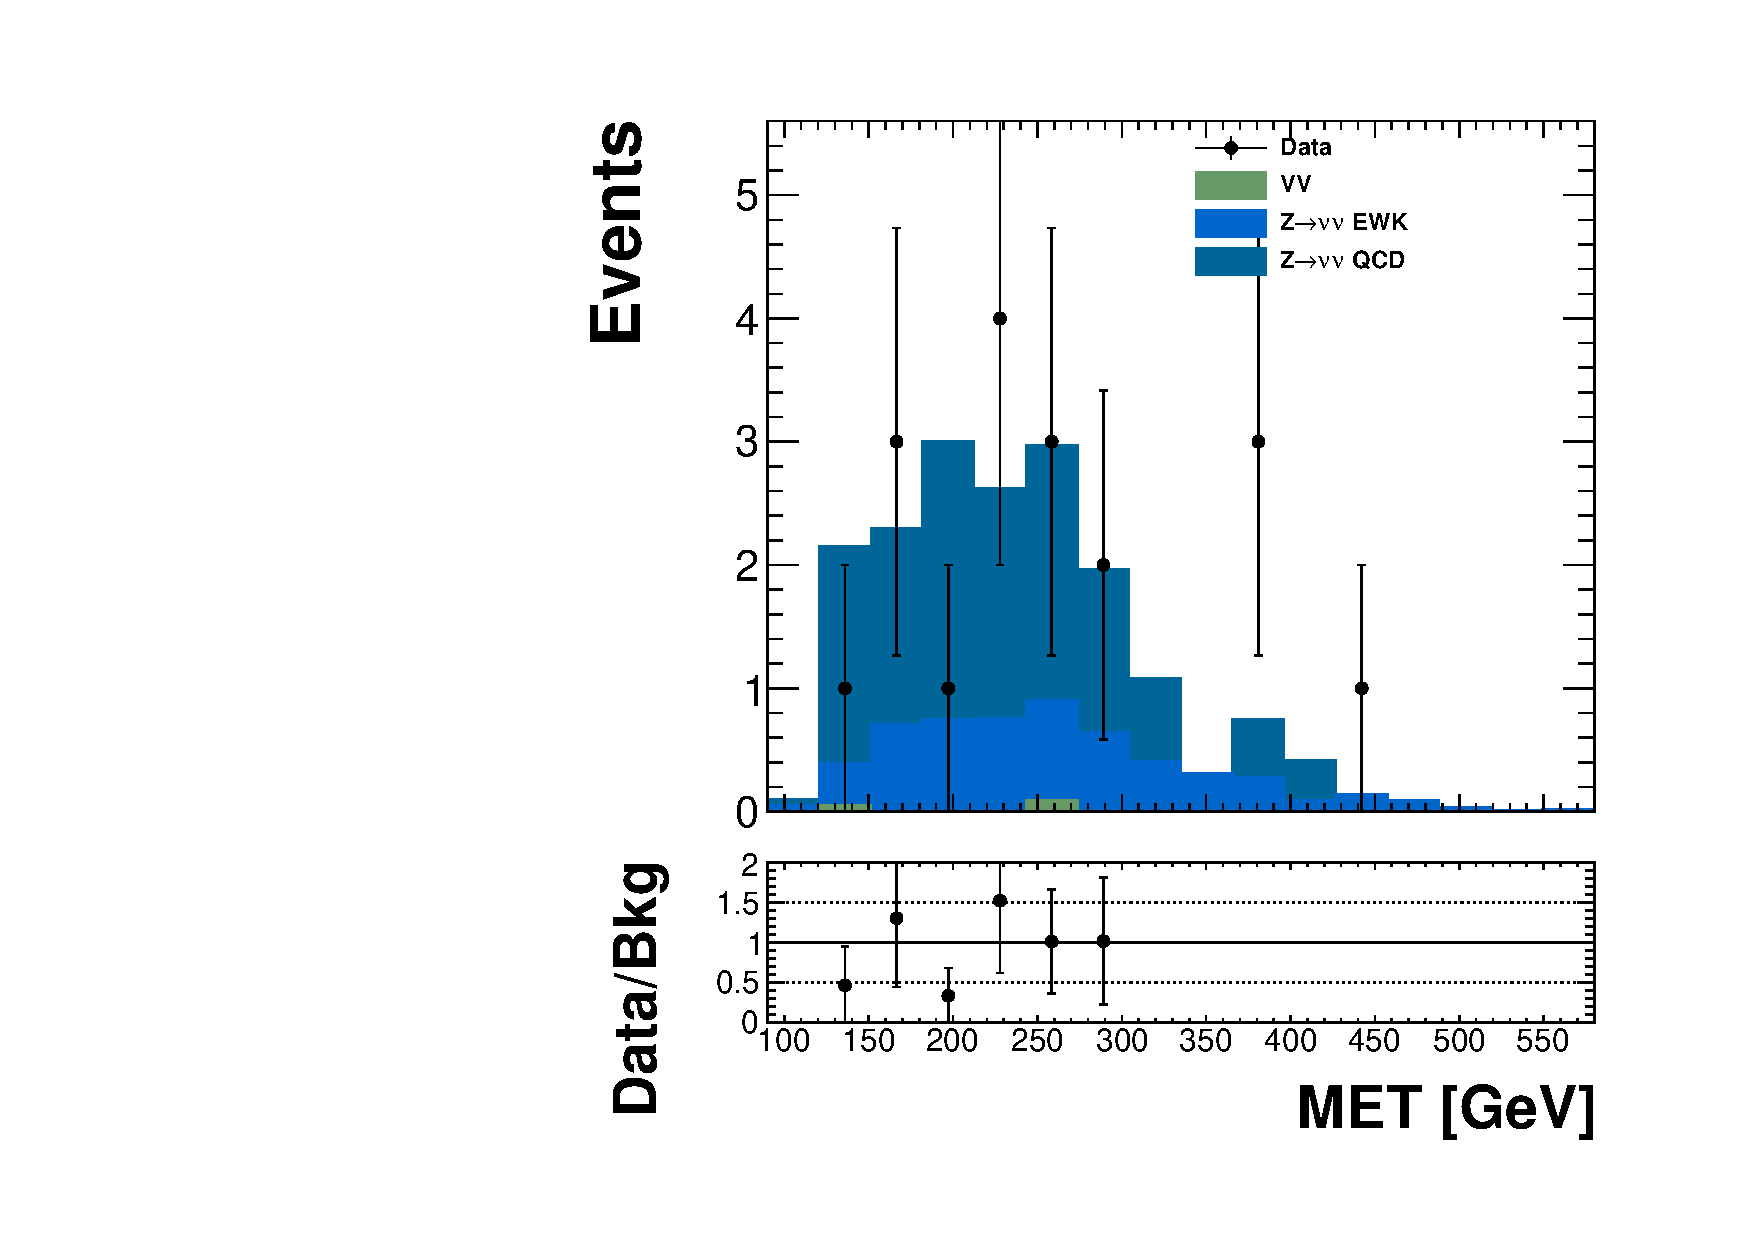
\includegraphics[width=.49\textwidth]{Chapter07/CrossCheck/Zmumu/sigZmumu_metNoMuon.pdf}}
\caption[Distributions of Pseudorapidity difference between the two selected VBF jets, $\Delta\eta_{jj}$, Dijet mass $M_{jj}$, MET significance $\mathcal{S}$ and MET, in the $Z\rightarrow \mu\mu$ control region as seen by the cross check analysis.]
{Distributions of (a) Pseudorapidity difference between the two selected \gls{VBF} jets, $\Delta\eta_{jj}$, (b) Dijet mass $M_{jj}$, (c) \gls{MET} significance $\mathcal{S}$, (d) and \gls{MET}, in the $Z\rightarrow \mu\mu$ control region as seen by the cross check analysis.}
\label{FIGURE:ParkedDataAnalysis_ZBackground_KeyDistributions}
\end{figure}

Good agreement between data and \gls{MC} simulation is observed considering the available statistics. The final estimation of the contribution of the $Z\rightarrow \nu\nu$ background to the signal region is $N_{S}^{Z\rightarrow\nu\nu}= 158.1 \pm 37.8 \stat \pm 21.2 \syst$ for the main analysis and $151.4 \pm 39.0 \stat$ for the cross check analysis. 

%%%%%%%%%%%%%%%%%%%%%%%%%%%%%%%%%%%%%%%%%%%%%%%%%%%%%%%%%%%%%%%%%%%%%%%%%%%%%%%%%%%%
%%% SUBSECTION
%%%%%%%%%%%%%%%%%%%%%%%%%%%%%%%%%%%%%%%%%%%%%%%%%%%%%%%%%%%%%%%%%%%%%%%%%%%%%%%%%%%%
\subsection{W background estimation}
\label{SECTION:ParkedDataAnalysis_ControlRegions_WBackground}

%Status: DONE (reviewed J.Pela x1)

A similar approach is taken for the W background. The control region is defined by the signal region criteria except that we explicitly require the presence of exactly one single lepton (tight electron or tight muon) or hadronic tau. The data event yield obtained in this region is extrapolated to the signal region with a conversion factor determined from \gls{MC} simulation. Equation \ref{EQUATION:ParkedDataAnalysis_WBackground} is used to obtain the predicted number of events in the signal region.

\begin{align}
%   \begin{split}
%   \end{split}
N_{S}^{W}&=N_{S}^{W\,MC}\frac{N_{C}^{Data}-N_{C}^{bkg}}{N_{C}^{W\,MC}}=N_{S}^{W\,MC}\cdot \rm{SF}
\label{EQUATION:ParkedDataAnalysis_WBackground}
\end{align}

The prediction of each W decay channel is calculated separately for e, $\mu$ (which include $W\rightarrow\tau\nu\rightarrow \nu_\tau l\nu_l$ with $l$ equal to e and $\mu$ respectively) and hadronic $\tau$. In these control regions the number of events from other backgrounds $N_{C}^{bkg}$ is mainly composed of events from top processes which are estimated from \gls{MC}.

In the W$\rightarrow\tau_{\mathrm{h}}\nu$ control region, a very small number of events pass the $\Delta\phi(\text{MET},jets)$ requirement. In order to increase the event statistics, this is replaced by a requirement that the minimal azimuthal angle separation between the \gls{MET} and one of the leading two jets $\Delta\phi(\text{MET},jet_{1,2})$ is greater than 1. To reject events from \gls{QCD} multi-jet processes, an additional requirement on the transverse mass of the W to be greater than $20\,\GeV$ is used. The W$\rightarrow\mu\nu$ region has enough statistics to study the full range of $\Delta\phi(\text{MET},jets)$ A 20\% systematic uncertainty is added to account for the observed difference in shape of the $\Delta\phi(\text{MET},jets)$ variable observed between \gls{MC} simulation and data. Distributions of $M_{jj}$, \gls{MET} and $\Delta\phi(\text{MET},jets)$ are shown in figures \ref{FIGURE:ParkedDataAnalysis_WBackground_Mjj}, \ref{FIGURE:ParkedDataAnalysis_WBackground_MetNoMu} and \ref{FIGURE:ParkedDataAnalysis_WBackground_MinDeltaPhi}

\begin{figure}[!htb]
\centering
\subfloat[]{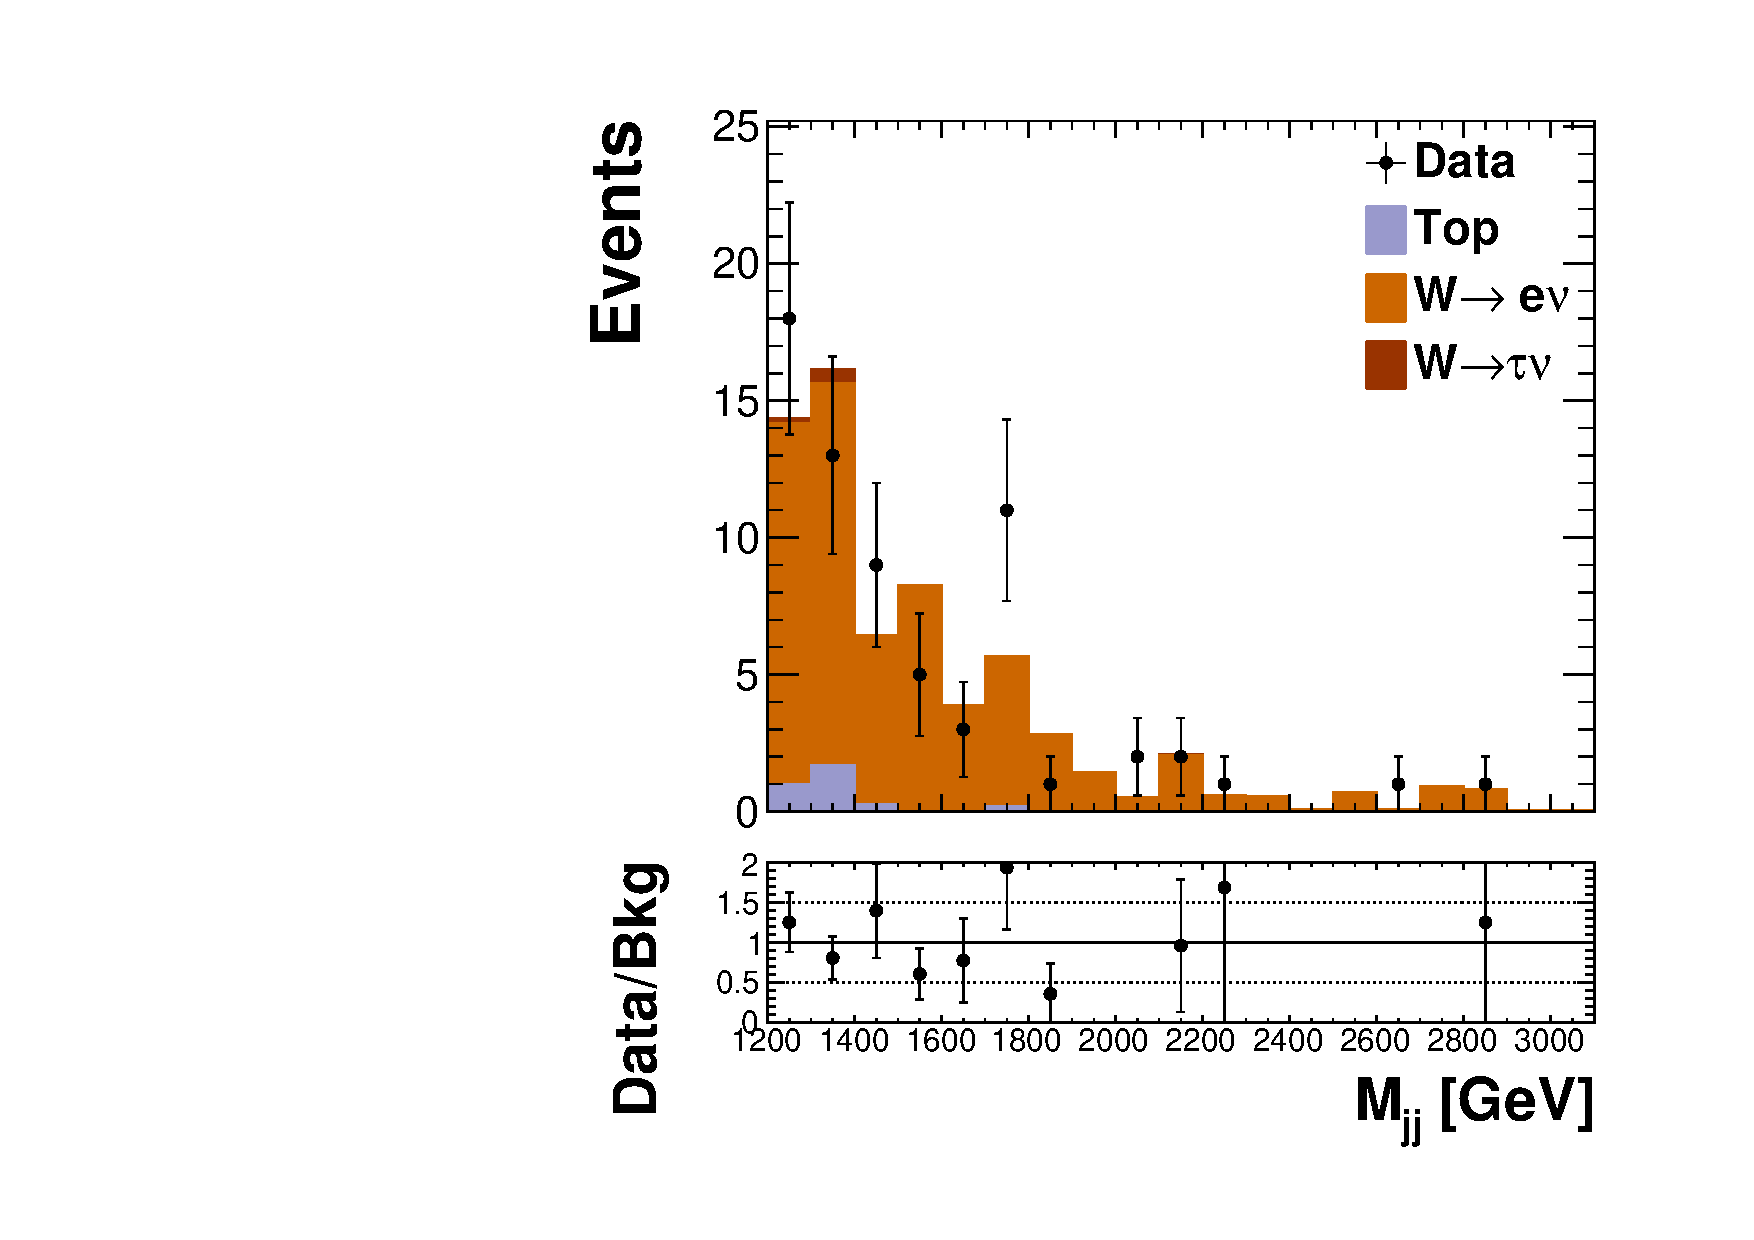
\includegraphics[width=.45\textwidth]{Chapter07/CrossCheck/Wenu/sigWel_Dijet_Mjj.pdf}}
\subfloat[]{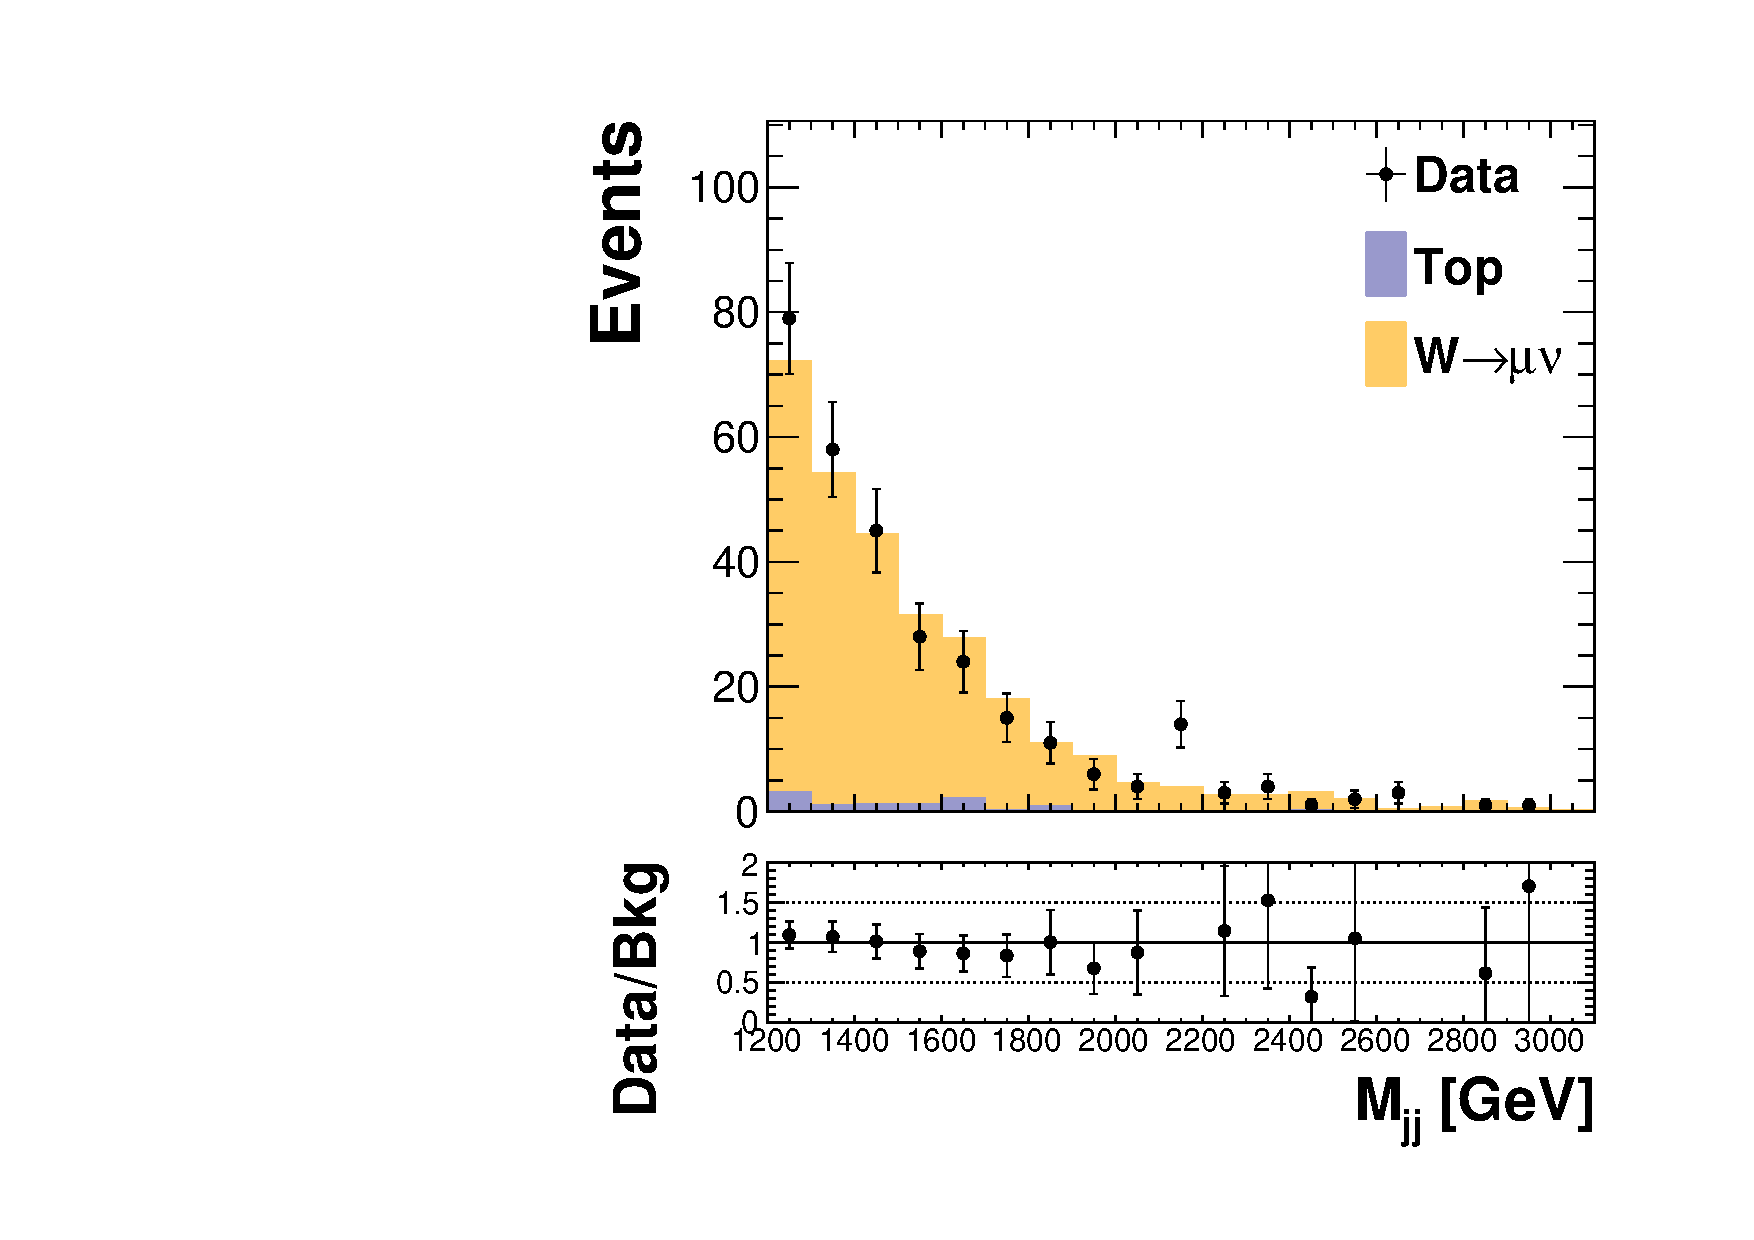
\includegraphics[width=.45\textwidth]{Chapter07/CrossCheck/Wmunu/sigWmu_Dijet_Mjj.pdf}} \\
\subfloat[]{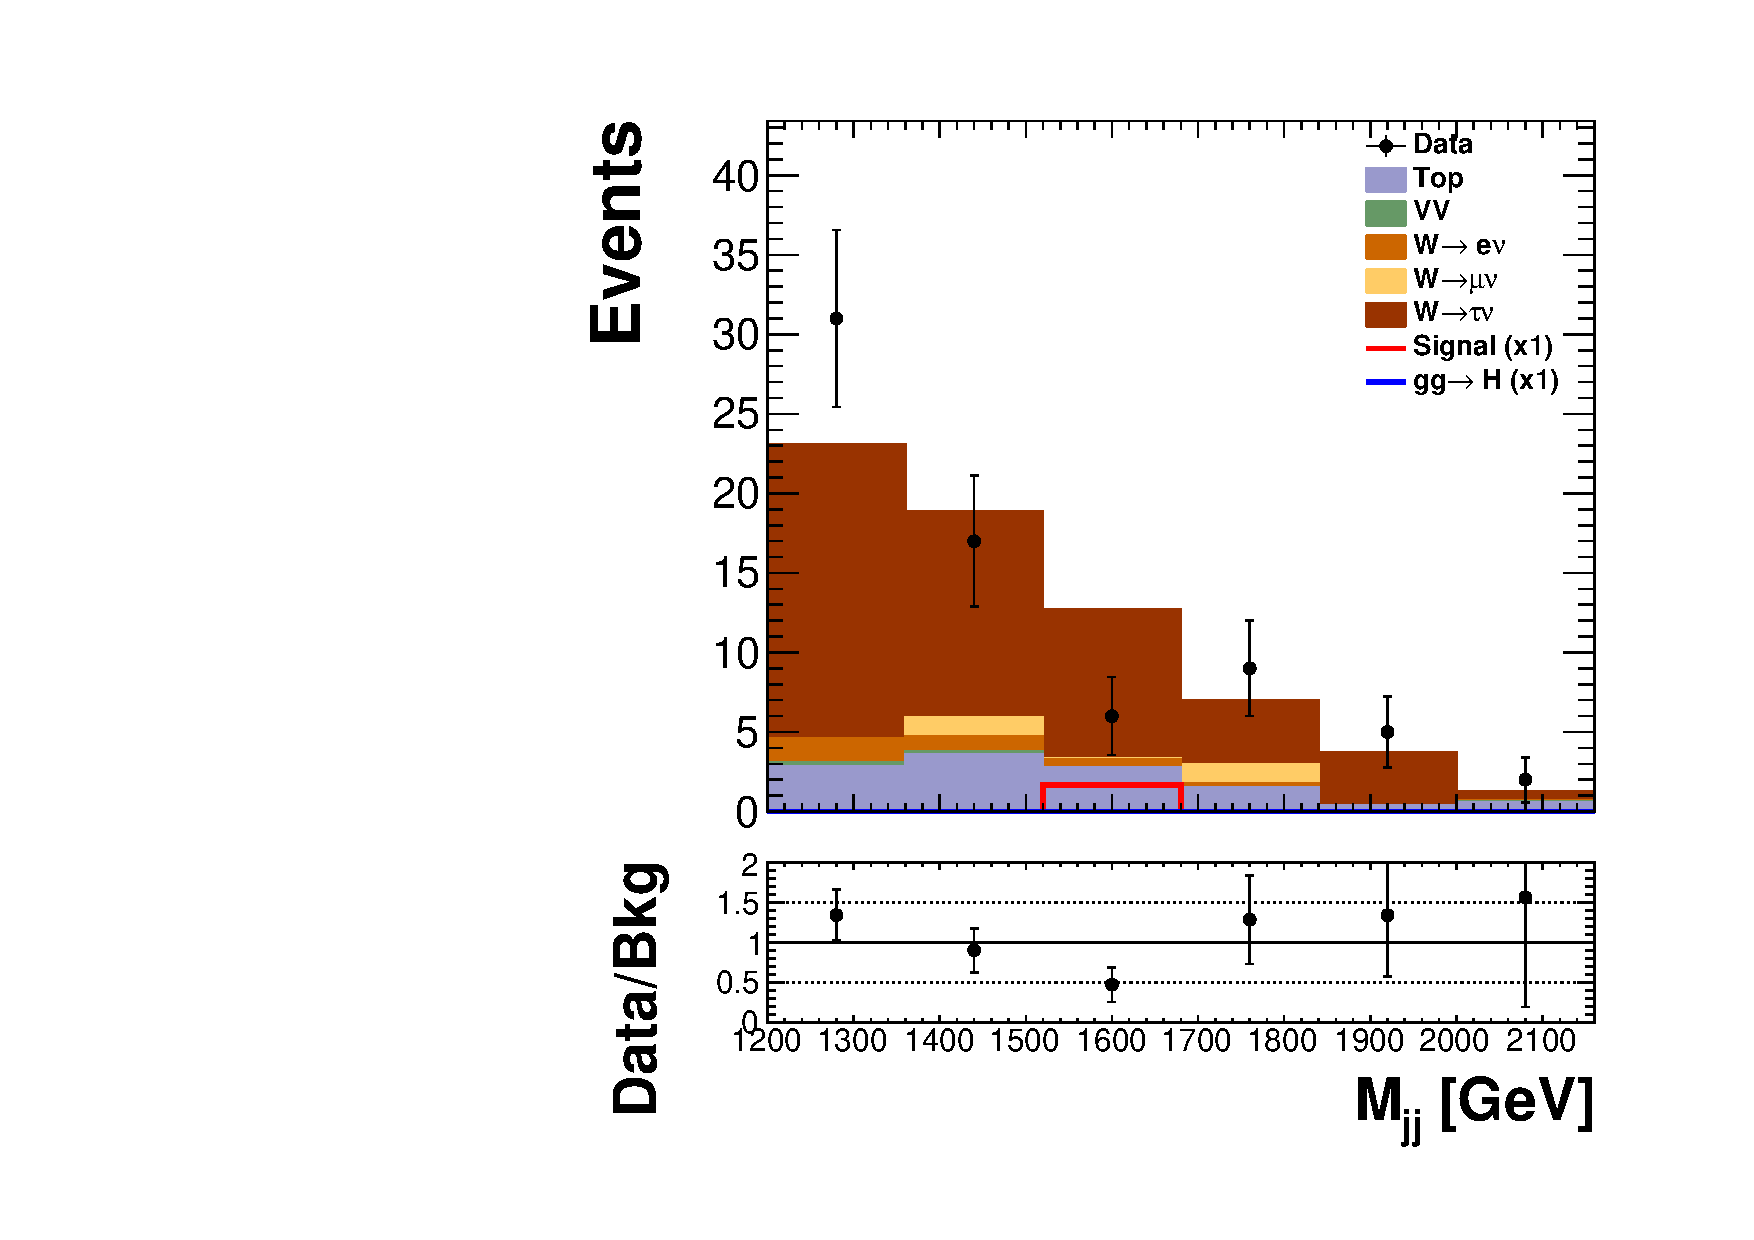
\includegraphics[width=.45\textwidth]{Chapter07/CrossCheck/Wtaunu/sigWta_Dijet_Mjj.pdf}}
\caption[Dijet mass $M_{jj}$ for the $W\rightarrow e\nu$, $W\rightarrow\mu\nu$ and $W\rightarrow\tau\nu$ control regions obtained with the cross check analysis.]
{Dijet mass $M_{jj}$ for the (a) $W\rightarrow e\nu$, (b) $W\rightarrow\mu\nu$ and (c) $W\rightarrow\tau\nu$ control regions obtained with the cross check analysis.}
\label{FIGURE:ParkedDataAnalysis_WBackground_Mjj}
\end{figure}

\begin{figure}[!htb]
\centering
\subfloat[]{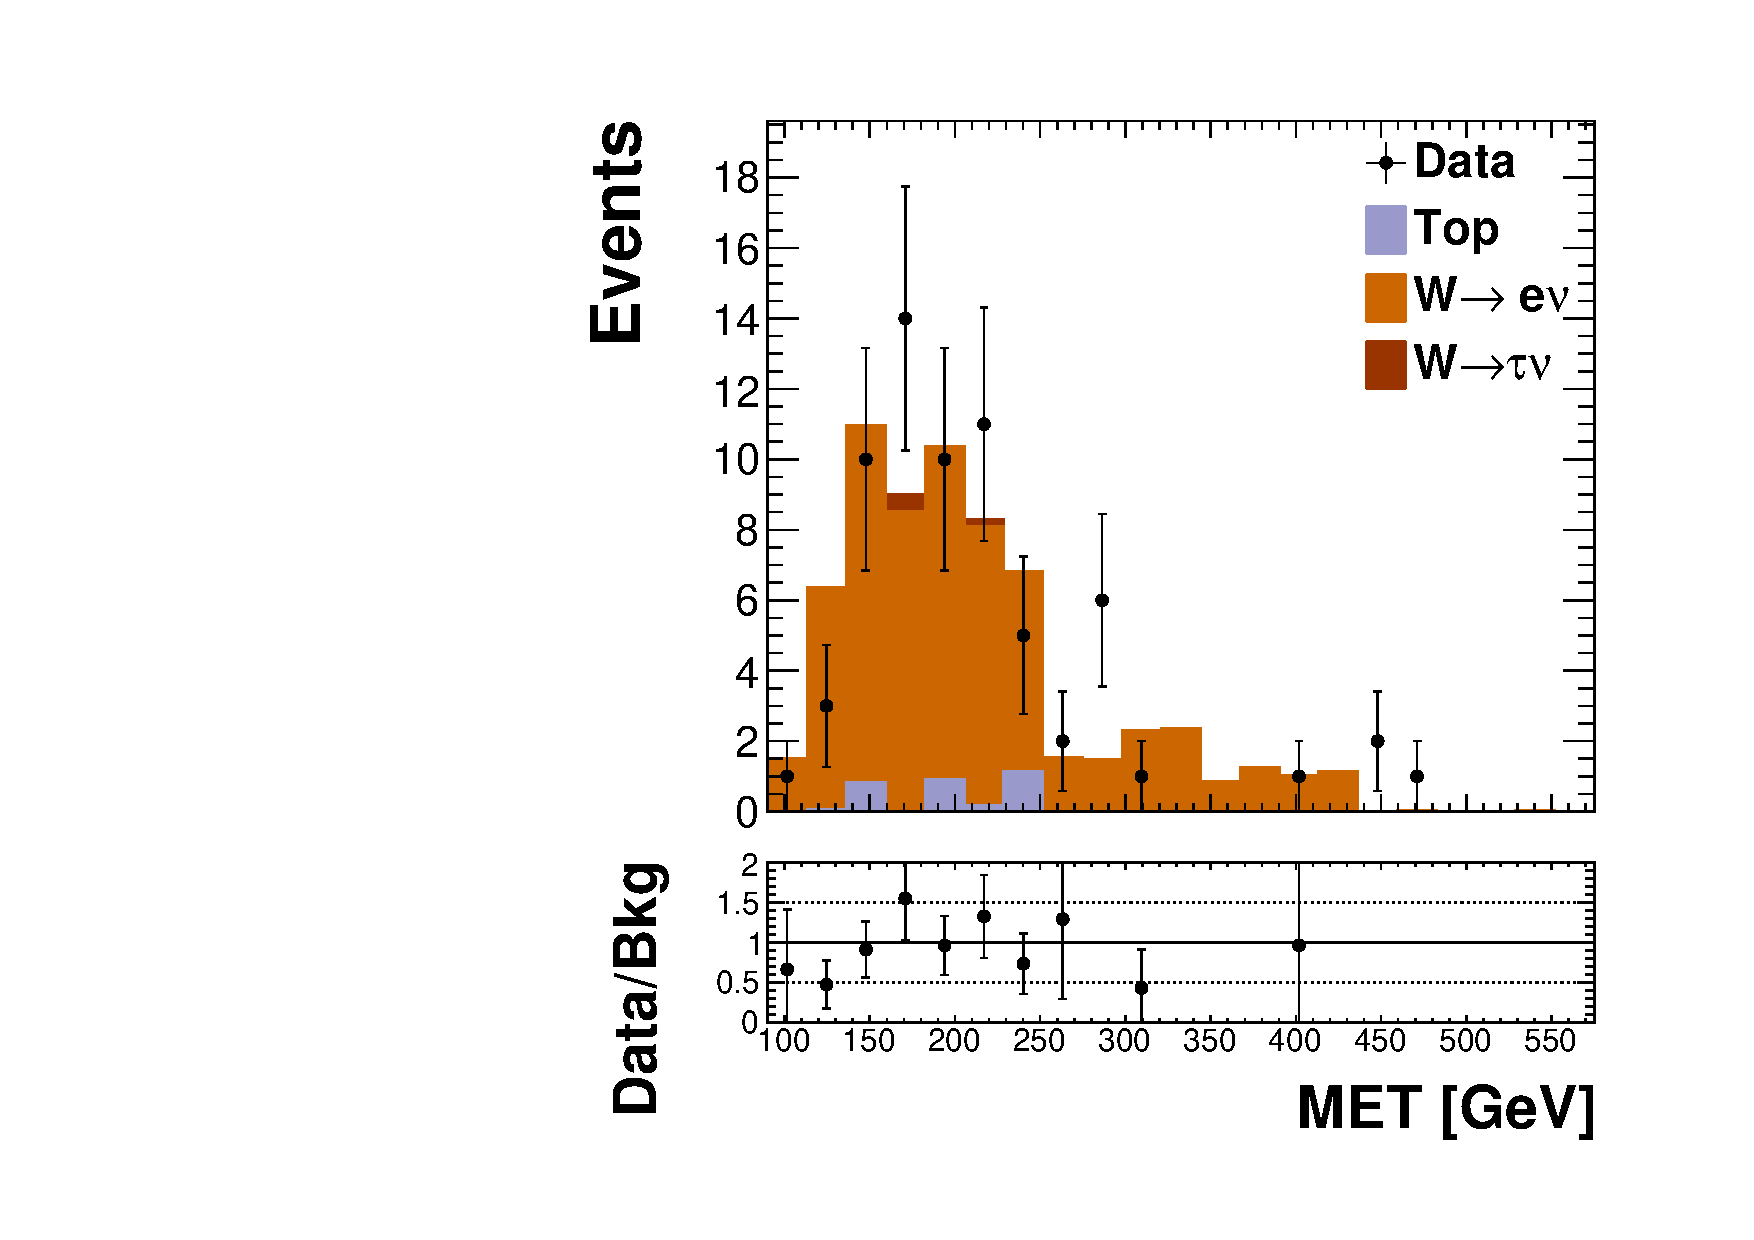
\includegraphics[width=.45\textwidth]{Chapter07/CrossCheck/Wenu/sigWel_metNoMuon.pdf}}
\subfloat[]{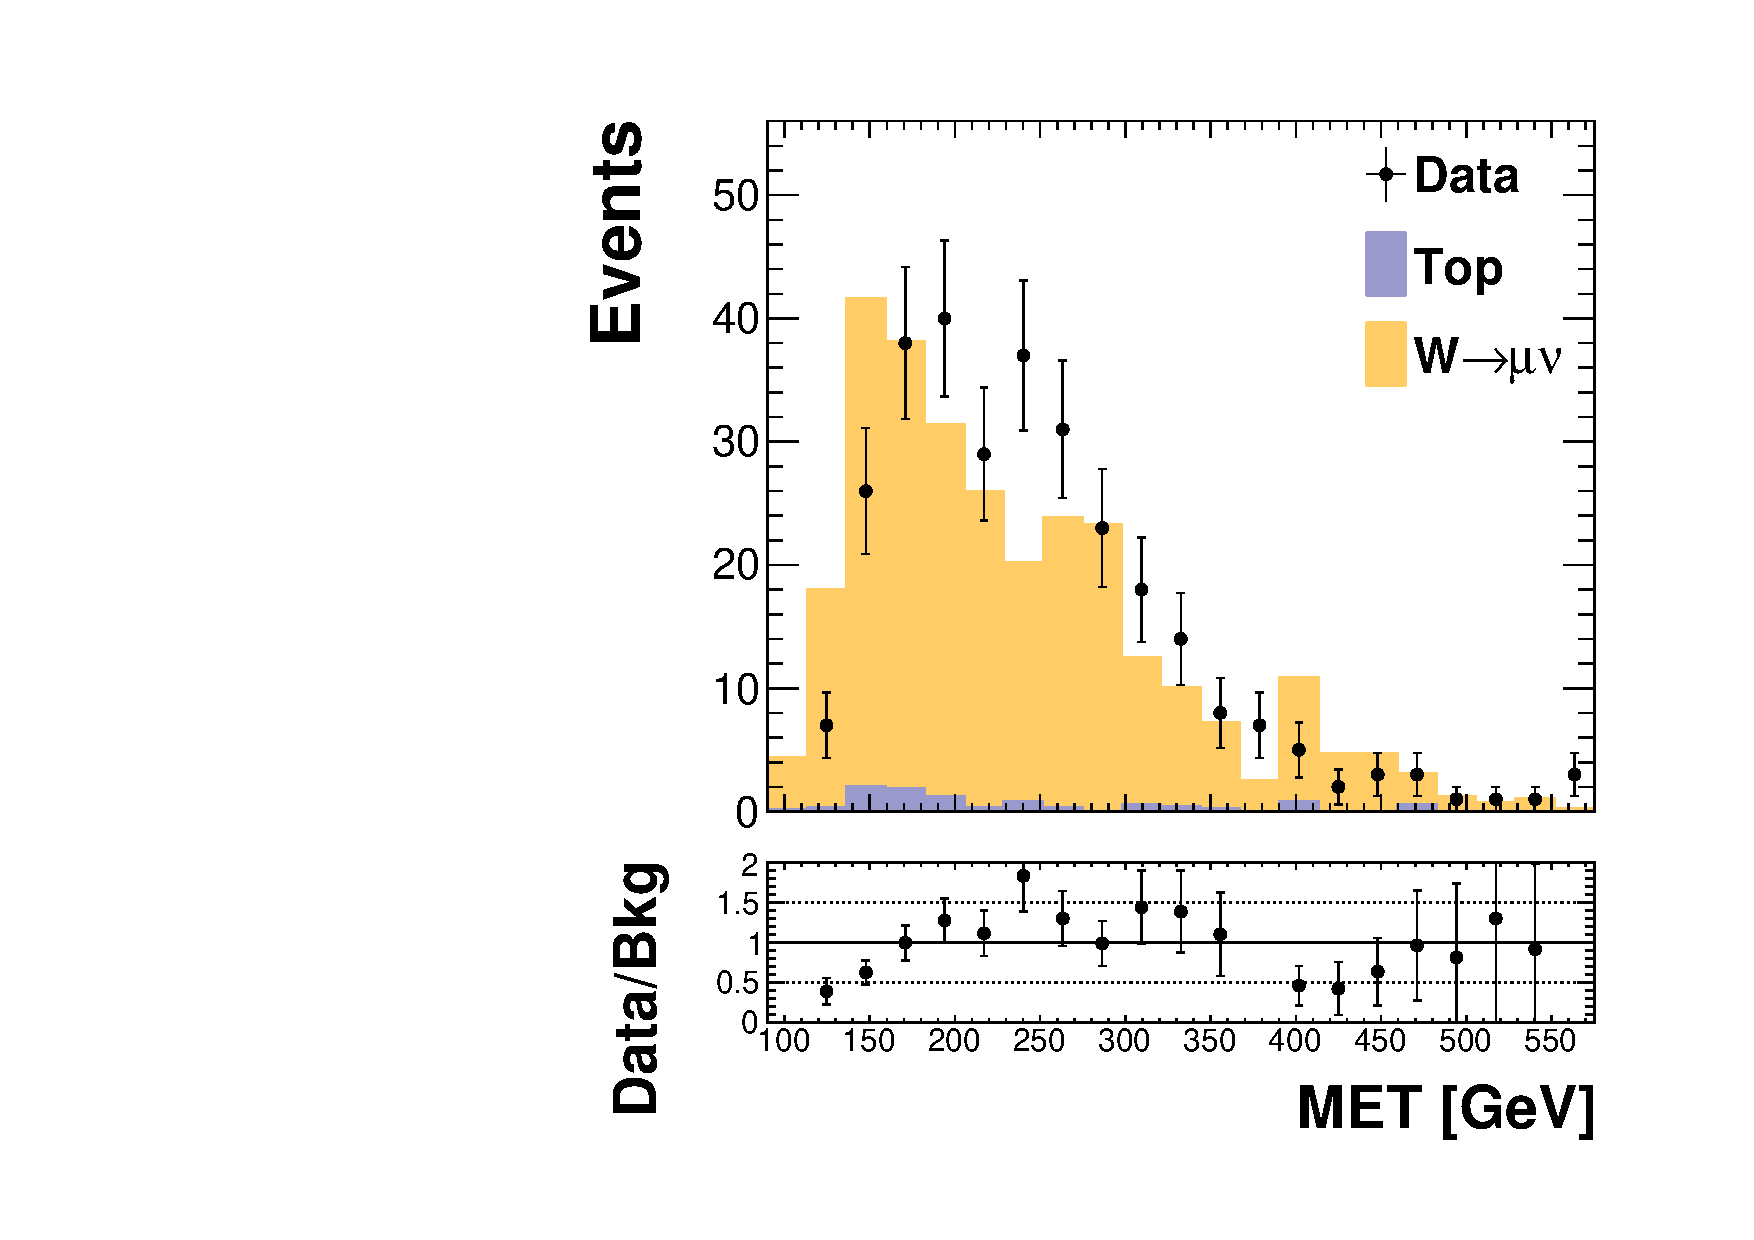
\includegraphics[width=.45\textwidth]{Chapter07/CrossCheck/Wmunu/sigWmu_metNoMuon.pdf}} \\
\subfloat[]{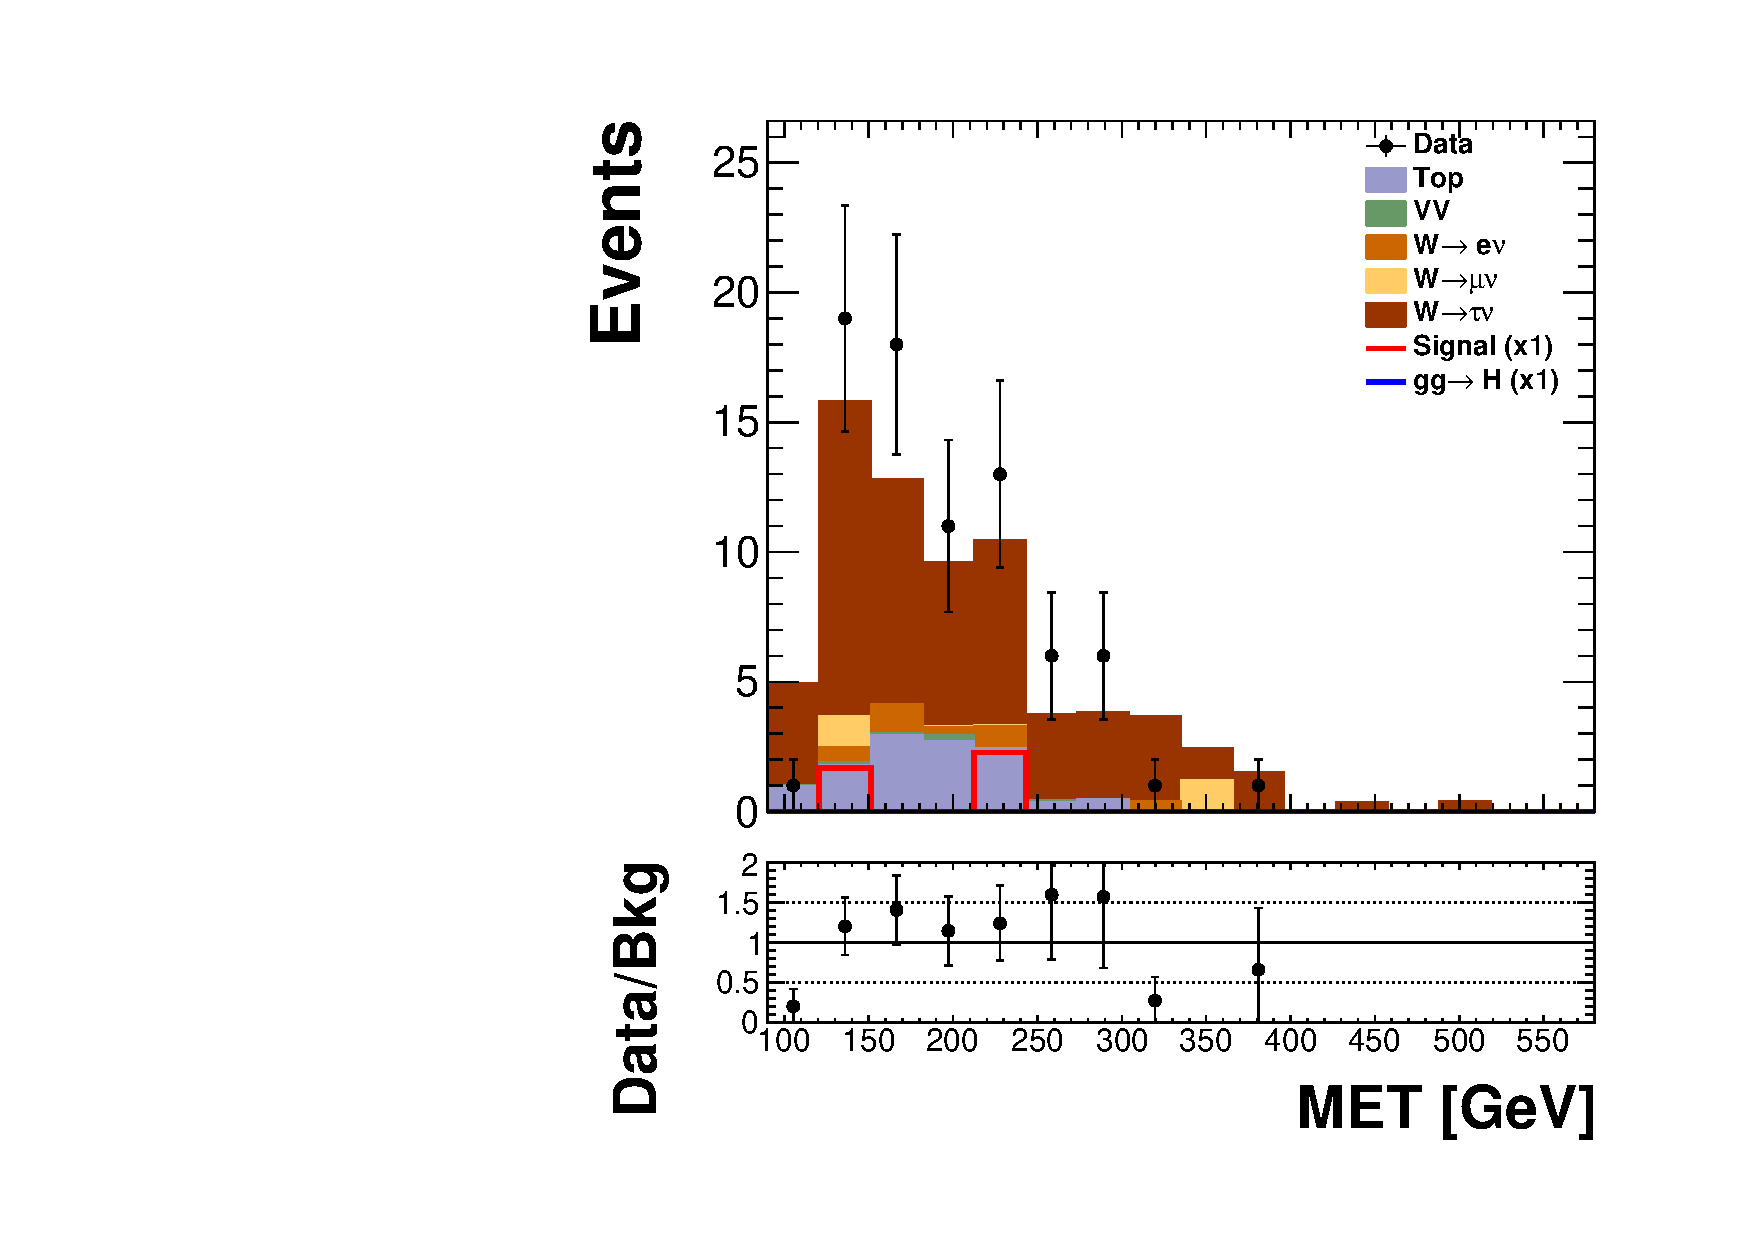
\includegraphics[width=.45\textwidth]{Chapter07/CrossCheck/Wtaunu/sigWta_metNoMuon.pdf}}
\caption[MET for the $W\rightarrow e\nu$, $W\rightarrow\mu\nu$ and $W\rightarrow\tau\nu$ control regions obtained with the cross check analysis.]
{\gls{MET} for the (a) $W\rightarrow e\nu$, (b) $W\rightarrow\mu\nu$ and (c) $W\rightarrow\tau\nu$ control regions obtained with the cross check analysis.}
\label{FIGURE:ParkedDataAnalysis_WBackground_MetNoMu}
\end{figure}

\begin{figure}[!htb]
\centering
\subfloat[]{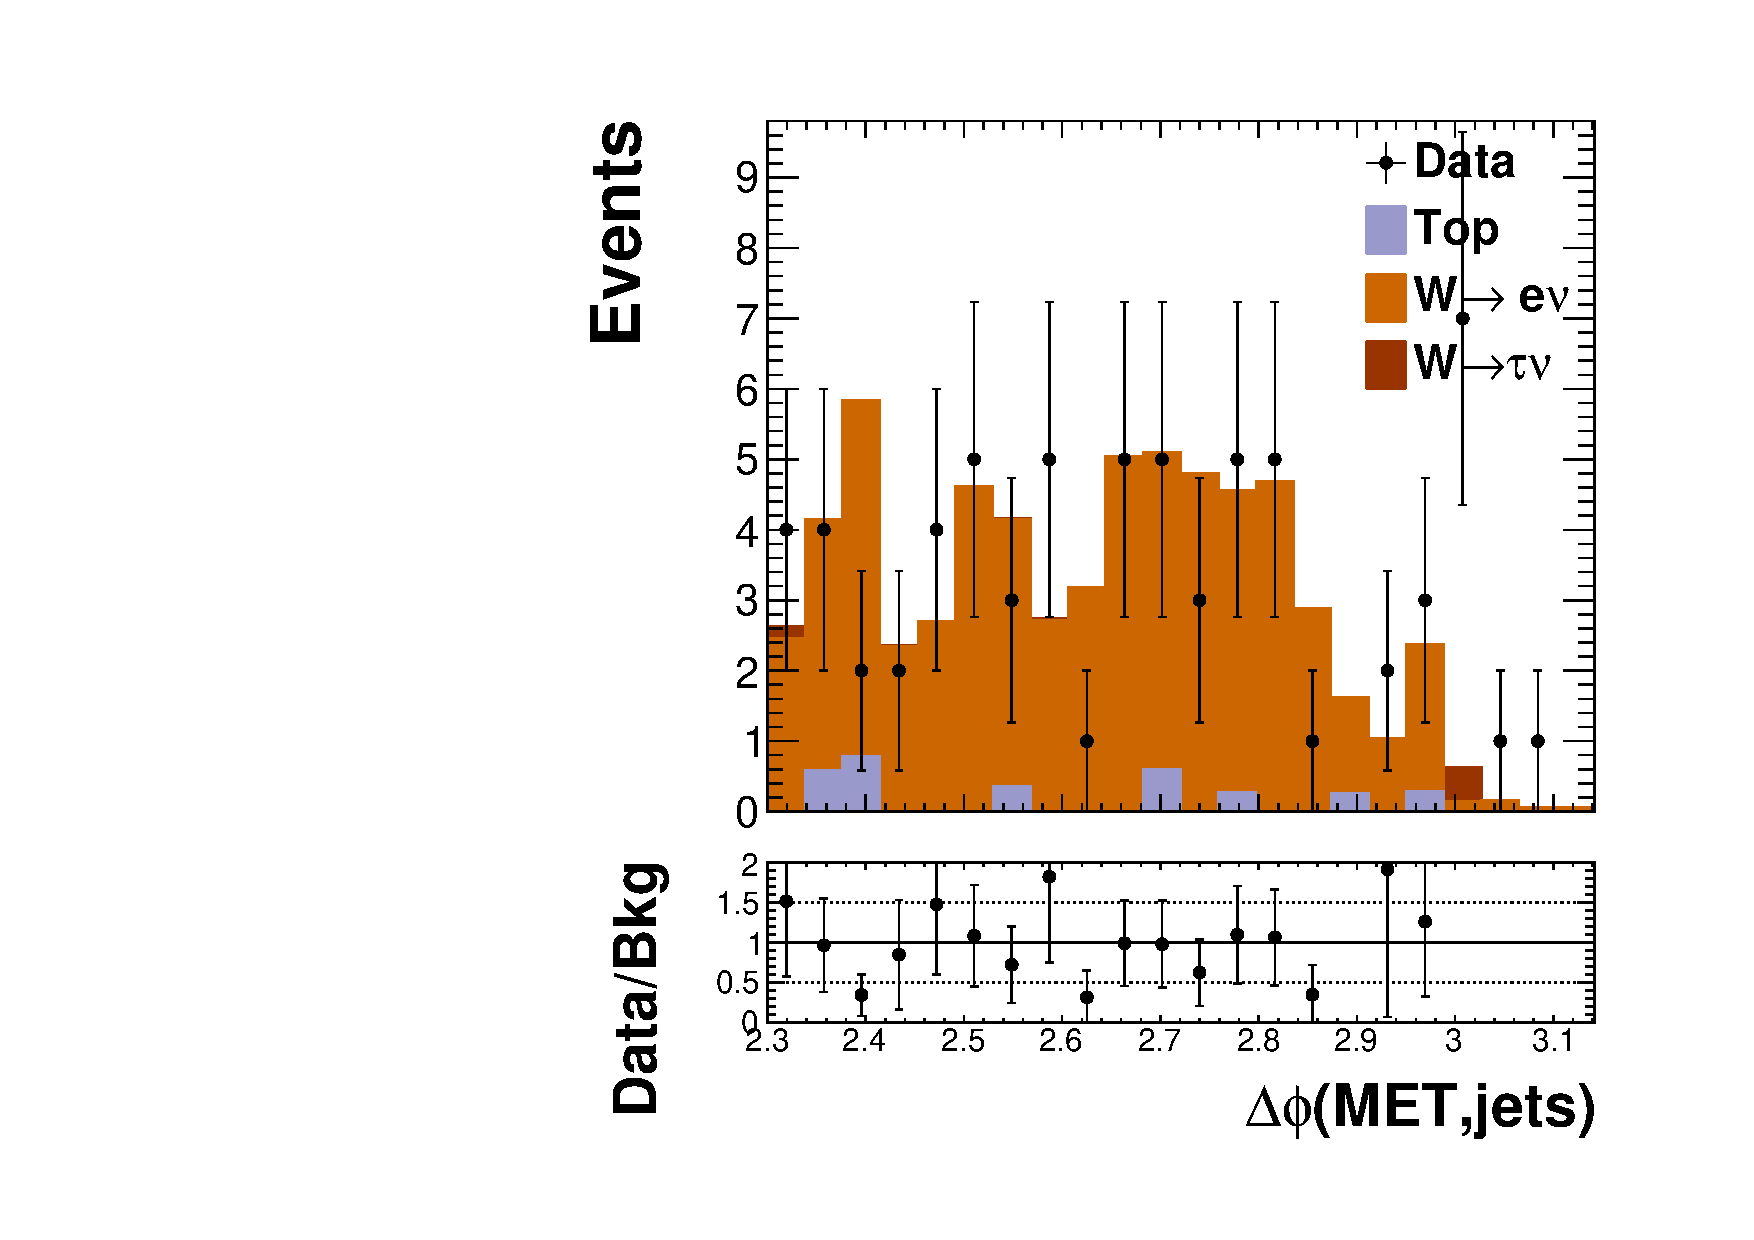
\includegraphics[width=.45\textwidth]{Chapter07/CrossCheck/Wenu/sigWel_MinDeltaPhiMetAllJets.pdf}}
\subfloat[]{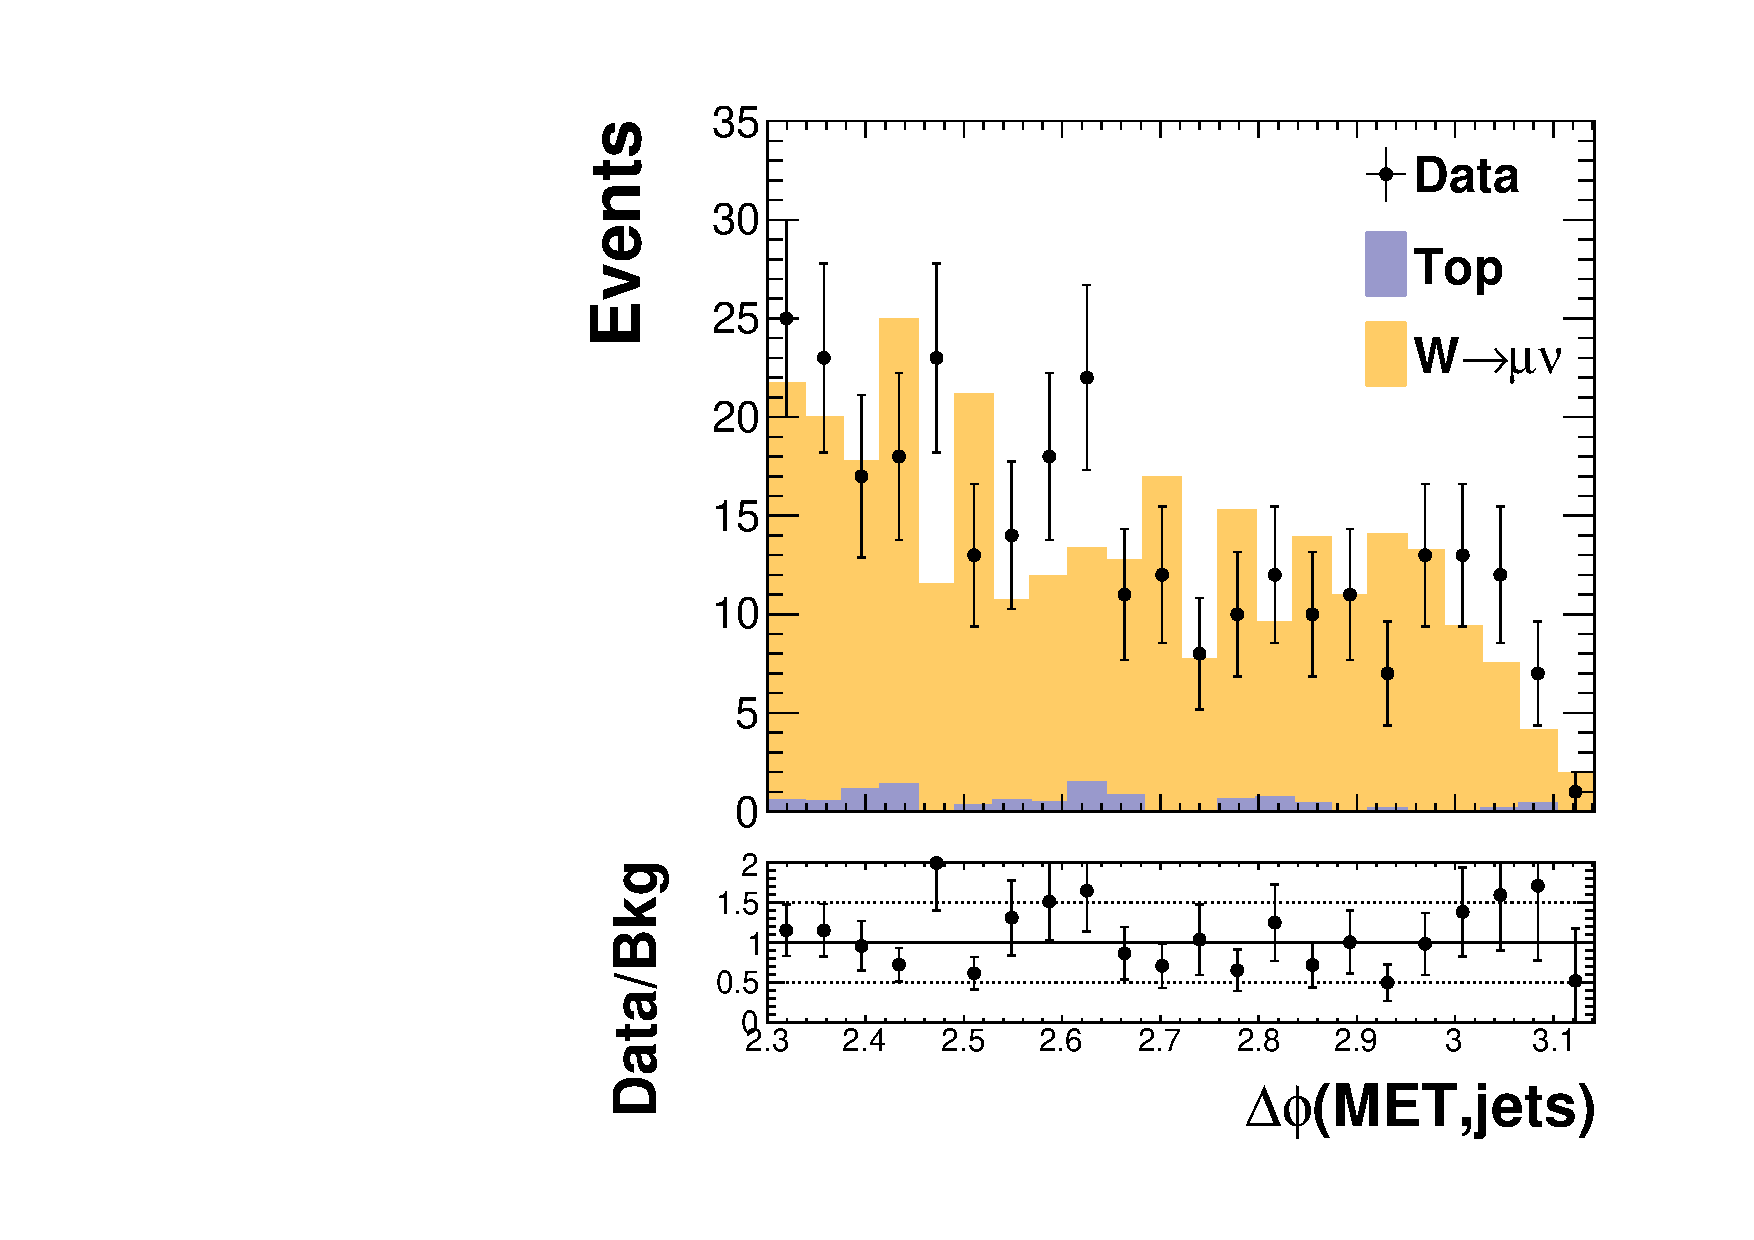
\includegraphics[width=.45\textwidth]{Chapter07/CrossCheck/Wmunu/sigWmu_MinDeltaPhiMetAllJets.pdf}} \\
\subfloat[]{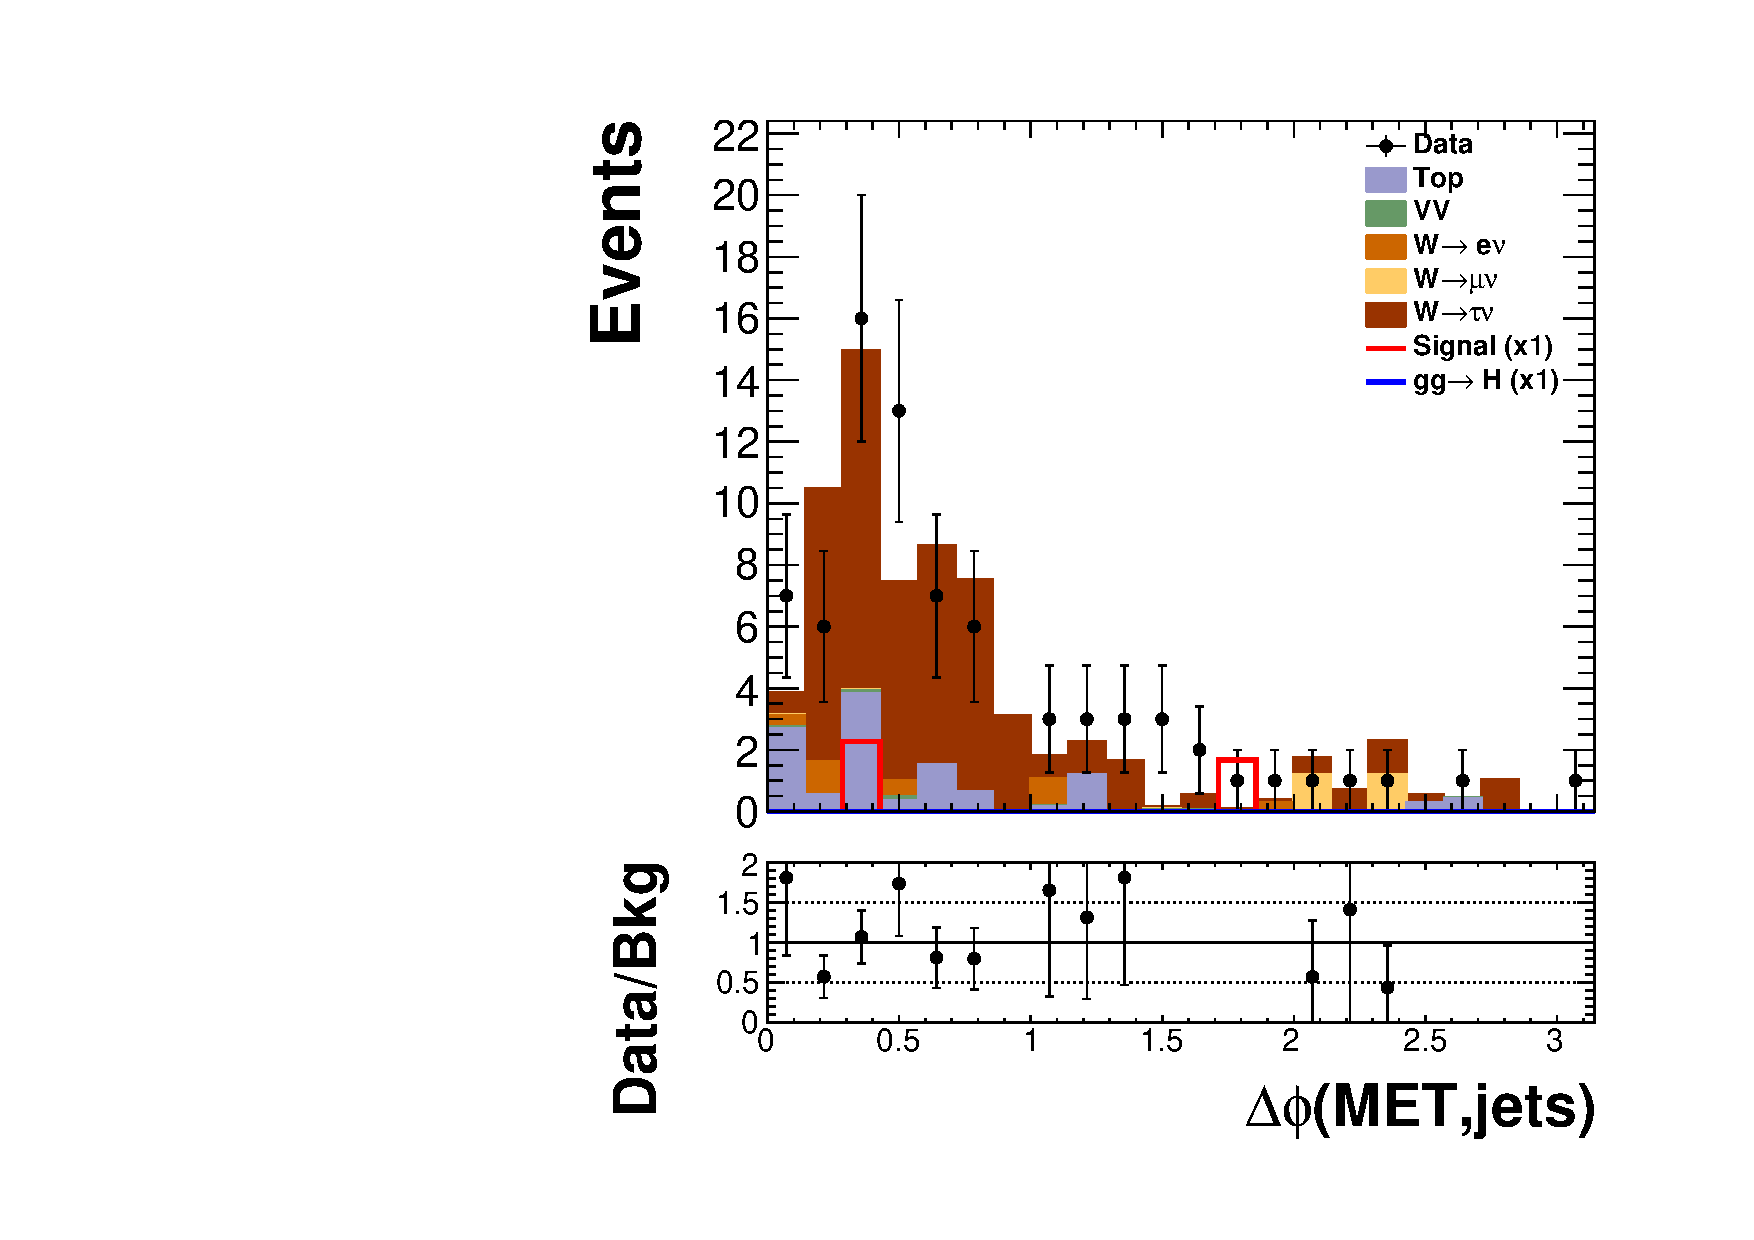
\includegraphics[width=.45\textwidth]{Chapter07/CrossCheck/Wtaunu/sigWta_MinDeltaPhiMetAllJets.pdf}}
\caption[Minimum azimuthal angle separation between any jet with $p_{T}>30\,\GeV$ and the MET $\Delta\phi(\text{MET},jets)$ for the $W\rightarrow e\nu$, $W\rightarrow\mu\nu$ and $W\rightarrow\tau\nu$ control region obtained with the cross check analysis.]
{Minimum azimuthal angle separation between any jet with $p_{T}>30\,\GeV$ and the \gls{MET} $\Delta\phi(\text{MET},jets)$ for the (a) $W\rightarrow e\nu$, (b) $W\rightarrow\mu\nu$ and (c) $W\rightarrow\tau\nu$ control region obtained with the cross check analysis.}
\label{FIGURE:ParkedDataAnalysis_WBackground_MinDeltaPhi}
\end{figure}

All presented distributions show good agreement between data and \gls{MC} simulation. The event yields in each control region for both data and \gls{MC} simulation and the final estimations of the W$\rightarrow l\nu$ backgrounds in the signal region can be found in table \ref{TABLE:ParkedDataAnalysis_WBackground_Summary}.
 
% \begin{table}[!htb]
% \centering
% \begin{tabular}{|l|c|c|c|}
% \hline
%  & W$\rightarrow$e$\nu$ & W$\rightarrow\mu\nu$ & W$\rightarrow\tau\nu$ \\
% \hline\hline
% $N_{C}^{data}$ &    $68\pm8.2$ &   $300\pm17.3$ &    $76\pm8.7$ \\
% $N_{C}^{bkg}$  &   $3.5\pm1.2$ &  $14.8\pm2.5$  &  $13.3\pm2.8$ \\
% $N_{C}^{MC}$   & $128.0\pm8.0$ & $399.9\pm14.9$ &  $80.8\pm6.4$ \\
% $N_{S}^{MC}$   & $114.9\pm8.9$ & $143.7\pm10.2$ & $121.9\pm8.7$ \\
% \hline\hline
% SF             & $0.50\pm0.06\pm0.03$ & $0.71\pm0.04\pm0.03$ & $0.78\pm0.11\pm0.07$ \\
% \hline\hline
% $N_{S}$        & $57.9\pm7.4\pm7.7$ & $102.5\pm6.2\pm11.7$ & $94.6\pm13.1\pm23.8$ \\
% \hline
% \end{tabular}
% \caption{Summary of the W background estimates. The quoted uncertainties are of statistical origin. Systematic uncertainties are shown, as well, for SF and $N_S$. The systematic uncertainty given for SF contains only the \gls{MC} statistics, whereas for $N_{S}$ it represents the full systematic are shown \cite{ARTICLE:CMSVBFHiggsInvisibleParkedAnalysisPAS}.}
% \label{TABLE:ParkedDataAnalysis_WBackground_Summary}
% \end{table}

\begin{table}[!htb]
\centering
\begin{tabular}{|l|c|c|c|}
\hline
 & W$\rightarrow$e$\nu$ & W$\rightarrow\mu\nu$ & W$\rightarrow\tau\nu$ \\
\hline\hline
$N_{C}^{data}$ & $  68 \pm 8.2$ & $300   \pm 17.3$ & $76  \pm 8.7$ \\
$N_{C}^{bkg}$  & $ 6.4 \pm 1.5$ & $19.3  \pm  2.4$ & $23.9\pm 3.6$ \\
$N_{C}^{MC}$   & $87.3 \pm 7.7$ & $227.6 \pm 12.0$ & $60.3\pm 6.0$ \\
$N_{S}^{MC}$   & $90.3 \pm 8.7$ & $119.9 \pm  9.9$ & $94.0\pm 8.5$ \\
\hline\hline               
SF             & $0.71\pm0.11$ & $1.23\pm0.10$   & $0.86\pm0.18$ \\
\hline\hline
$N_{S}$        & $63.8\pm12.0$ & $147.9\pm 17.2$ & $81.2\pm18.3$ \\
\hline
\end{tabular}
\caption[Summary of the W background estimates as calculated by the cross check analysis.]
{Summary of the W background estimates as calculated by the cross check analysis. The quoted uncertainties are of statistical origin.}
\label{TABLE:ParkedDataAnalysis_WBackground_Summary}
\end{table}

The cross check analysis has determined exactly the same data event yields for all W control selection regions. However, some discrepancies were observed in the \gls{MC} simulation yields possibly pointing to a problem with the weighting of events.

\clearpage

%%%%%%%%%%%%%%%%%%%%%%%%%%%%%%%%%%%%%%%%%%%%%%%%%%%%%%%%%%%%%%%%%%%%%%%%%%%%%%%%%%%%
%%% SUBSECTION
%%%%%%%%%%%%%%%%%%%%%%%%%%%%%%%%%%%%%%%%%%%%%%%%%%%%%%%%%%%%%%%%%%%%%%%%%%%%%%%%%%%%
\subsection{Top background estimation}
\label{SECTION:ParkedDataAnalysis_ControlRegions_TopBackground}

%Status: DONE (reviewed J.Pela x1)

%TODO: Wrong definition of region 1 in the article
To estimate the contribution of processes involving the top quark in the signal region, two control regions were defined. The first region is the same as the one used for the signal region with the exception that the lepton vetoes are replaced by selecting two tight leptons, exactly one tight electron and one tight muon and no other additional leptons. The $\Delta\phi(\text{MET},jets)$ is not performed to increase statistics.  This region is found to be composed almost entirely of $t\bar{t}$ events. The data event yield in this region was determined to be 21 events, by both main and cross check analysis. The data-to-simulation scale factor obtained is $1.21\pm 0.19$ (data stat.)$ \pm 0.16 $(syst.).

%TODO: Not in the analysis note, how was this combined into the final result?
A second region selects events with same criteria as the signal region with the exception that the lepton vetoes are replaced by selecting a single tight lepton (e or $\mu$) and no other additional leptons. Additionally, one of the leading jets is required to be identified as a jet from a b quark (using the Combined Secondary Vertex algorithm \cite{ARTICLE:CMSIdentificationOfbQuarks}). The composition of this region was determined to be 10\% single top, 50\% $t\bar{t}$ and 40\% W+jets using \gls{MC} simulation. For this region the main analysis observed 429 events which lead to a data-to-simulation scale factor of $0.88\pm 0.07$ (data stat.)$ \pm 0.08$ (syst.). The systematic uncertainties associated with the determined scale factors are dominated by the small statistics available in \gls{MC} simulation. Taking into account these results, a 20\% systematic uncertainty is assigned to the top quark contribution to the signal region. 

%%%%%%%%%%%%%%%%%%%%%%%%%%%%%%%%%%%%%%%%%%%%%%%%%%%%%%%%%%%%%%%%%%%%%%%%%%%%%%%%%%%%
%%% SUBSECTION
%%%%%%%%%%%%%%%%%%%%%%%%%%%%%%%%%%%%%%%%%%%%%%%%%%%%%%%%%%%%%%%%%%%%%%%%%%%%%%%%%%%%
\subsection{QCD background estimation}
\label{SECTION:ParkedDataAnalysis_ControlRegions_QCDBackground}

%Status: DONE (reviewed J.Pela x1)

%TODO: What shape?
The contribution of \gls{QCD} multi-jet processes is determined with a data-driven method using non-isolated \gls{MET}. Three regions are defined: Region I is denoted as ``inverted'' and gives the description of the \gls{QCD} multi-jet shape; Region II is denoted as ``3-jet'' where a cross check is preformed to see how well the \gls{QCD} multi-jet shapes are described; and Region III is denoted as ``sideband'' in this region the normalization of the \gls{QCD} multi-jet shapes is extracted to apply to the signal region.

% QCD Shape region
The \gls{QCD} multi-jet \textit{inverted region}, is selected by changing the $\Delta\phi(\text{MET},jets)$ requirement to $min(\Delta\phi(\text{MET}),jets)<1.0$ while requiring $\Delta\phi(\text{MET},jet_{1,2})>2.3$. The change in requirements provides two leading jets which are signal-like, but at the same time ensures \gls{MET} will not be isolated. The distribution of $\text{MET}_{sig}$ in the inverted region is shown in figure \ref{FIGURE:ParkedDataAnalysis_QCDBackground_Plots}. The selected events in this region are expected to originate about 20\% from W, Z and top processes. The \gls{QCD} shape is defined as the shape observed in data after the subtraction of non-\gls{QCD} backgrounds, which are normalised by scale factors determined in their respective control regions, but with the same inverted selection. Good agreement between data and the \gls{VBF} enriched \gls{QCD} \gls{MC} simulation in this region is observed as shown in figure \ref{FIGURE:ParkedDataAnalysis_QCDBackground_Plots}.

% TODO: NOT IN THE AN!!! is it norm 3?
The \textit{3-jet region} is defined by requiring $\Delta\phi(\text{MET},jets)>1.0$, $\text{MET}_{sig}>3$ and at least three jets with p$_{T}>30\,\GeV$. Using \gls{MC} simulation the contribution from signal to this region was determined to be negligible. This region is used to ensure that the \gls{QCD} shape is adequate. The expected number of \gls{QCD} events in the \textit{3-jet region}, n$_{QCD}^{3j}$, is the data yield in this region subtracted from backgrounds with the W and Z predictions being normalised to their control leptonic regions. The \gls{QCD} shape can now be compared between the data in this region and the \textit{inverted region} with $\Delta\phi(\text{MET},jet_{1,2})>1.0$ and normalizing it to n$_{QCD}^{3j}$. The distribution of $\text{MET}_{sig}$ in the \textit{3-jet region} is shown in figure \ref{FIGURE:ParkedDataAnalysis_QCDBackground_Plots}. The discrepancy between data and the prediction is found to be less than 20\%. Unfortunately, since most of the events in the signal region will only have two jets, this control region cannot be used for the final \gls{QCD} multi-jet estimation.

\begin{figure}[!htb]
\centering
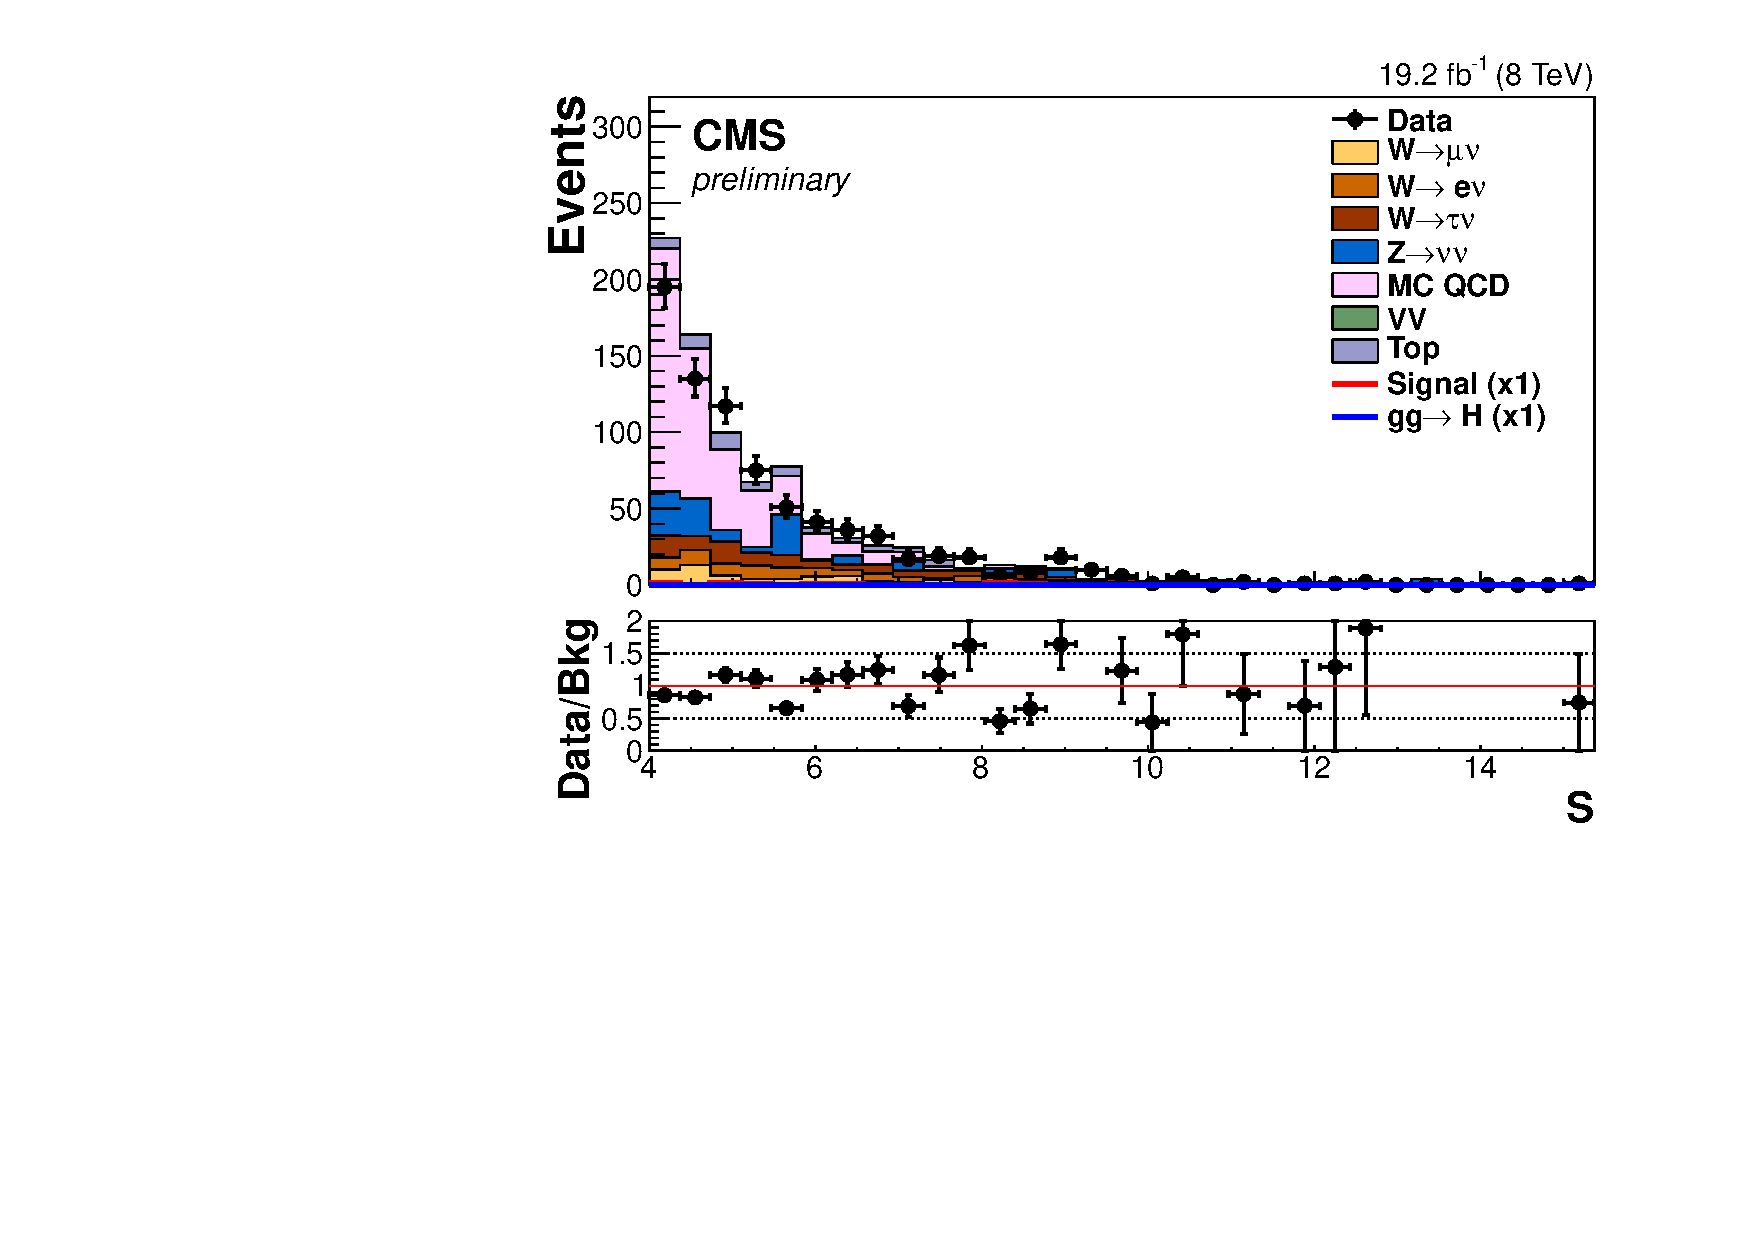
\includegraphics[width=.45\textwidth]{Chapter07/Images/output_invqcd_qcd_metnomu_significance.pdf}
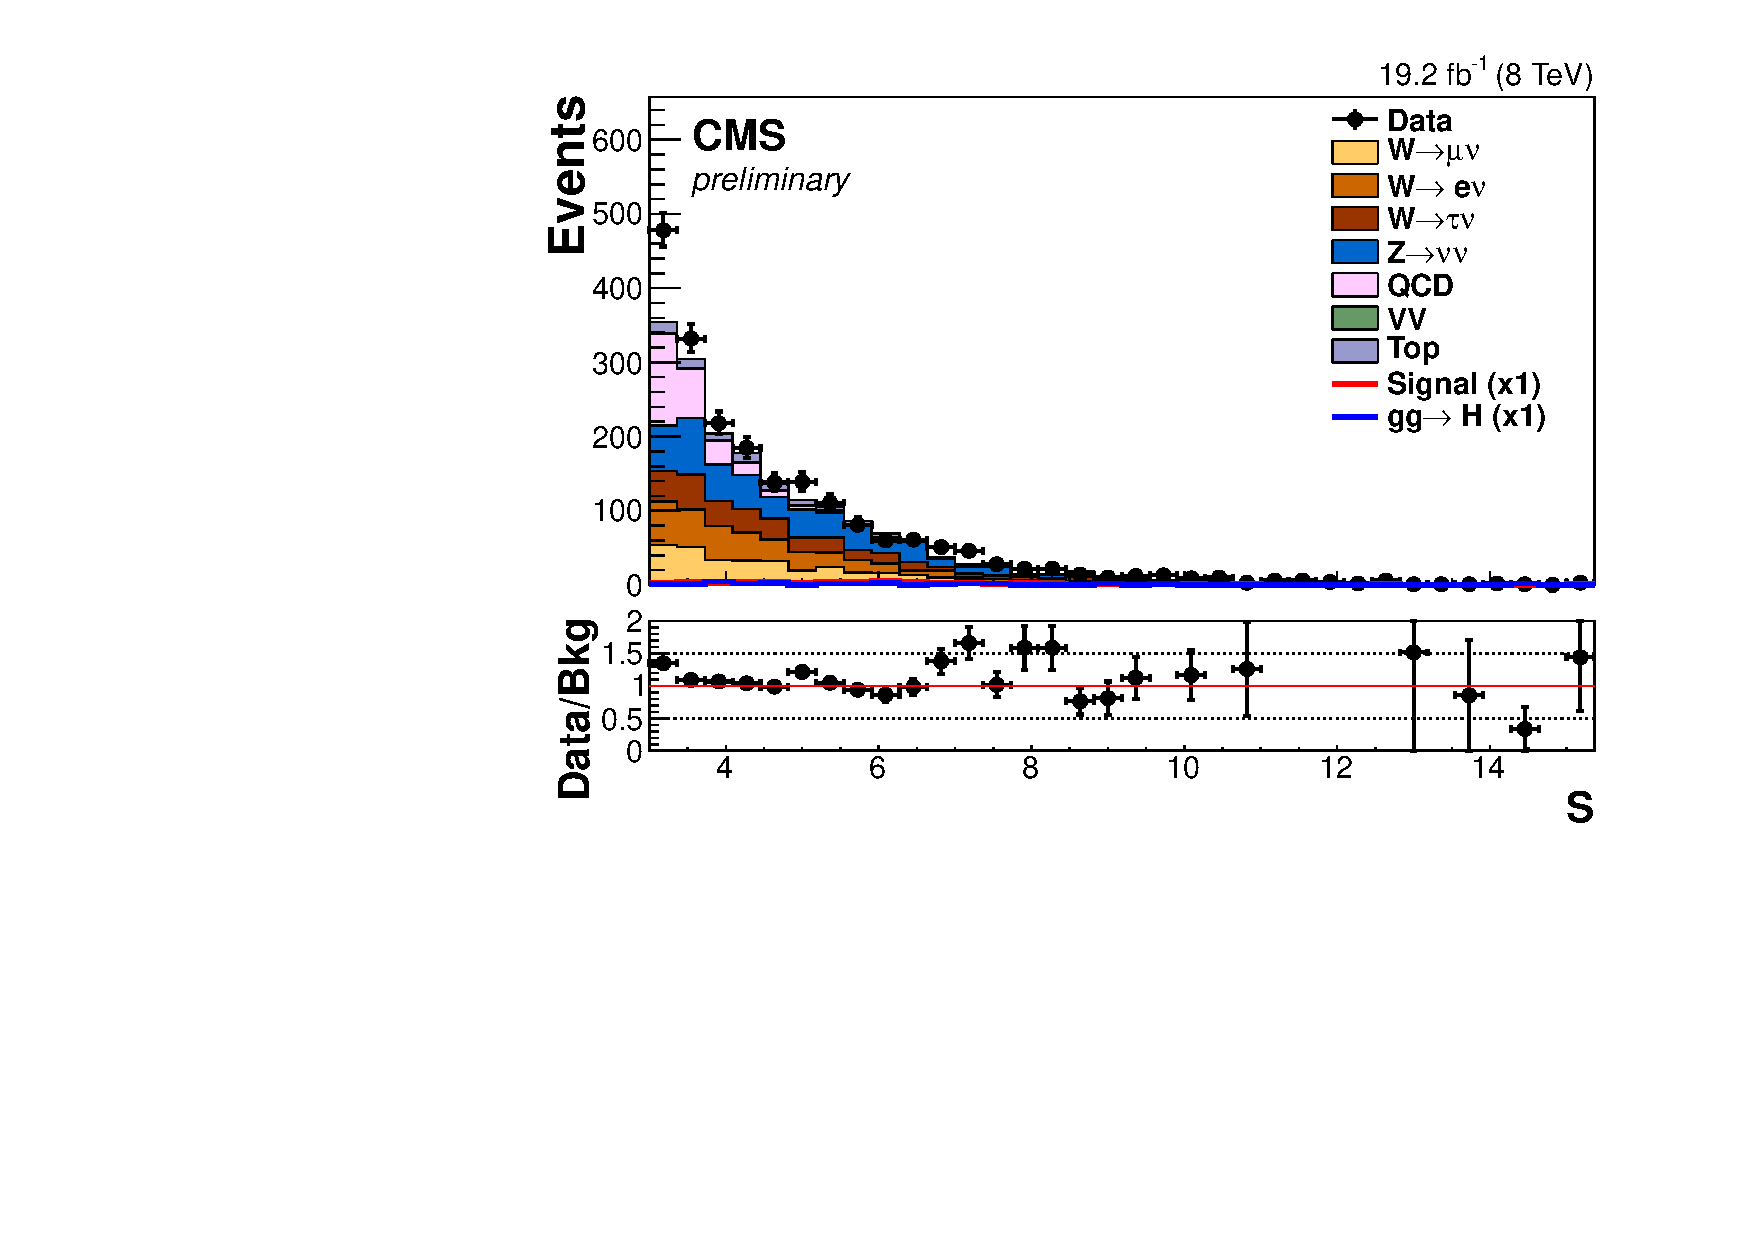
\includegraphics[width=.45\textwidth]{Chapter07/Images/output_invqcd_3j_nunu_metnomu_significance.pdf}
\caption[\MET significance $\text{MET}_{sig}$ for events with $\Delta\phi(\text{MET},jets)<1.0$ and $\Delta\phi(\text{MET},jet_{1,2})>2.3$. MET significance, $\text{MET}_{sig}$, for events with $\Delta\phi(\text{MET},jets)>1.0$ and at least 3 jets with $p_T>30\,\GeV$.]
{(left) \MET significance $\text{MET}_{sig}$ for events with $\Delta\phi(\text{MET},jets)<1.0$ and $\Delta\phi(\text{MET},jet_{1,2})>2.3$. MC QCD is the \gls{QCD} \gls{MC} normalised to the background-subtracted data yield. (right) \gls{MET} significance, $\text{MET}_{sig}$, for events with $\Delta\phi(\text{MET},jets)>1.0$ and at least 3 jets with $p_T>30\,\GeV$. The \gls{QCD} is modelled by data using the inverted $\Delta\phi(\text{MET},jets)<1.0$ and $\Delta\phi(\text{MET},jet_{1,2})>1$ selection, after background subtraction, and normalised to the background-subtracted data yield. In both figures, the W and Z backgrounds have been normalised to their respective control regions in the same conditions. The last bin represents all those events falling above the range of the histogram~\cite{ARTICLE:CMSVBFHiggsInvisibleParkedAnalysisPAS}.}
\label{FIGURE:ParkedDataAnalysis_QCDBackground_Plots}
\end{figure}

% NORM 1 
%TODO: What happens to the all mindeltaphi cut??? Is it extrapolated shape????
The \textit{sideband region} is used to determine the normalization of the \gls{QCD} shape to be used in the signal region. This region is defined by selecting events with $3<\text{MET}_{sig}<4$ and $1.0<\Delta\phi(\text{MET},jet_{1,2})<2.0$. In this region it is observed that the normalisation factor decreases rapidly with increasing requirements as a function of $\text{MET}_{sig}$ and as a function of $\Delta\phi(\text{MET},jet_{1,2})$. This normalization factor variation is fitted and extrapolated to the signal region requirements. The average of the two extrapolation factors is used as the central prediction and the envelope is used to assign the systematic uncertainty on the \gls{QCD} multi-jets normalisation.

%%%%%%%%%%%%%%%%%%%%%%%%%%%%%%%%%%%%%%%%%%%%%%%%%%%%%%%%%%%%%%%%%%%%%%%%%%%%%%%%%%%%
%%% SECTION
%%%%%%%%%%%%%%%%%%%%%%%%%%%%%%%%%%%%%%%%%%%%%%%%%%%%%%%%%%%%%%%%%%%%%%%%%%%%%%%%%%%%
\section{Systematics}

%Status: DONE (reviewed J.Pela x1)

The dominant source of uncertainty are the statistical uncertainties associated with the yields of the control regions both in data and \gls{MC} simulation, which are used for the estimation of the different backgrounds in the signal region. 

The errors associated with jet energy scale, unclustered energy scale and jet energy resolution are estimated for both signal and background processes by varying each quantity independently by its uncertainties \cite{ARTICLE:CMSDeterminationJetEnergyCalibration}. For each variation, the \gls{MET} is recomputed and the signal and background predictions are recalculated. A similar procedure is applied for the lepton efficiency and \gls{PU} scale factors which are applied to the \gls{MC} simulation, which are also varied by their uncertainties and propagated through the analysis \cite{ARTICLE:CMSMuonReconstruction7TeV,ARTICLE:CMSElectronReconstruction8TeV}.

The uncertainty associated with the integrated luminosity measurement is of 2.6\% and is only applied to the \gls{MC} simulated signal and backgrounds \cite{ARTICLE:CMSLuminosityBasedonPixelClusterCounting}. The main backgrounds are normalised using a data-driven method which takes into account the trigger efficiency, while the impact of the luminosity measurement in the signal and minor backgrounds was found to be negligible.

Uncertainties associated with diboson cross sections are taken from \gls{CMS} measurements \cite{ARTICLE:CMSMeasurmentOfWWandZZxsec}, while the theoretical uncertainties due to \gls{PDF} and \gls{QCD} scales associated to the signal cross section are taken from the \gls{LHC} Higgs Cross Section Working Groups Yellow Report 3 \cite{ARTICLE:HandbookofLHCHiggsCrossSectionsInclusiveObservables,ARTICLE:HandbookofLHCHiggsCrossSectionsDifferentialDistributions}.

% TODO: Ask patrick, ``compatible within statistical uncertainty`` of what?
The uncertainty on the extrapolation of the  $Z\rightarrow\nu\nu$ background was obtained by comparing the \gls{QCD} produced $Z/\gamma^{*}\rightarrow\mu\mu$ prediction from \textsc{MADGRAPH} and a\textsc{MC@NLO\_MG5} \cite{ARTICLE:aMCatNLO}.

The results from both generators were compatible within statistical uncertainty, leading to no additional uncertainties being added. 

Table \ref{TABLE:ParkedDataAnalysis_Systematics_Summary} shows a summary of the overall size of each uncertainty as a percentage of the total signal and background predictions.

\begin{table}[!htb]
\centering
\begin{tabular}{|l|c|c|}
\hline 
Source                                            & Total background &     Signal \\
\hline\hline
Control region data statistics                     &            9.3  &          - \\
MC statistics                                      &            5.4  &        3.8 \\
Jet energy scale                                   &            4.6  &         11 \\
$W\rightarrow\tau\nu$ control region extrapolation &            4.3  &          - \\
QCD normalisation                                  &            3.2  &          - \\
Jet energy resolution                              &            3.0  &        1.8 \\
Lepton ID efficiency                               &            2.4  &          - \\
Unclustered energy scale                           &            1.9  &        1.6 \\
Pileup weight                                      &            1.1  &        1.5 \\
Top MC scale factor uncertainties                  &            0.25 &          - \\
Luminosity                                         &            0.02 &        2.6 \\
QCD scale, PDF and cross section uncertainties     &            0.01 &        5.2 \\
\hline
\end{tabular}
\caption[Summary of the uncertainties on the total background and signal yields.]
{Summary of the uncertainties on the total background and signal yields. All uncertainties affect the normalization of the yield, and are quoted as the change in \% in the total background or signal estimate, when each systematic effect is varied according to its uncertainties. The signal uncertainties are given for $m_H=125\,\GeV$ and $\BRinv=100$\%~\cite{ARTICLE:CMSVBFHiggsInvisibleParkedAnalysisPAS}.}
\label{TABLE:ParkedDataAnalysis_Systematics_Summary}
\end{table}

%%%%%%%%%%%%%%%%%%%%%%%%%%%%%%%%%%%%%%%%%%%%%%%%%%%%%%%%%%%%%%%%%%%%%%%%%%%%%%%%%%%%
%%% SECTION
%%%%%%%%%%%%%%%%%%%%%%%%%%%%%%%%%%%%%%%%%%%%%%%%%%%%%%%%%%%%%%%%%%%%%%%%%%%%%%%%%%%%
\section{Results}

%Status: DONE (reviewed J.Pela x1)

The final estimations of the number of events predicted in the signal region are derived using scale factors determined with \gls{MC} simulation for the W, Z where data control regions are used to normalise the predictions. In the case of the \gls{QCD} multi-jet background the contribution to the signal region is determined using non-isolated \gls{MET} events. The remaining backgrounds are estimated directly from \gls{MC} simulation. These results are summarized in table \ref{TABLE:ParkedDataAnalysis_Results_Summary} for both the main and the cross check analysis.

% New numbers cross check
% Signal Region - Top     : 5.02825+/-1.21163
% Signal Region - VV      : total: 3.5+/-0.5  ZZ: 0.717446 +/- 0.153554 WW: 0.68089 +/- 0.249246 WZ: 2.13829 +/- 0.365195
% Signal Region - Sig VBF : 267.7 +/- 9.1 (stat) 
% Signal Region - Sig ggH :  21.7 +/- 6.0 (stat) 

% Region Signal - Data       : 508 +/- 22.5389
% Region Signal - W total    : 304.22 +/- 15.66
% Region Signal - W electron : 90.3453 +/- 8.65291
% Region Signal - W muon     : 119.9 +/- 9.90557
% Region Signal - W tau      : 93.9741 +/- 8.49958
% Region Signal - VV         : 3.5 \pm 0.7      %<------ Missing events
% Region Signal - Z          : 227.06 +/- 8.60235
% Region Signal - Z QCD      : 226.689 +/- 8.60223
% Region Signal - Z EWK      : 0.371393 +/- 0.0471477
% Region Signal - Top        : 5.02825 +/- 1.21163
% Region Signal - QCD Inc    : 
% Region Signal - QCD VBF    : 17.2975 +/- 2.80396
% Region Signal - Sig VBF    : 267.715 +/- 9.12686
% Region Signal - Sig ggH    : 21.7152 +/- 5.989

% Region Zmumu  - Data       : 18 +/- 4.24264 (stat) 
% Region Zmumu  - Z total    : 16.1181 +/- 1.85029 (stat)  100.0%
% Region Zmumu  - Z QCD      : 11.1848 +/- 1.84217 (stat)   69.3%
% Region Zmumu  - Z EWK      : 4.93329 +/- 0.173201 (stat)  30.6%
% Region Zmumu  - VV         : 0.141569 +/- 0.103953 (stat) 
% Region Zmumu  - Top        : 0 +/- 0
% Region Zmumu  - W          : 0 +/- 0
% Region Zmumu  - QCD        : 0 +/- 0
% Region Zmumu  - QCD VBF    : 0 +/- 0
% Region Signal - XSec Ratio : 5.651 +/- 0.023 = B
% Region Signal - Eff  Ratio : (1.8 +/- 0.1)x10e-6 / (1.2 +/- 0.1)x10e-6 = 1.5 +/- 0.15 = A 
% Region Signal - Z in CR    : N_data - N_bkg = 17.86 +/- 4.2439133 = N
% Region Signal - Prediction : N * A * B = 151.38 +/- 39.0

% Region Elec+MET - Data     : 68 +/- 8.24621
% Region Elec+MET - Z total  : 2.22283 +/- 0.710462
% Region Elec+MET - Z QCD    : 1.87763 +/- 0.709008
% Region Elec+MET - Z EWK    : 0.345203 +/- 0.0454355
% Region Elec+MET - VV       : 0.286811 +/- 0.146591
% Region Elec+MET - Top      : 3.14804 +/- 1.17516
% Region Elec+MET - W        : 87.9693 +/- 7.69928
% Region Elec+MET - W elec   : 87.249 +/- 7.68202
% Region Elec+MET - W muon   : 0.0104352 +/- 0.0104352
% Region Elec+MET - W tau    : 0.709861 +/- 0.51503
% Region Control  - QCD      : - error
% Region Control  - QCD VBF  : 
% Region Control  - other    : 

% Region Muon+MET - Data     : 300 +/- 17.3205
% Region Muon+MET - Z total  : 7.87255 +/- 1.34697
% Region Muon+MET - Z QCD    : 6.05375 +/- 1.34284
% Region Muon+MET - Z EWK    : 1.8188 +/- 0.10535
% Region Muon+MET - VV       : 1.57188 +/- 0.38315
% Region Muon+MET - Top      : 9.87987 +/- 1.90302
% Region Muon+MET - W        : 227.56 +/- 12.0924
% Region Muon+MET - W elec   : 0 +/- 0
% Region Muon+MET - W muon   : 227.56 +/- 12.0924
% Region Muon+MET - W tau    : 0 +/- 0
% Region Muon+MET - QCD      : 0 +/- 0
% Region Muon+MET - QCD VBF  : 5.21448 +/- 1.54598
% Region Control  - other    : 19.3243 +/- 2.3627563
% Region Control  - SF       :
% Region Signal - Prediction :

% Region Tau+MET  - Data     : 76 +/- 8.7178
% Region Tau+MET  - Z total  : 5.96052 +/- 1.17232
% Region Tau+MET  - Z QCD    : 5.49888 +/- 1.17117
% Region Tau+MET  - Z EWK    : 0.46164 +/- 0.0518545
% Region Tau+MET  - VV       : 0.503659 +/- 0.194011
% Region Tau+MET  - Top      : 11.7464 +/- 2.66666
% Region Tau+MET  - W        : 66.0068 +/- 6.3966
% Region Tau+MET  - W elec   : 3.20246 +/- 1.34404
% Region Tau+MET  - W muon   : 2.4896 +/- 1.69115
% Region Tau+MET  - W tau    : 60.3148 +/- 6.0208
% Region Tau+MET  - QCD      :  0 +/- 0
% Region Tau+MET  - QCD VBF  :  0.551827 +/- 0.495551
% Region Control  - other    : 
% Region Control  - SF       :
% Region Signal - Prediction :

\begin{table}[!htb]
\centering
\begin{tabular}{|l|c|c|c|}
\hline 
        & \multicolumn{3}{c|}{Event yields} \\
\hline
Process               & Main                      & Cross Check       & Difference [\%] \\
\hline\hline
$Z\rightarrow\nu\nu$  & $158.1 \pm 37.3 \pm 21.2$ & $151.4 \pm 39.0$  &           -4.25 \\
$W\rightarrow e\nu$   & $ 57.9 \pm 7.4  \pm  7.7$ &  $63.8 \pm 12.0$  &           +10.2 \\
$W\rightarrow\mu\nu$  & $102.5 \pm 6.2  \pm 11.7$ & $147.9 \pm 17.2$  &           +43.4 \\
$W\rightarrow\tau\nu$ & $ 94.6 \pm 13.1 \pm 23.8$ &  $81.3 \pm 18.3$  &           -14.1 \\
top                   & $  5.5 \pm 1.8$           &   $5.0 \pm 1.2$   &            -9.1 \\ 
VV                    & $  3.9 \pm 0.7$           &   $3.5 \pm 0.7$   &           -10.3 \\  
QCD multijet          & $   17 \pm 14$            &                -  &               - \\
\hline\hline                                                     
Total Background      & $439.4 \pm 40.7 \pm 43.5$ &   $452.9\pm47.93$ &            +3.0 \\
\hline\hline                                                     
Signal(VBF)           & $273.1 \pm 31.2 $         &   $267.7 \pm 9.1$ &            -2.0 \\
Signal(ggH)           & $ 23.1 \pm 15.9 $         &   $ 21.7 \pm 6.0$ &            -6.1 \\
\hline\hline                                                     
Observed data         & 508                       &               508 &             0.0 \\
\hline
\end{tabular}
\caption[Summary of the estimated number of background and signal events, together with the observed yield, in the VBF search signal region.]
{Summary of the estimated number of background and signal events, together with the observed yield, in the \gls{VBF} search signal region. The signal yield is given for $m_H=125\,\GeV$ and $\BRinv=100$\%. For the main analysis, where two errors quoted, they are the statistical and systematic uncertainties respectively, where only one is quoted it is the systematic uncertainty~\cite{ARTICLE:CMSVBFHiggsInvisibleParkedAnalysisPAS}. For the cross check analysis only statistical errors are quoted.}
\label{TABLE:ParkedDataAnalysis_Results_Summary}
\end{table}

Distributions of the $\Delta\eta_{jj}$, $M_{jj}$, $\text{MET}_{sig}$ and \gls{MET} variables, in the signal region, are shown in figure \ref{FIGURE:ParkedDataAnalysis_Results_SigRegPlots}. 

% Cross Check
\begin{figure}[!htb]
\centering
\subfloat[]{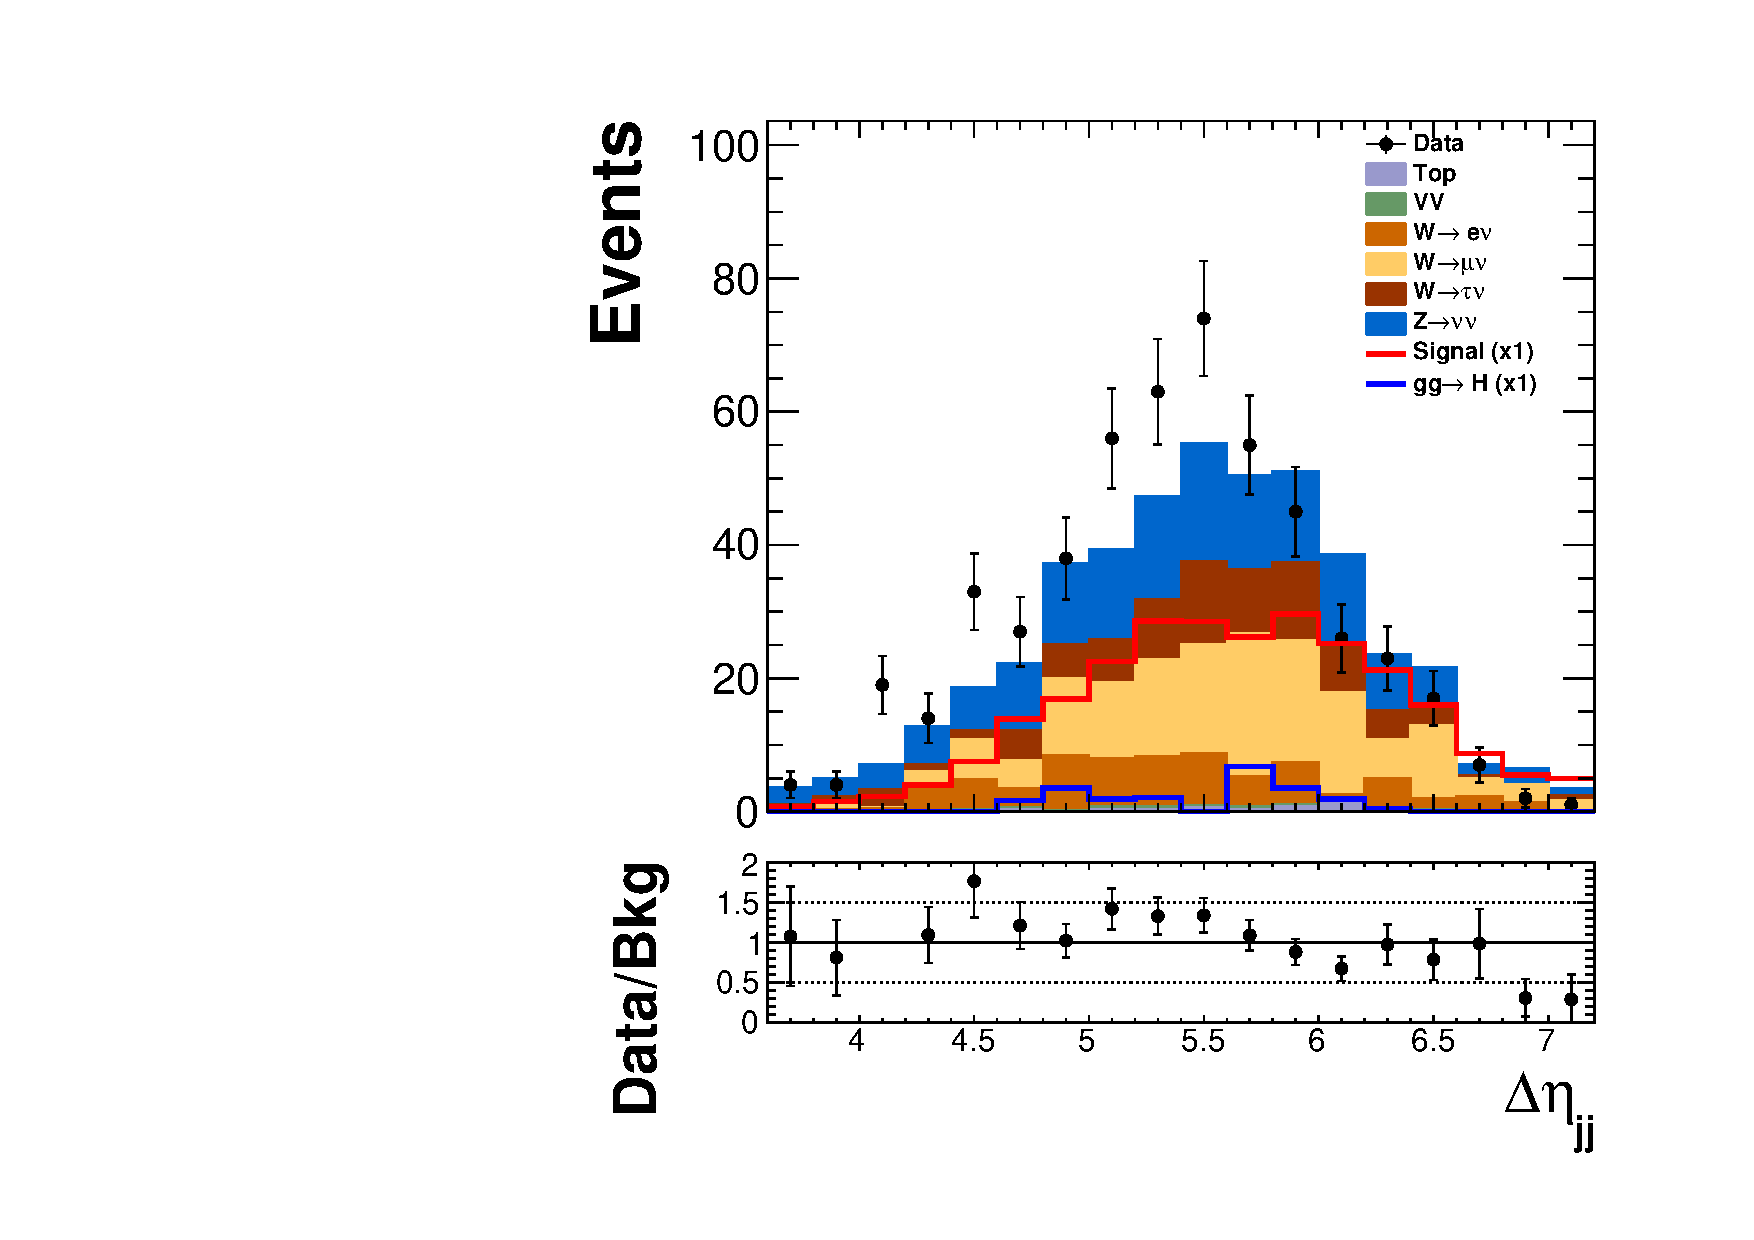
\includegraphics[width=.49\textwidth]{Chapter07/CrossCheck/Signal/sigRegion_Dijet_DeltaEta.pdf}}
\subfloat[]{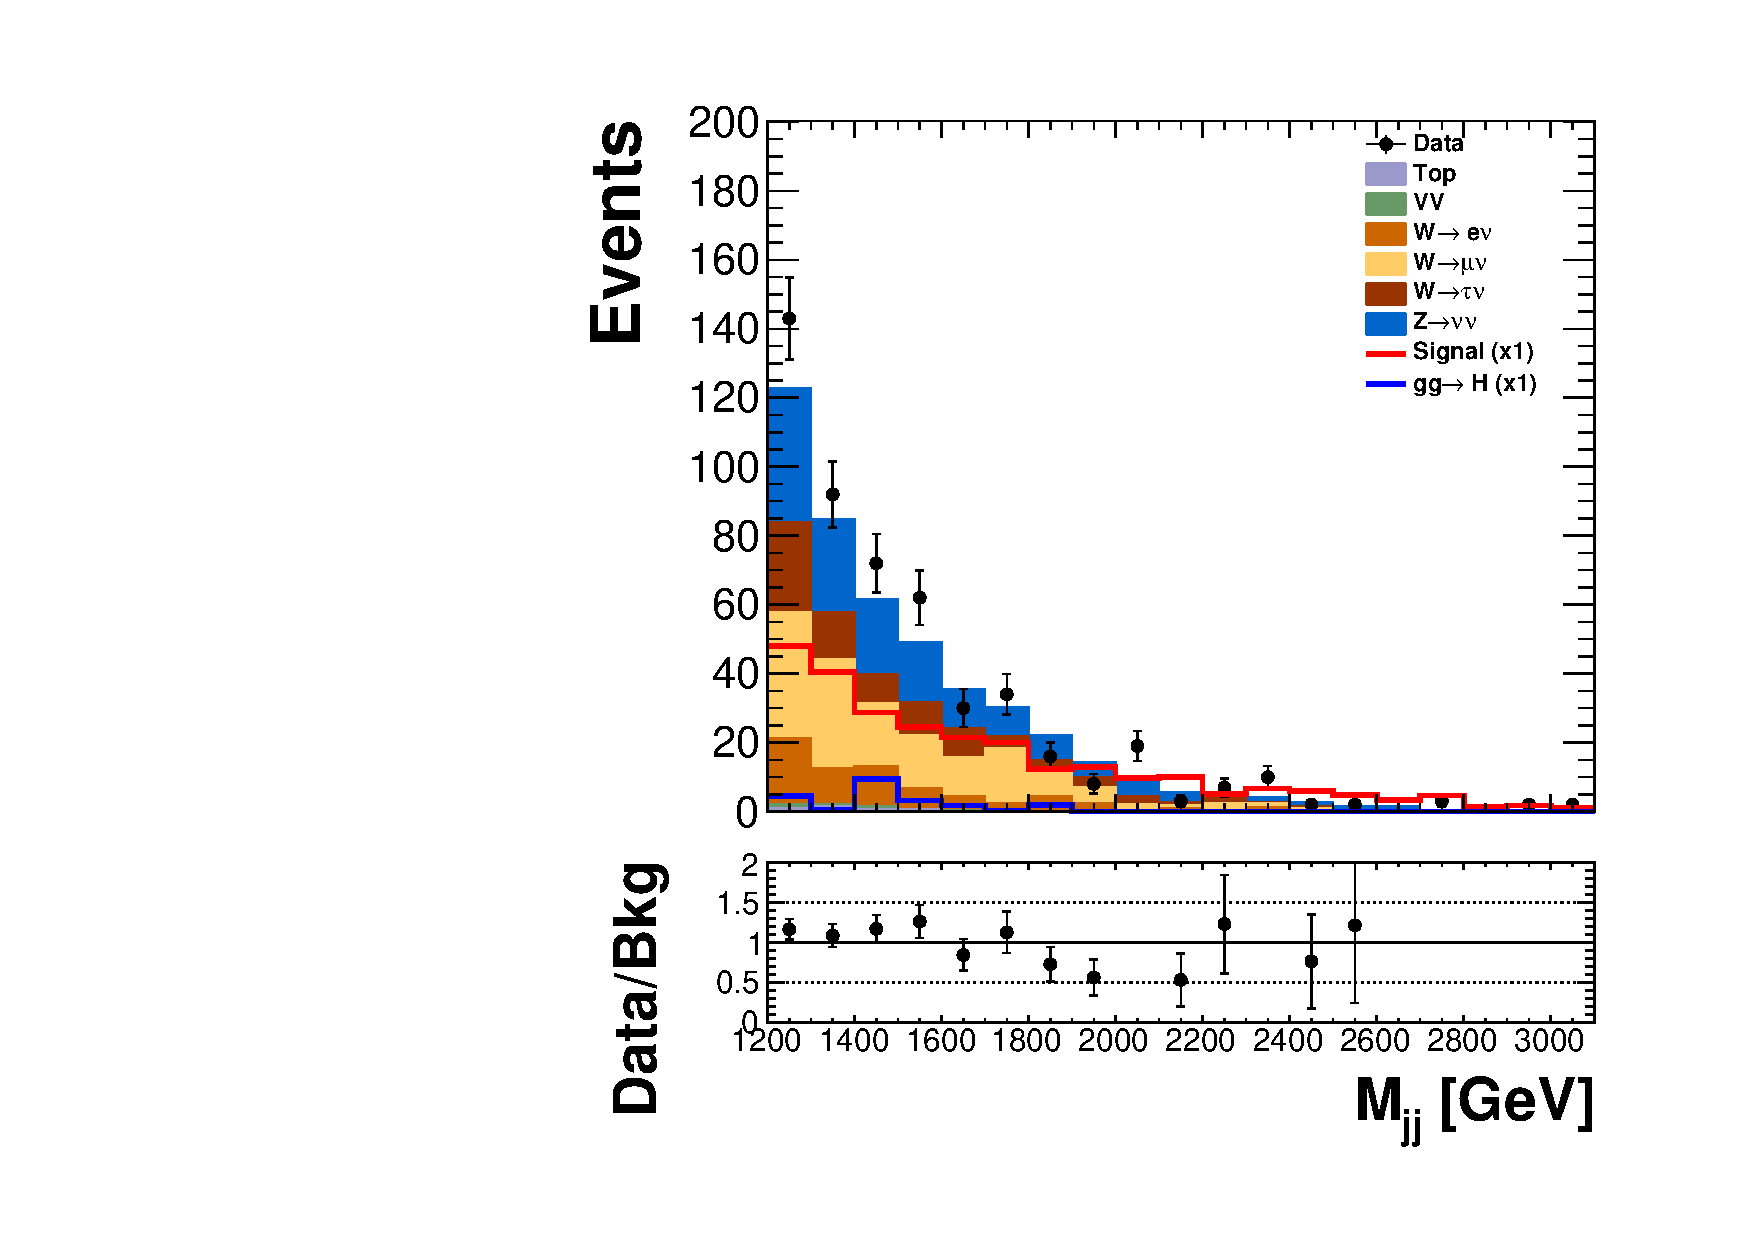
\includegraphics[width=.49\textwidth]{Chapter07/CrossCheck/Signal/sigRegion_Dijet_Mjj.pdf}} \\
\subfloat[]{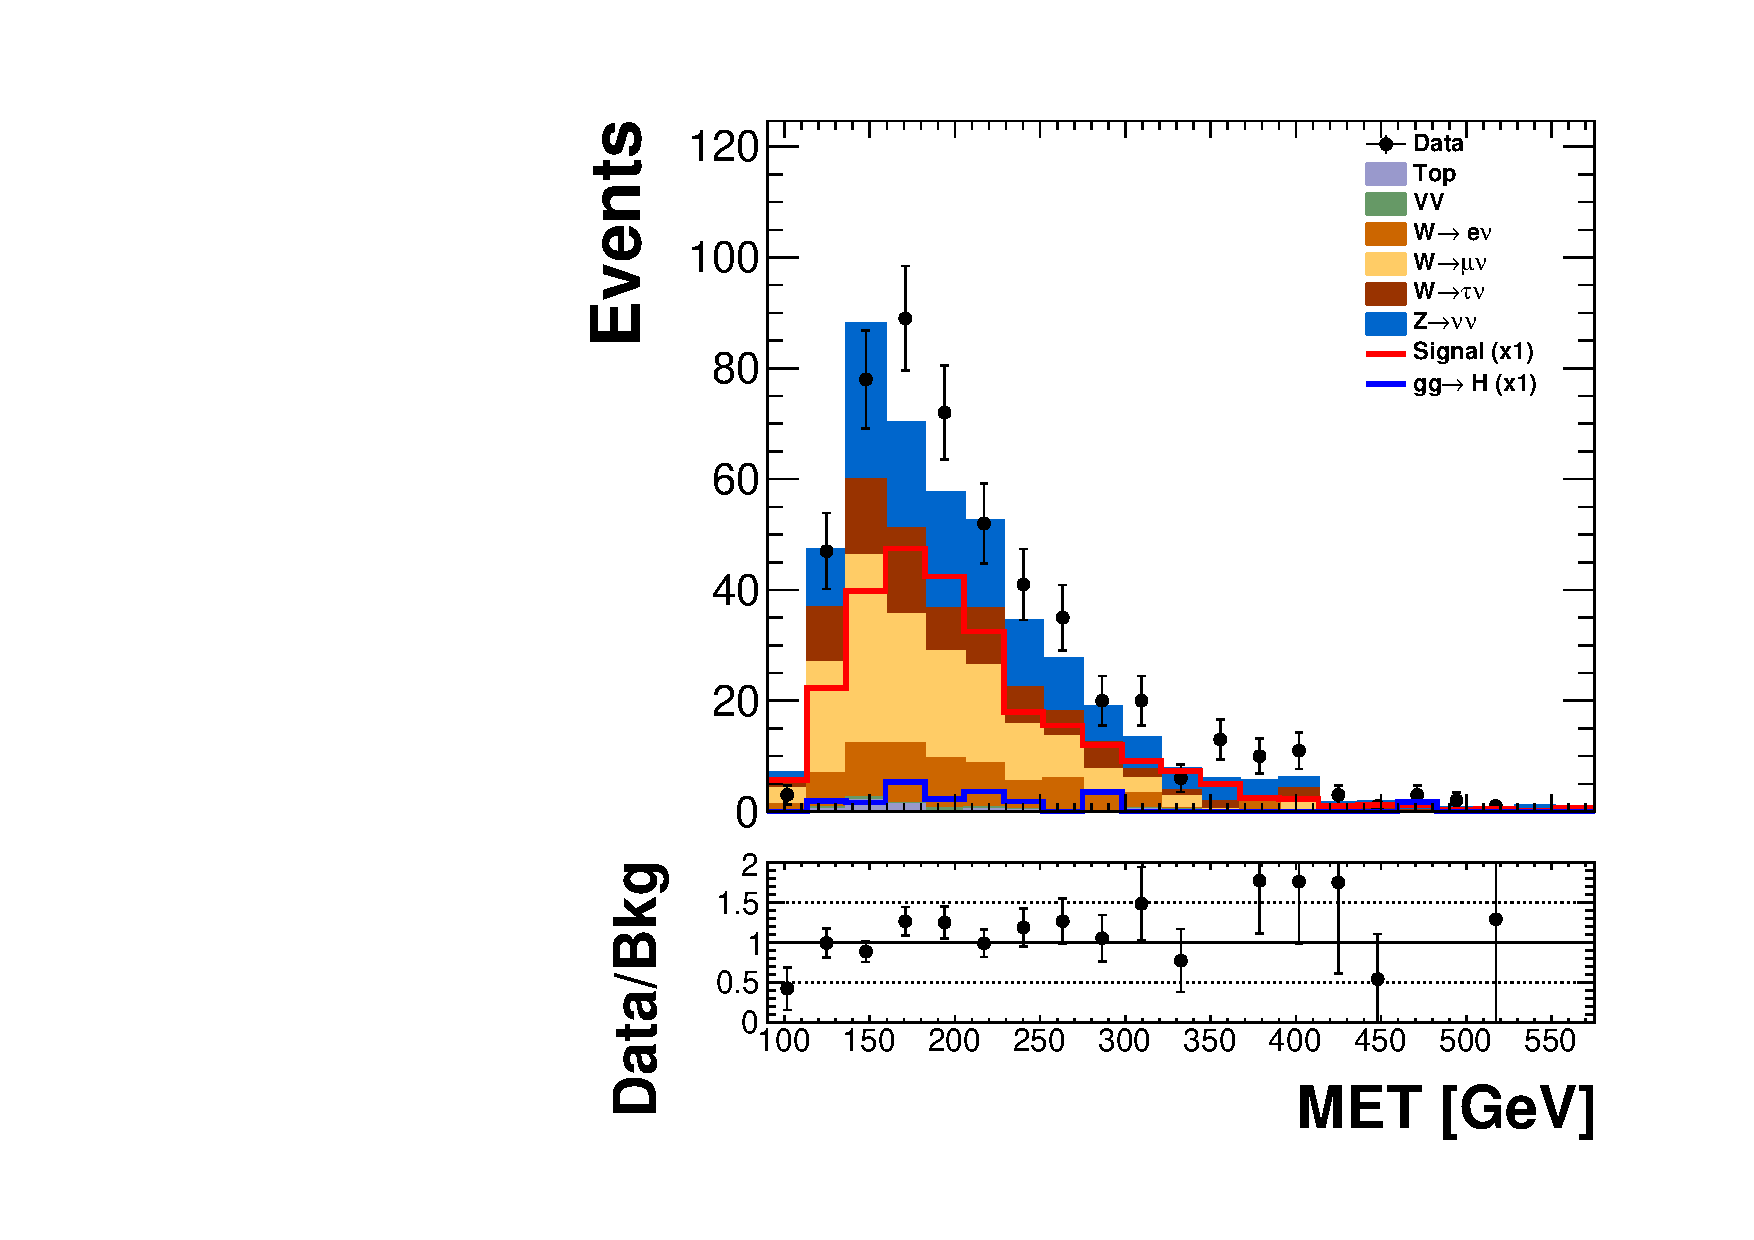
\includegraphics[width=.49\textwidth]{Chapter07/CrossCheck/Signal/sigRegion_metNoMuon.pdf}}
\subfloat[]{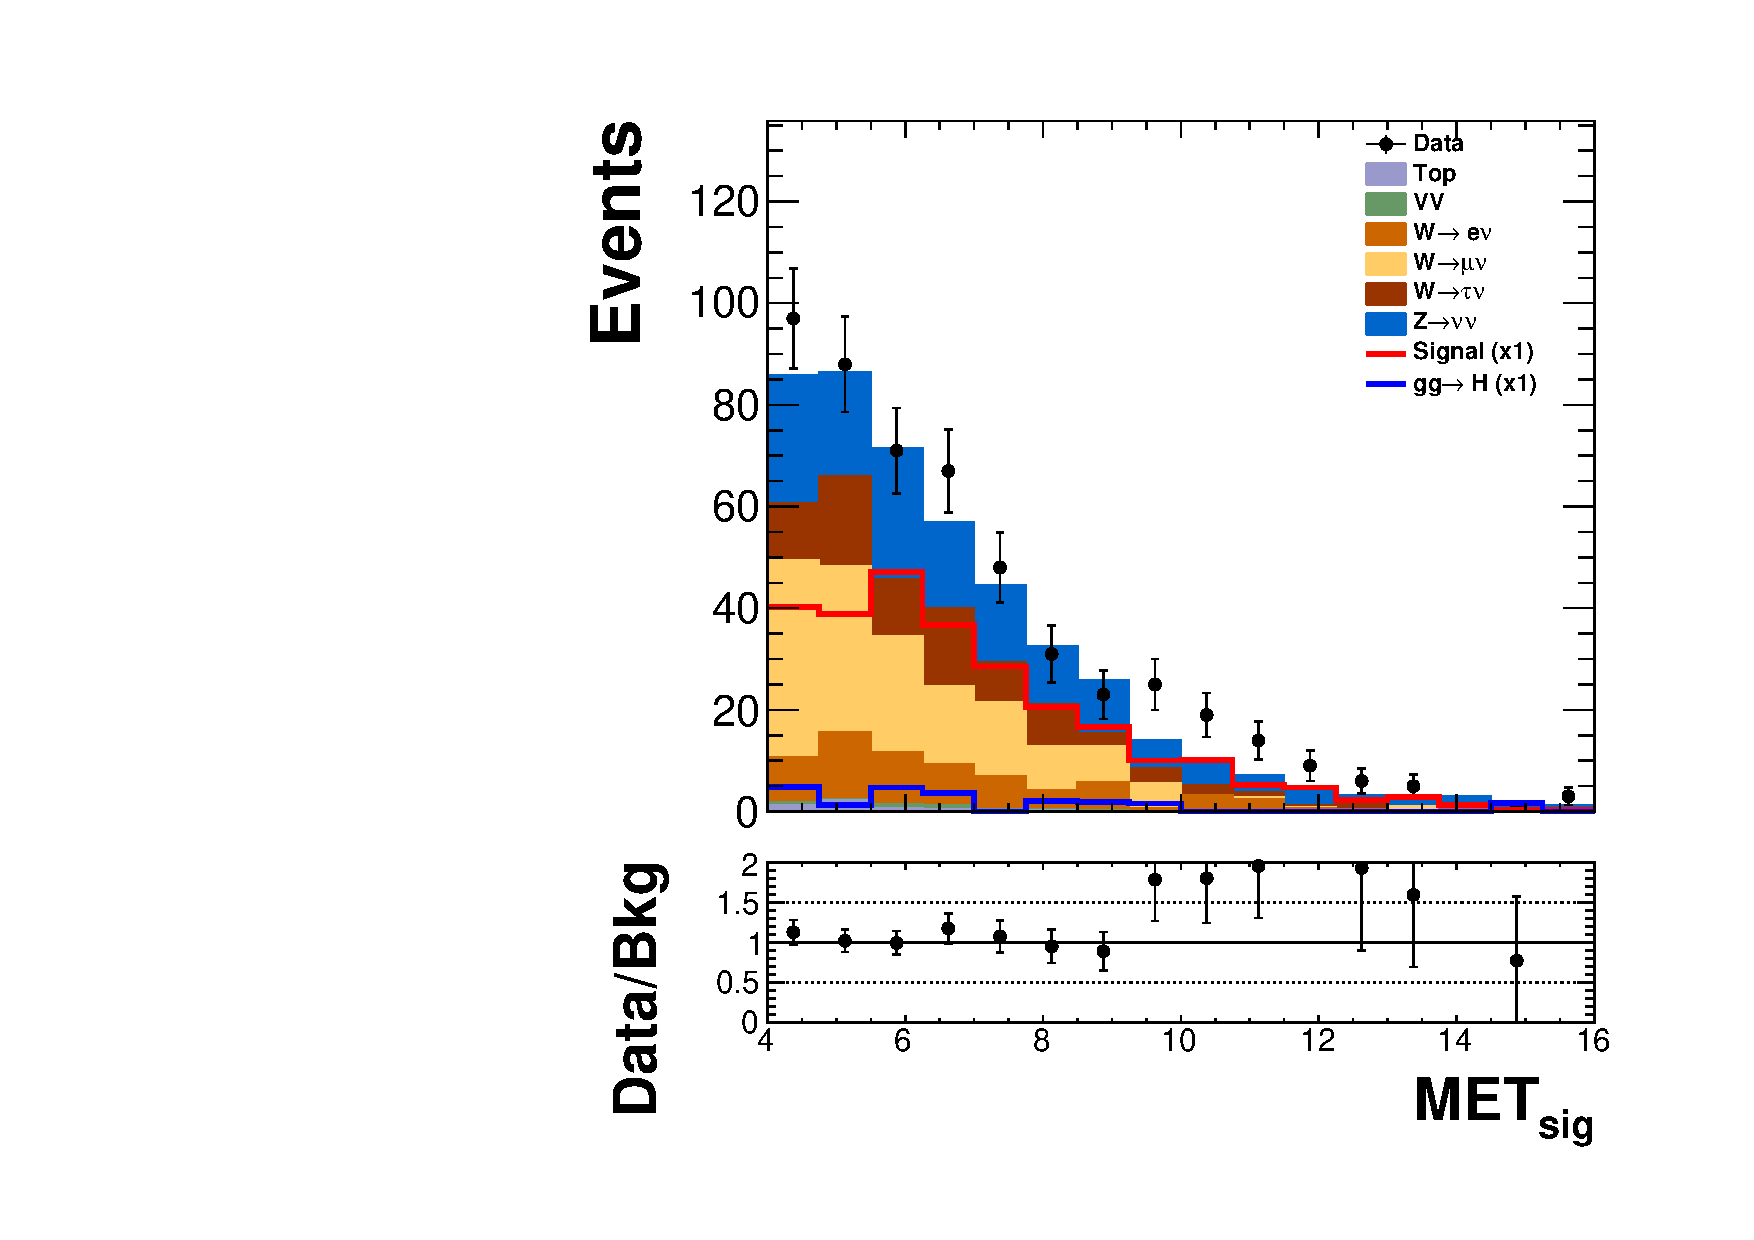
\includegraphics[width=.49\textwidth]{Chapter07/CrossCheck/Signal/sigRegion_metNoMuon_Sig.pdf}}
\caption[Pseudorapidity difference between the two selected VBF jets $\Delta\eta_{jj}$, dijet mass $M_{jj}$, MET significance $\text{MET}_{sig}$ and MET, in the signal region as produced by the cross check analysis.]
{(a) Pseudorapidity difference between the two selected \gls{VBF} jets $\Delta\eta_{jj}$, (b) dijet mass $M_{jj}$, (c) \gls{MET} significance $\text{MET}_{sig}$ and (d) \gls{MET}, in the signal region as produced by the cross check analysis.}
\label{FIGURE:ParkedDataAnalysis_Results_SigRegPlots}
\end{figure}

% Main
% \begin{figure}[!htb]
% \centering
% \subfloat[]{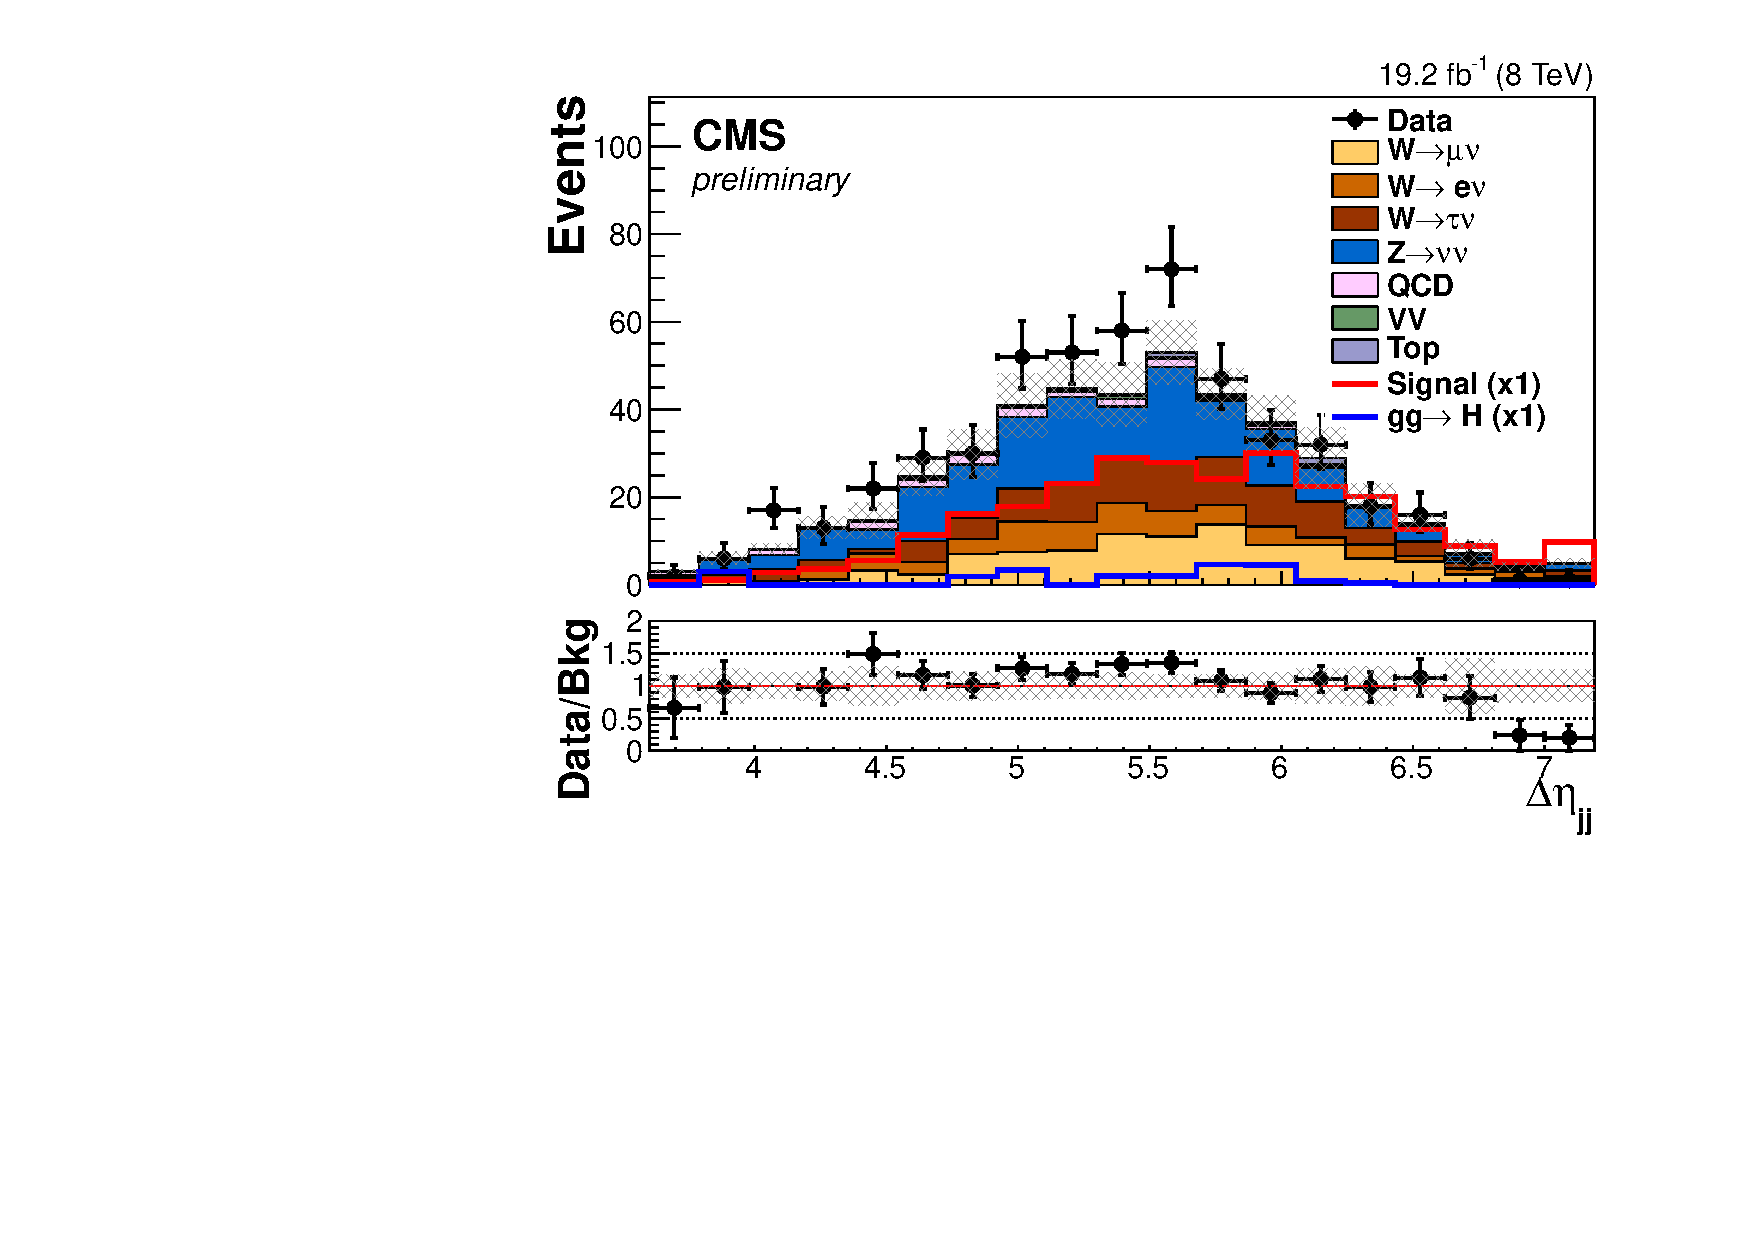
\includegraphics[width=.45\textwidth]{Chapter07/Images/output_sigreg/nunu_dijet_deta.pdf}}
% \subfloat[]{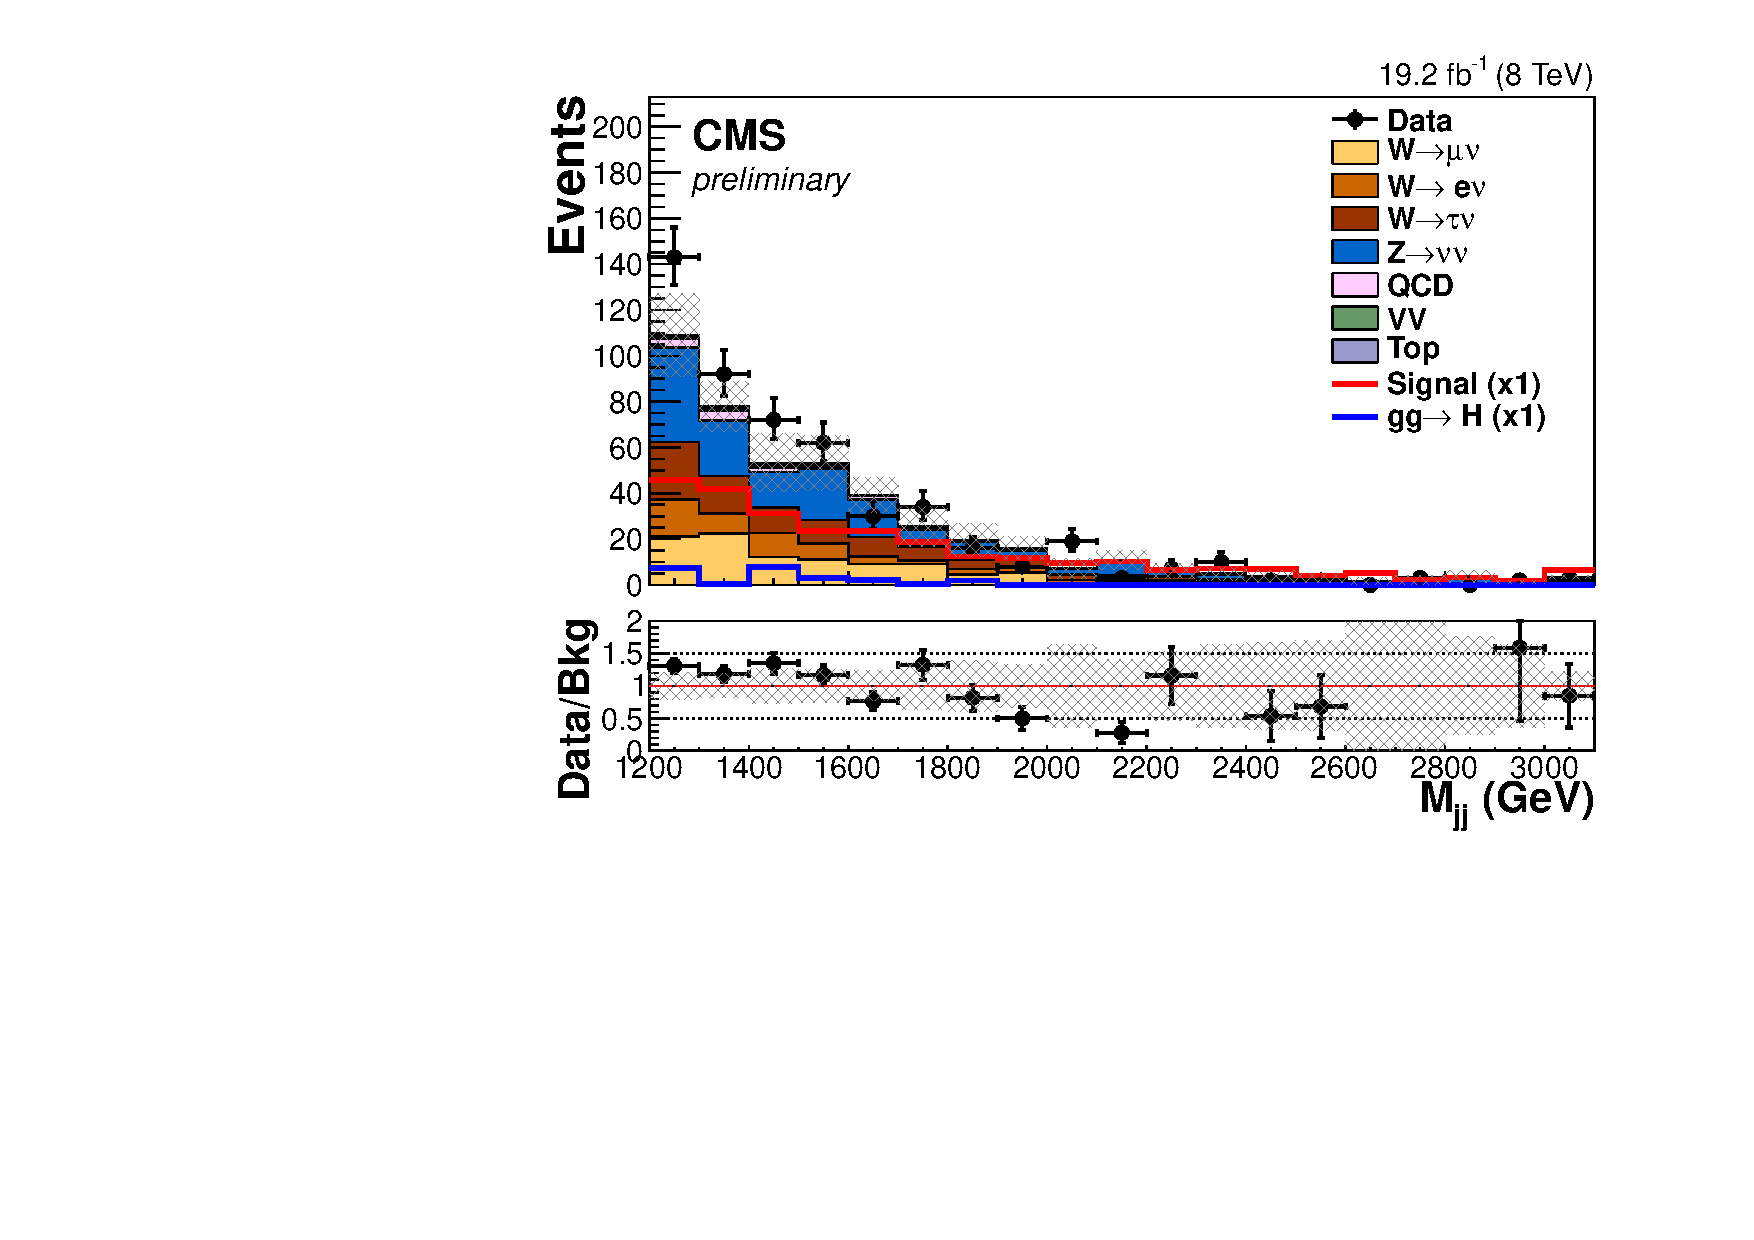
\includegraphics[width=.45\textwidth]{Chapter07/Images/output_sigreg/nunu_dijet_M.pdf}} \\
% \subfloat[]{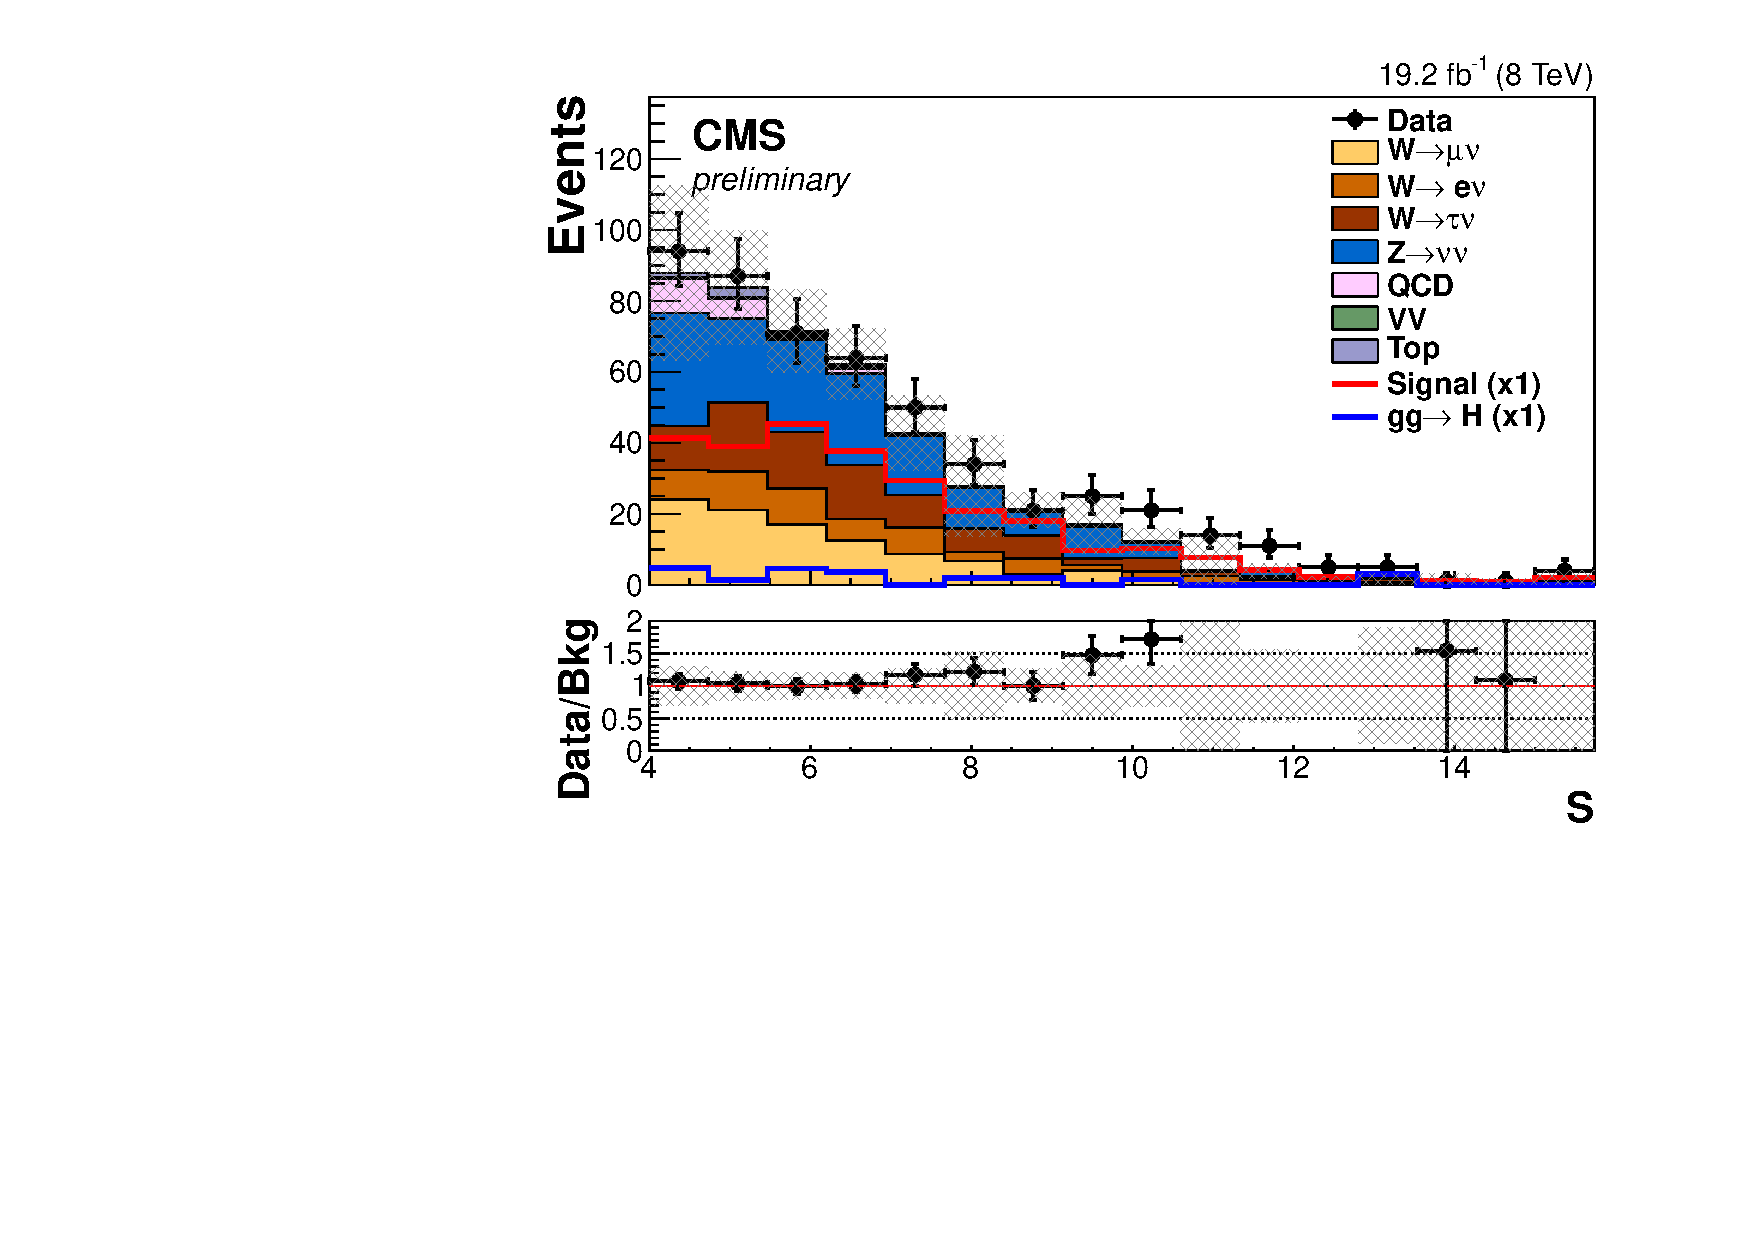
\includegraphics[width=.45\textwidth]{Chapter07/Images/output_sigreg/nunu_metnomu_significance.pdf}}
% \subfloat[]{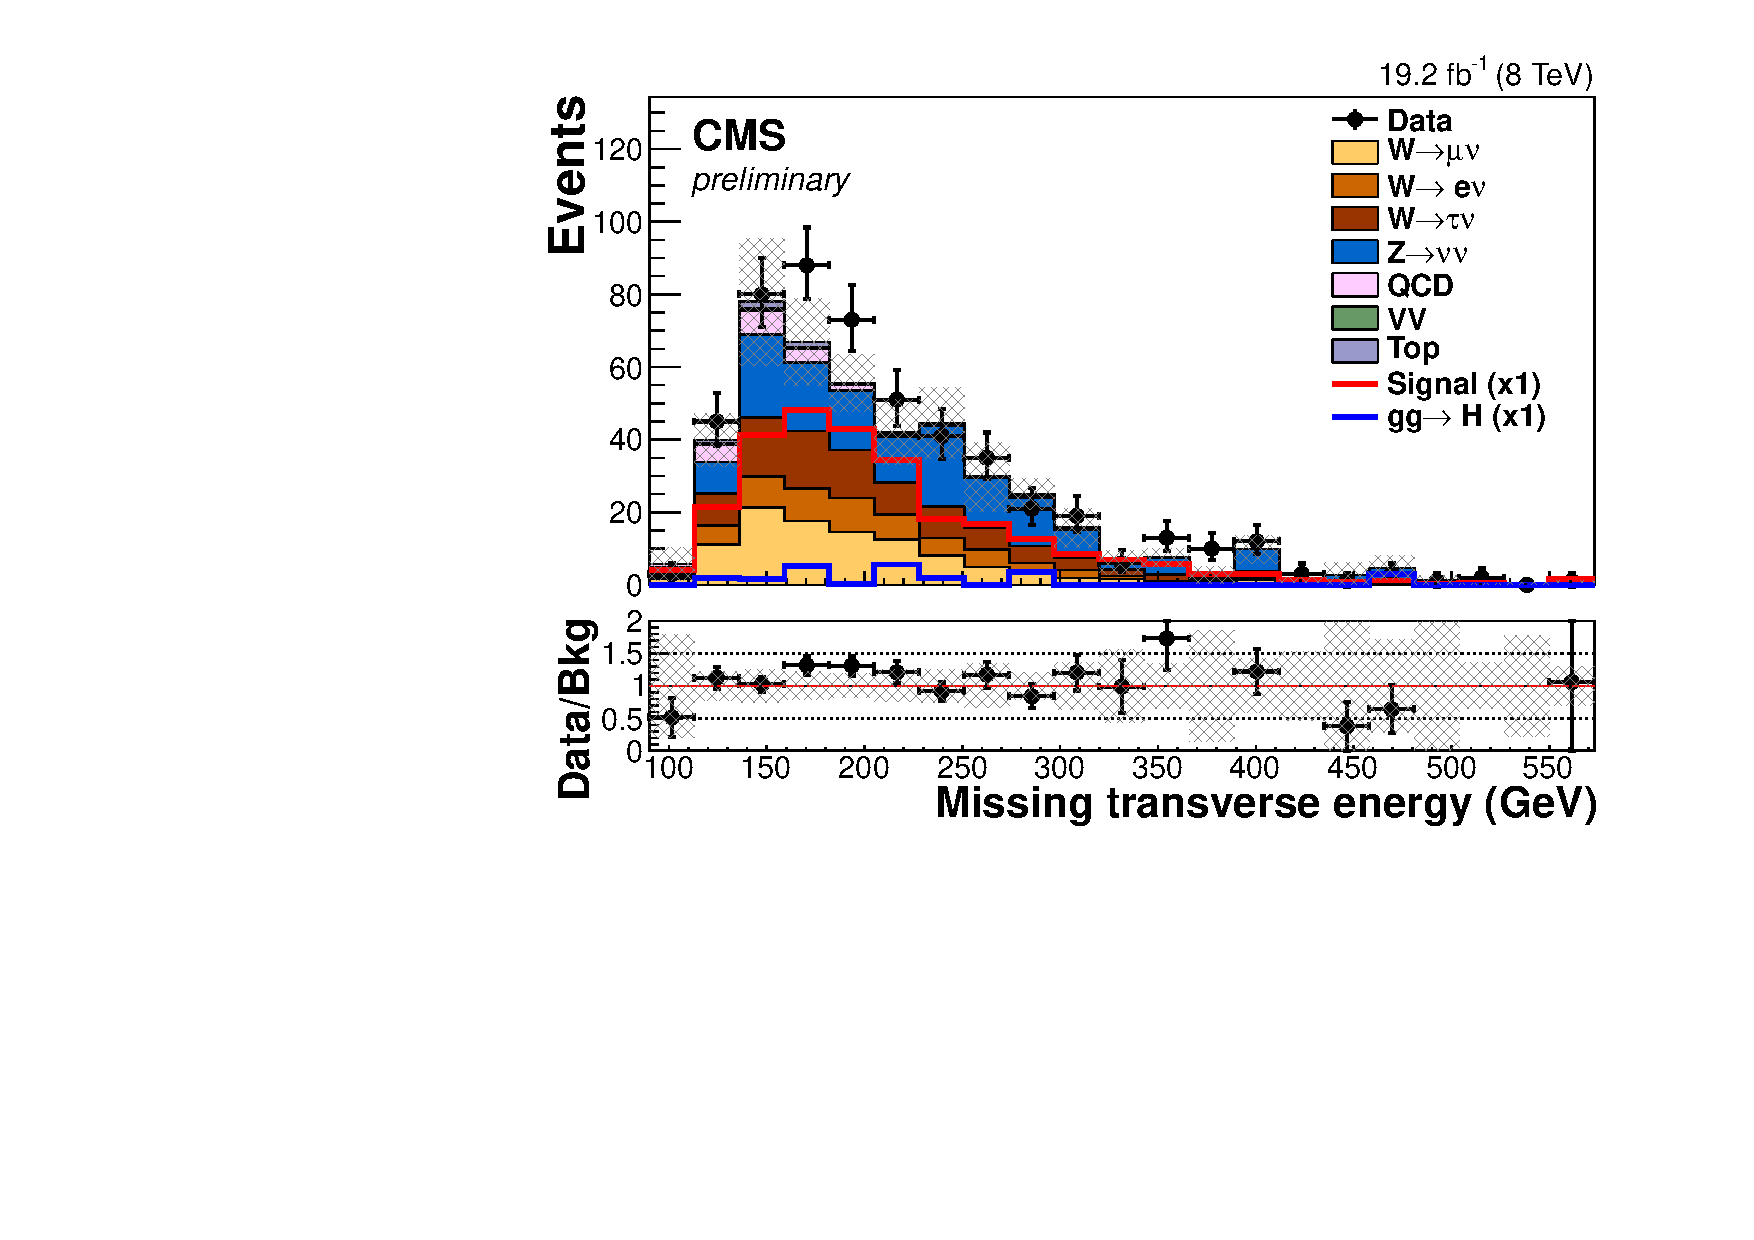
\includegraphics[width=.45\textwidth]{Chapter07/Images/output_sigreg/nunu_metnomuons.pdf}}
% \caption{(a) Pseudorapidity difference between the two selected \gls{VBF} jets $\Delta\eta_{jj}$, (b) dijet mass $M_{jj}$, (c) \gls{MET} significance $\text{MET}_{sig}$; and (d) \gls{MET}, in the signal region. The last bin represents all those events falling above the range of the histogram. An excess is seen which is less than 2$\sigma$ in significance as can be observed from the hatched band which indicates the size of the total uncertainty on the background estimate \cite{ARTICLE:CMSVBFHiggsInvisibleParkedAnalysisPAS}.}
% \label{FIGURE:ParkedDataAnalysis_Results_SigRegPlots}
% \end{figure}

\clearpage

%%%%%%%%%%%%%%%%%%%%%%%%%%%%%%%%%%%%%%%%%%%%%%%%%%%%%%%%%%%%%%%%%%%%%%%%%%%%%%%%%%%%
%%% SUBSECTION
%%%%%%%%%%%%%%%%%%%%%%%%%%%%%%%%%%%%%%%%%%%%%%%%%%%%%%%%%%%%%%%%%%%%%%%%%%%%%%%%%%%%
\subsection{Comparison with the cross-check analysis}

%Status: DONE (reviewed J.Pela x1)

The cross check analysis has successfully validated the main analysis by reproducing the data event yields in all the relevant regions. All event yields were measured to be exactly the same in both analysis except the yield in the \gls{QCD} sideband region where a discrepancy of +1.1\% was observed. Since the \gls{QCD} multi-jet background is a minor background, representing less than 4\% of the total background, this level of synchronization was deemed acceptable. Table \ref{TABLE:ParkedDataAnalysis_Results_MainCrossCheckComparison} shows a comparison of the event yield obtained by both analysis and the fractional difference for each region.

\begin{table}[!htb]
\centering
\begin{tabular}{|l|c|c|c|}
\hline
Region                & Main & Cross Check & Difference [\%] \\
\hline\hline
$Z\rightarrow\nu\nu$  &   18 &          18 &             0.0 \\
$W\rightarrow\mu\nu$  &  300 &         300 &             0.0 \\
$W\rightarrow e\nu$   &   68 &          68 &             0.0 \\
$W\rightarrow\tau\nu$ &   76 &          76 &             0.0 \\
top (Region 1)        &   21 &          21 &             0.0 \\
QCD Sideband region   & 1586 &        1603 &            +1.1 \\
% QCD Region II         &  411 &         412 &            +0.2 \\
% QCD Norm3             & 1517 &        1523 &            +0.4 \\
\hline\hline
Signal                &  508 &         508 &             0.0 \\
\hline
\end{tabular}
\caption[Comparison of the data event yields in all relevant regions, between the main and cross check analyses.]
{Comparison of the data event yields in all relevant regions, between the main and cross check analyses. The column ''Difference`` is defined a $(N_{\text{Cross Check}}-N_{\text{main}})/N_{\text{main}}$.}
\label{TABLE:ParkedDataAnalysis_Results_MainCrossCheckComparison}
\end{table}

%%%%%%%%%%%%%%%%%%%%%%%%%%%%%%%%%%%%%%%%%%%%%%%%%%%%%%%%%%%%%%%%%%%%%%%%%%%%%%%%%%%%
%%% SECTION
%%%%%%%%%%%%%%%%%%%%%%%%%%%%%%%%%%%%%%%%%%%%%%%%%%%%%%%%%%%%%%%%%%%%%%%%%%%%%%%%%%%%
\section{Limits on the cross section of invisibly decaying Higgs bosons}
\label{SECTION:ParkedDataAnalysis_Limits}

%Status: DONE (reviewed J.Pela x1)

As shown in table \ref{TABLE:ParkedDataAnalysis_Results_Summary}, 508 data events were observed in the signal region, this yield is compatible with the background-only prediction. Since no evidence of signal is observed, 95\% \gls{CL} upper limits on the Higgs boson production cross section times branching fraction are computed. The limits are calculated using the asymptotic $\mathrm{CL}_\mathrm{s}$ method \cite{ARTICLE:CLsTechnique,ARTICLE:CLCompForCombiningSearchesWithSmallStat,ARTICLE:HandbookofLHCHiggsCrossSectionsDifferentialDistributions} based on asymptotic formulae \cite{ARTICLE:AsymptoticCLS}, following the standard \gls{CMS} Higgs boson searches combination technique \cite{ARTICLE:CMS_HiggsDiscovery,ARTICLE:HiggsCombination}. Systematic uncertainties are incorporated as nuisance parameters and treated according to the frequentist paradigm \cite{ARTICLE:HiggsCombination} and all correlations between processes are taken into account.

If \gls{SM} production cross sections and acceptances are assumed, the observed (expected) 95\% C.L. limit on \BRinv\, of a \gls{SM} $125\,\GeV$ Higgs boson is 57\% (40\%). Figure \ref{FIGURE:ParkedDataAnalysis_Limits_VBFLimit} shows the the 95\% C.L. limit on \BRinv and 95\% C.L. limit on the cross section times \BRinv\,, both under the assumption of \gls{SM} Higgs boson acceptances, as a function of Higgs mass.

\begin{figure}[!htb]
\centering
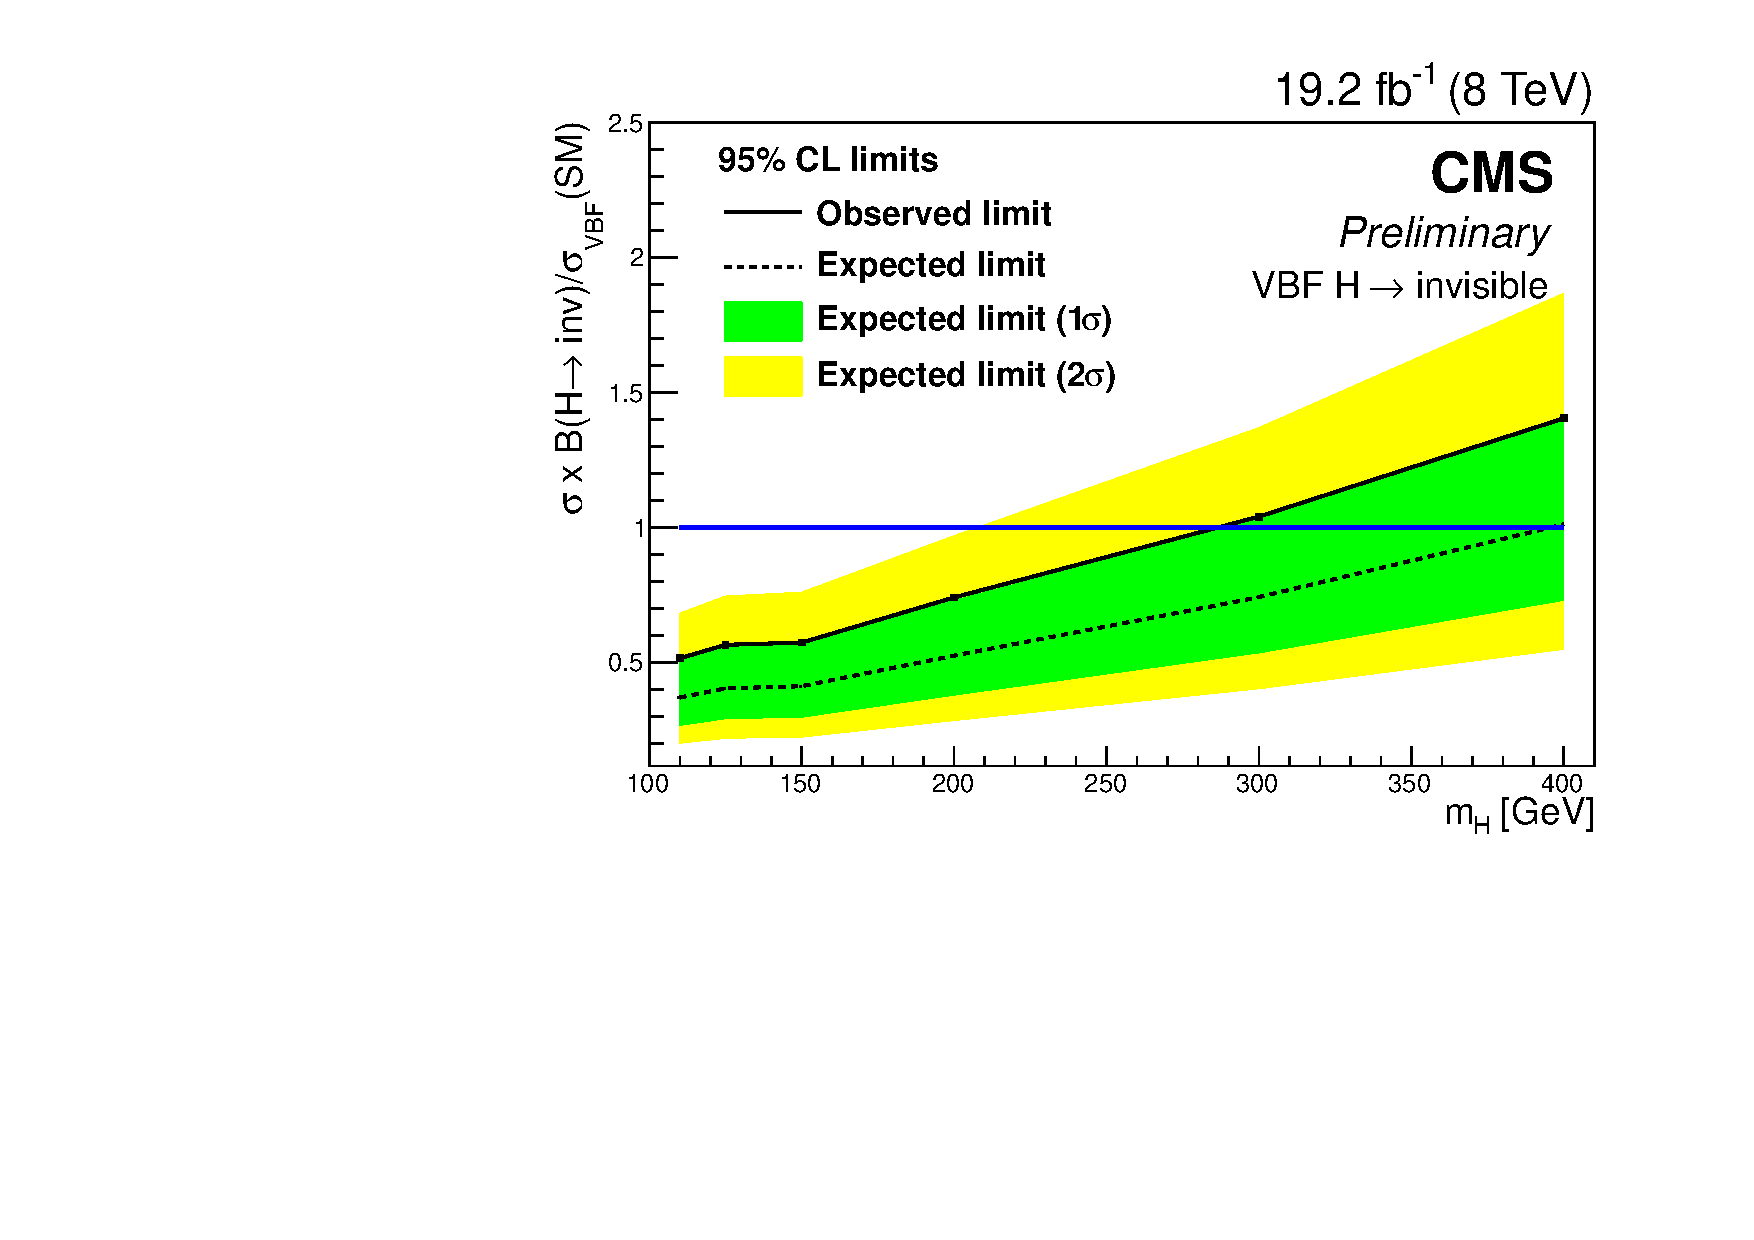
\includegraphics[width=0.49\textwidth]{Chapter07/Images/vbflimit.pdf}
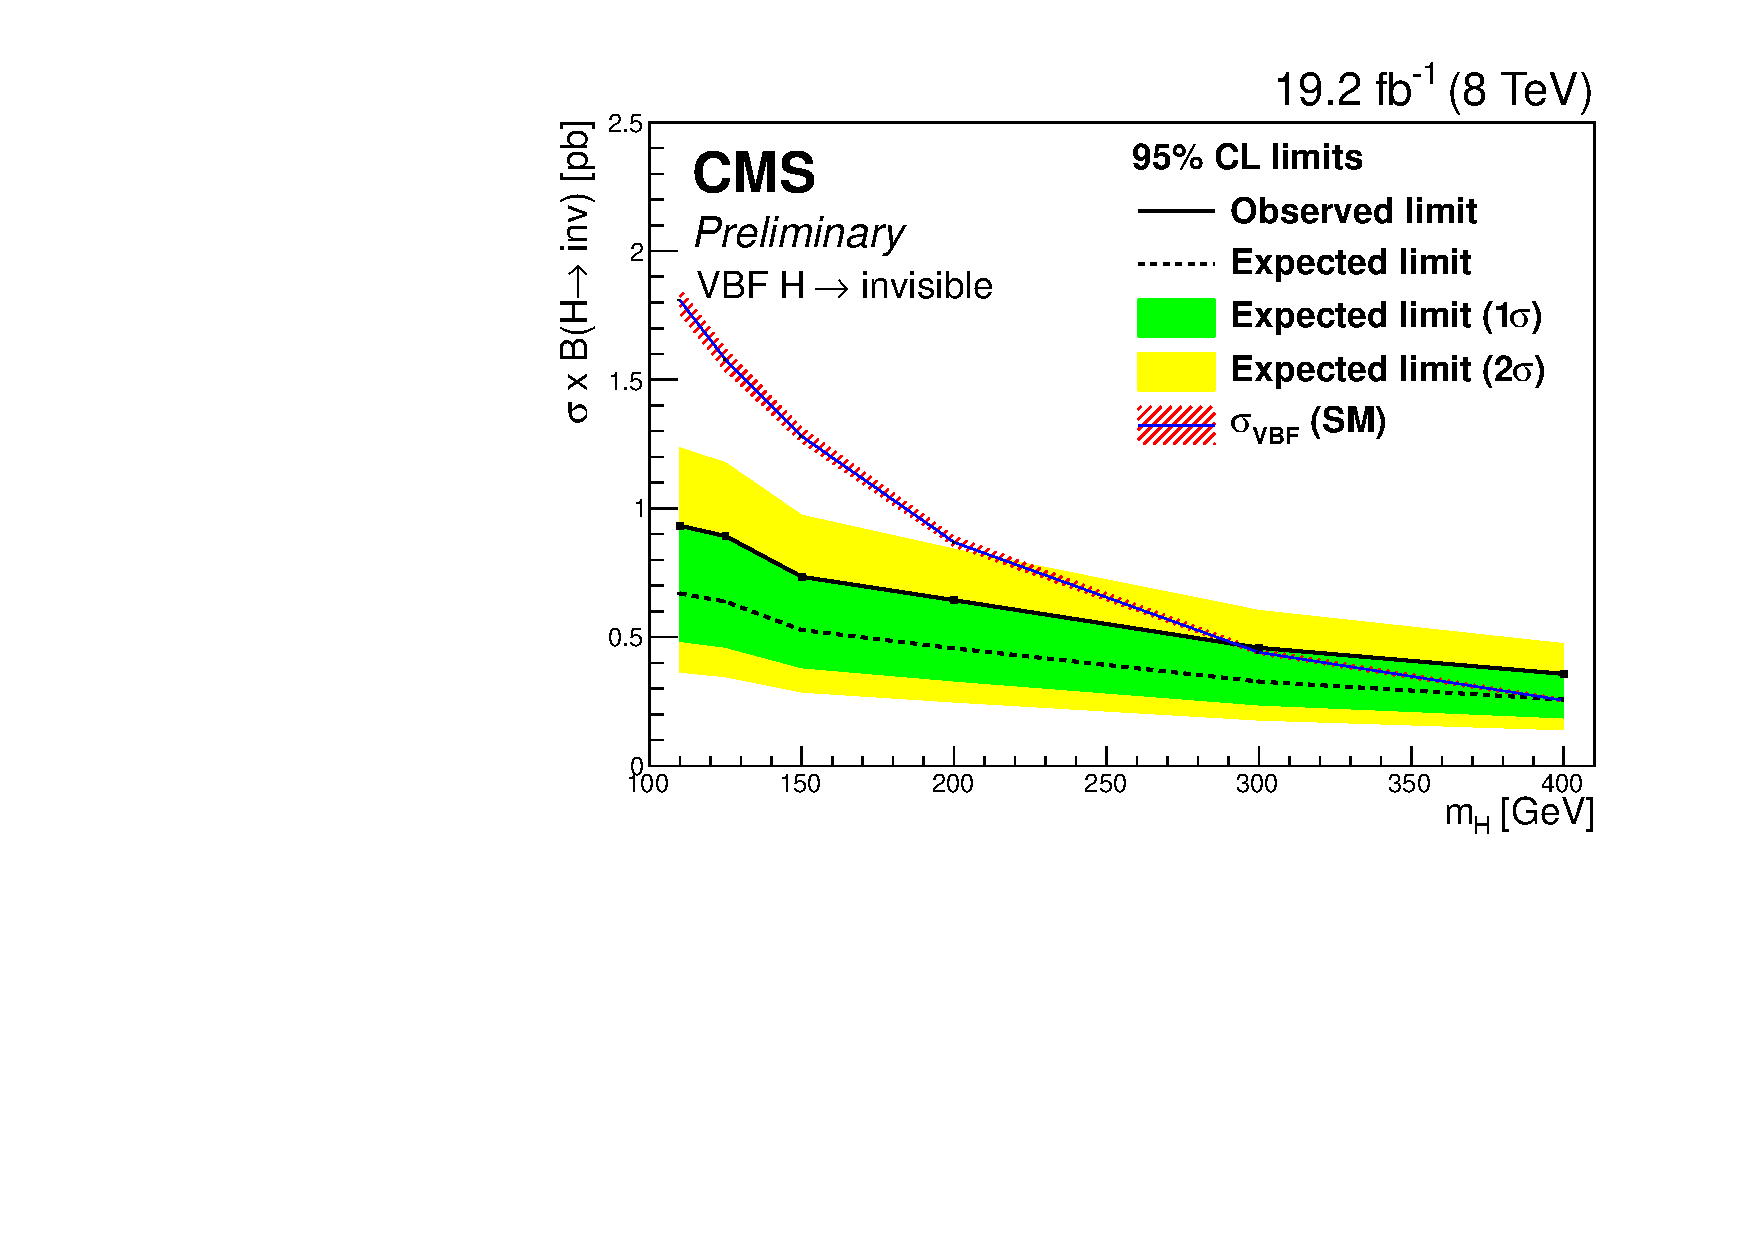
\includegraphics[width=0.49\textwidth]{Chapter07/Images/vbfxslimit.pdf}
\caption[The 95\% C.L. limit on \BRinv\, of a SM Higgs boson and the 95\% C.L. limit on the cross section times \BRinv\ as a function of the Higgs boson mass, assuming SM Higgs boson acceptances.]
{The 95\% C.L. limit on \BRinv\, of a SM Higgs boson (left) and the 95\% C.L. limit on the cross section times \BRinv\ (right) as a function of the Higgs boson mass, assuming SM Higgs boson acceptances~\cite{ARTICLE:CMSVBFHiggsInvisibleParkedAnalysisPAS}.}
\label{FIGURE:ParkedDataAnalysis_Limits_VBFLimit}
\end{figure}

As it can be observed in table \ref{TABLE:ParkedDataAnalysis_Systematics_Summary}, similarly to the \textit{prompt analysis}, the dominant source of systematic uncertainty is the limited number of events present in the control regions both in data and \gls{MC} simulation. This effect is particularly noticeable in the Z control region, if this region statistical uncertainty was of the order of the one measured in the $W\rightarrow\mu\nu$ control region the expected 95\% C.L. limit on the cross section times \BRinv for a \gls{SM} 125 GeV Higgs boson would be reduced to 33\%.

%TODO: Should I write the combined stuff???
% The result is also combined with that obtained by CMS in searches in the channel where the Higgs boson is produced in association with a Z which was reported in ~\cite{Chatrchyan:2014tja}. The procedure for this combination is also described in ~\cite{Chatrchyan:2014tja}. The 95\% C.L. observed (expected) limit on \BRinv\, after combination is 47\% (35\%) for a SM 125 GeV Higgs boson.
